\documentclass[conference]{IEEEtran}
% Compile with XeLaTeX (UTF-8 Vietnamese text).
\usepackage{fontspec}
\setmainfont{TeX Gyre Termes}
\usepackage{cite}
\usepackage{amsmath,amssymb,amsfonts}
\usepackage{algorithmic}
\usepackage{graphicx}
\usepackage{textcomp}
\usepackage{xcolor}
\usepackage{booktabs}
\usepackage{tabularx}
\usepackage{hyperref}

\begin{document}

\title{Phát Hiện Đặc Trưng Ảnh Đa Tỷ Lệ Bằng Đạo Hàm Gaussian: Cài Đặt Thuần NumPy và Thẩm Định Đối Chuẩn với FeatureJ / Fiji}

\author{\IEEEauthorblockN{Nguyễn Đức Mạnh, Bùi Trung Đức, Phạm Bảo Lộc, Nguyễn Tiến Hưng}
\IEEEauthorblockA{\textit{Khoa Công nghệ Thông tin - Môn Xử lý ảnh số (XLA)}}
}

\maketitle

\begin{abstract}
Báo cáo trình bày cơ sở toán học, cài đặt NumPy và đánh giá hệ thống phát hiện đặc trưng ảnh đa tỷ lệ dựa trên đạo hàm Gaussian; FeatureJ/Fiji được dùng làm tham chiếu cho các bản đồ vi phân. Tầng 1 đối chiếu 220 bản đồ liên tục trên 5 ảnh: 35 bản đồ đạt đồng thời ngưỡng gốc $\mathrm{rel\_err}<10^{-4}$ và Pearson $r>0.9999$, còn 185 bản đồ đạt tiêu chí nới lỏng đã định trước. Tầng 2 đánh giá trên 25 ảnh BSDS500, DRIVE và Blobs; snapshot canonical tại commit \texttt{58bdfd8} cho F1 Python/Fiji ở BSDS $\sigma=2$ là 0.477886/0.477886, DRIVE macro là 0.680633/0.681651 và Blob macro là 0.893023/0.891901. Blob micro F1 là 0.492114/0.486656. Benchmark 36 trường hợp, 5 lần lặp, ghi nhận tốc độ chập tách rời cao hơn 1.375738--31.392971 lần và sai khác tuyệt đối tối đa $1.279\times10^{-12}$. Giao thức BSDS dùng dung sai đĩa Euclidean bán kính 2 pixel; ngưỡng được chọn trên tập ảnh thực nghiệm nên kết quả không được diễn giải như điểm kiểm tra độc lập.
\end{abstract}

\begin{IEEEkeywords}
Scale-space, Gaussian Derivatives, FeatureJ, Edge Detection, Ridge Detection, Blob Detection, Frangi Vesselness, Structure Tensor.
\end{IEEEkeywords}

\section{Chương 1: Giới Thiệu Chung}

\subsection{Bối Cảnh và Thách Thức của Xử Lý Ảnh Đa Tỷ Lệ}
Trong thị giác máy tính và xử lý ảnh y sinh hiện đại, các đối tượng hình thái học như đường biên (edges), mạng lưới mạch máu hình ống (ridges/vessels) và các cụm tế bào (blobs) xuất hiện ở vô số kích thước vật lý khác nhau tùy thuộc vào khoảng cách chụp, độ phân giải cảm biến và bản chất giải phẫu học. Một trong những nghịch lý cơ bản của xử lý ảnh là: \textit{không tồn tại một kích thước cửa sổ lọc cố định nào có thể đồng thời làm nổi bật mọi chi tiết từ nhỏ li ti đến các cấu trúc bao quát toàn cục}.

Nếu dùng bộ lọc cục bộ quá nhỏ, nhiễu tần số cao có thể ảnh hưởng rõ đến đáp ứng. Một cửa sổ quá lớn lại làm nhòe ranh giới và giảm các chi tiết nhỏ. Vì thế cần khảo sát đáp ứng ở nhiều tỷ lệ thay vì dựa vào một kích thước lọc cố định.

\subsection{Hạn Chế của Các Toán Tử Rời Rạc Cổ Điển}
Trong các giáo trình xử lý ảnh truyền thống, các bộ vi phân hữu hạn như Sobel, Prewitt, Roberts hay toán tử Laplace rời rạc $3 \times 3$ thường được sử dụng do chi phí tính toán thấp. Tuy nhiên, các toán tử này có một số hạn chế khi cần phân tích đa tỷ lệ:
\begin{enumerate}
    \item \textbf{Tính bất đẳng hướng và nhạy cảm với hướng trục:} Các mặt nạ $3 \times 3$ xấp xỉ đạo hàm theo sai phân hữu hạn làm biến dạng đáp ứng theo các góc chéo ($45^\circ, 135^\circ$), làm sai lệch góc hướng gradient $\theta = \arctan(L_y / L_x)$.
    \item \textbf{Thiếu vắng tham số tỷ lệ thực sự:} Các toán tử vi phân rời rạc không có cơ chế điều chỉnh độ rộng dải thông một cách liên tục và chặt chẽ về mặt vật lý.
    \item \textbf{Khuếch đại nhiễu bậc cao:} Phép vi phân bản chất là bộ lọc thông cao, do đó việc tính đạo hàm bậc 2 trực tiếp trên ảnh số rời rạc mà không có bộ lọc Gaussian tiền trạm sẽ làm bùng nổ phương sai của nhiễu nền, có thể làm các đáp ứng Hessian nhiễu và kém ổn định.
\end{enumerate}

\subsection{Cơ Sở Thiết Kế và Động Lực Nghiên Cứu}
Lý thuyết không gian tỷ lệ tuyến tính (Linear Scale-Space Theory) cung cấp khuôn khổ để khảo sát ảnh ở các độ mịn khác nhau. Dưới các giả thiết chuẩn về tính tuyến tính, bất biến tịnh tiến và tính nhất quán theo tỷ lệ, họ Gaussian có tính chất không tăng cường cực trị cục bộ theo diễn giải khuếch tán khi tăng mức làm mịn \cite{witkin1983scale,lindeberg1994scale}.

Trong nghiên cứu này, FeatureJ (ImageScience trong Fiji/ImageJ) được chọn làm bộ cài đặt tham chiếu để đối chiếu các bản đồ đạo hàm. Nhân Python được viết từ các công thức toán học bằng NumPy; các phép đo tập trung vào mức độ tương đồng, sai số còn lại và ảnh hưởng của cách rời rạc hóa. Phạm vi đối chiếu này không xem FeatureJ là nhãn chân lý cho chất lượng phát hiện, vì hai câu hỏi đó được đánh giá riêng bằng Ground Truth ở Tầng 2.

\subsection{Mục Tiêu và Nội Dung Kỹ Thuật của Đề Tài}
Báo cáo tập trung vào bốn nội dung kỹ thuật:
\begin{itemize}
    \item \textbf{Nhân toán học NumPy:} Trong \texttt{src/core/}, tự cài đặt tích chập tách trục, đạo hàm Gaussian bậc 0--2, chuẩn hóa tỷ lệ, trị riêng Hessian và ten-xơ cấu trúc; phần lõi không thay các phép toán này bằng bộ lọc OpenCV hoặc SciPy.
    \item \textbf{Đối chiếu tham số rời rạc hóa của FeatureJ:} Khảo sát bán kính kernel, cách xử lý biên, chuẩn hóa tỷ lệ và thứ tự trị riêng bằng cấu hình plugin và phép đo trên các ảnh hiệu chuẩn.
    \item \textbf{Bảo toàn moment rời rạc Taylor:} Cài đặt kernel bậc 0, 1, 2 với các ràng buộc moment phù hợp, sau đó đo sai số còn lại khi so với FeatureJ thay vì giả định hai bộ cài đặt phải trùng tuyệt đối.
    \item \textbf{Khung đánh giá hai tầng:} Tầng 1 đối chiếu 220 bản đồ với FeatureJ trên 5 ảnh; Tầng 2 đánh giá trên 25 ảnh BSDS500, DRIVE và Blobs bằng nhãn tham chiếu (trong đó bốn ảnh Blobs là ảnh tổng hợp).
\end{itemize}

\subsection{Bố Cục của Báo Cáo Kỹ Thuật}
Nội dung báo cáo được cấu trúc thành 6 chương:
\begin{itemize}
    \item \textbf{Chương 1:} Giới thiệu tổng quan, đặt vấn đề và mục tiêu đề tài.
    \item \textbf{Chương 2:} Cơ sở lý thuyết không gian tỷ lệ Gaussian, đạo hàm vi phân chuẩn hóa, ma trận Hessian và các thuật toán phát hiện đặc trưng mức cao.
    \item \textbf{Chương 3:} Khảo sát FeatureJ, quy trình xuất bản đồ và tự động hóa bằng Fiji Macro / Java exporter.
    \item \textbf{Chương 4:} Thiết kế kiến trúc và giải pháp cài đặt hệ thống lõi Python thuần NumPy from scratch.
    \item \textbf{Chương 5:} Thực nghiệm định lượng, phân tích sai số đối chuẩn Tầng 1 và đánh giá Tầng 2 trên nhãn tham chiếu.
    \item \textbf{Chương 6:} Kết luận, đánh giá mức độ hoàn thành và định hướng mở rộng hệ thống.
\end{itemize}

\section{Chương 2: Cơ Sở Lý Thuyết và Ý Nghĩa Các Đặc Trưng}
\subsection{Mô hình ảnh và quy ước tọa độ}
Ảnh xám được mô tả bởi hàm cường độ $I(x,y)$; trên máy tính, ảnh là ma trận $I[j,i]$ với cột $i$ tương ứng trục $x$ và hàng $j$ tương ứng trục $y$. Trong dự án, $x$ tăng sang phải và $y$ tăng xuống dưới. Quy ước này cần được giữ giữa Python và Fiji: đổi hàng với cột sẽ hoán đổi $L_x,L_y$; đổi hướng trục có thể đổi dấu đạo hàm bậc lẻ dù hình dạng đáp ứng vẫn giống nhau.

Với ảnh màu, phép phân tích được thực hiện trên ảnh xám đã chuẩn hóa của bộ dữ liệu. Đặc biệt, ảnh DRIVE dùng trong repo đã được chuẩn bị cho bài toán mạch máu; không áp dụng thêm một phép chuyển đổi màu tùy ý cho riêng một nhánh. Cả hai bộ cài đặt phải đọc cùng dữ liệu đầu vào, cùng kích thước và cùng miền cường độ.

\subsection{Gaussian smoothing: công thức và vai trò}
Hạt nhân Gaussian hai chiều đẳng hướng có dạng
\begin{equation}
G_\sigma(x,y)=\frac{1}{2\pi\sigma^2}
\exp\left(-\frac{x^2+y^2}{2\sigma^2}\right),\qquad \sigma>0.
\label{eq:gaussian2d}
\end{equation}
Ảnh làm mịn được xác định bởi
\begin{equation}
L(x,y;\sigma)=(G_\sigma*I)(x,y).
\label{eq:scalespace}
\end{equation}
Mỗi pixel đầu ra là trung bình có trọng số của vùng lân cận; điểm gần tâm có trọng số lớn hơn điểm xa tâm. Vì $\int G_\sigma\,dx\,dy=1$, lọc Gaussian bảo toàn một ảnh hằng trong mô hình liên tục. Khi rời rạc hóa, tổng các hệ số kernel cần được chuẩn hóa về 1 để giữ tính chất tương ứng.

Tham số $\sigma$ là độ lệch chuẩn, đo bằng pixel nếu ảnh chưa hiệu chuẩn kích thước vật lý. $\sigma$ càng lớn, vùng lấy trung bình càng rộng: nhiễu và các biến thiên nhỏ giảm đi, nhưng ranh giới và chi tiết mảnh cũng có thể mờ hơn. Vì vậy làm mịn là một sự đánh đổi giữa ổn định trước nhiễu và bảo toàn độ phân giải không gian.

\subsubsection{Tính khả tách và chi phí tính toán}
Đặt $g_\sigma(x)=\exp(-x^2/2\sigma^2)/(\sqrt{2\pi}\sigma)$, ta có $G_\sigma(x,y)=g_\sigma(x)g_\sigma(y)$. Từ tính kết hợp của tích chập,
\begin{equation}
I*G_\sigma=(I*g_\sigma^{\,x})*g_\sigma^{\,y}.
\end{equation}
Thay một phép lọc $K\times K$ bằng hai phép lọc dài $K$ làm chi phí trên ảnh $H\times W$ giảm từ $\mathcal O(HWK^2)$ xuống $\mathcal O(HWK)$, với khoảng $2K$ phép nhân cộng cho mỗi pixel. Đây là tối ưu cấu trúc của Gaussian, không phải một xấp xỉ làm thay đổi mô hình toán học; sai khác thực tế vẫn có thể xuất hiện do cắt kernel và làm tròn.

\subsubsection{Giải thích trong miền tần số}
Với tần số tính bằng chu kỳ trên pixel, biến đổi Fourier của Gaussian là
\begin{equation}
\widehat G_\sigma(f_x,f_y)
=\exp[-2\pi^2\sigma^2(f_x^2+f_y^2)].
\end{equation}
Các thành phần tần số cao bị suy giảm mạnh hơn thành phần thấp. Phép đạo hàm theo $x$ lại nhân phổ với $2\pi \mathrm{i}f_x$, làm tăng ảnh hưởng của biến thiên nhanh. Kết hợp Gaussian và đạo hàm giúp đo sự thay đổi của ảnh ở một dải tỷ lệ xác định, đồng thời hạn chế sự khuếch đại nhiễu.


\begin{figure*}[t]
\centering
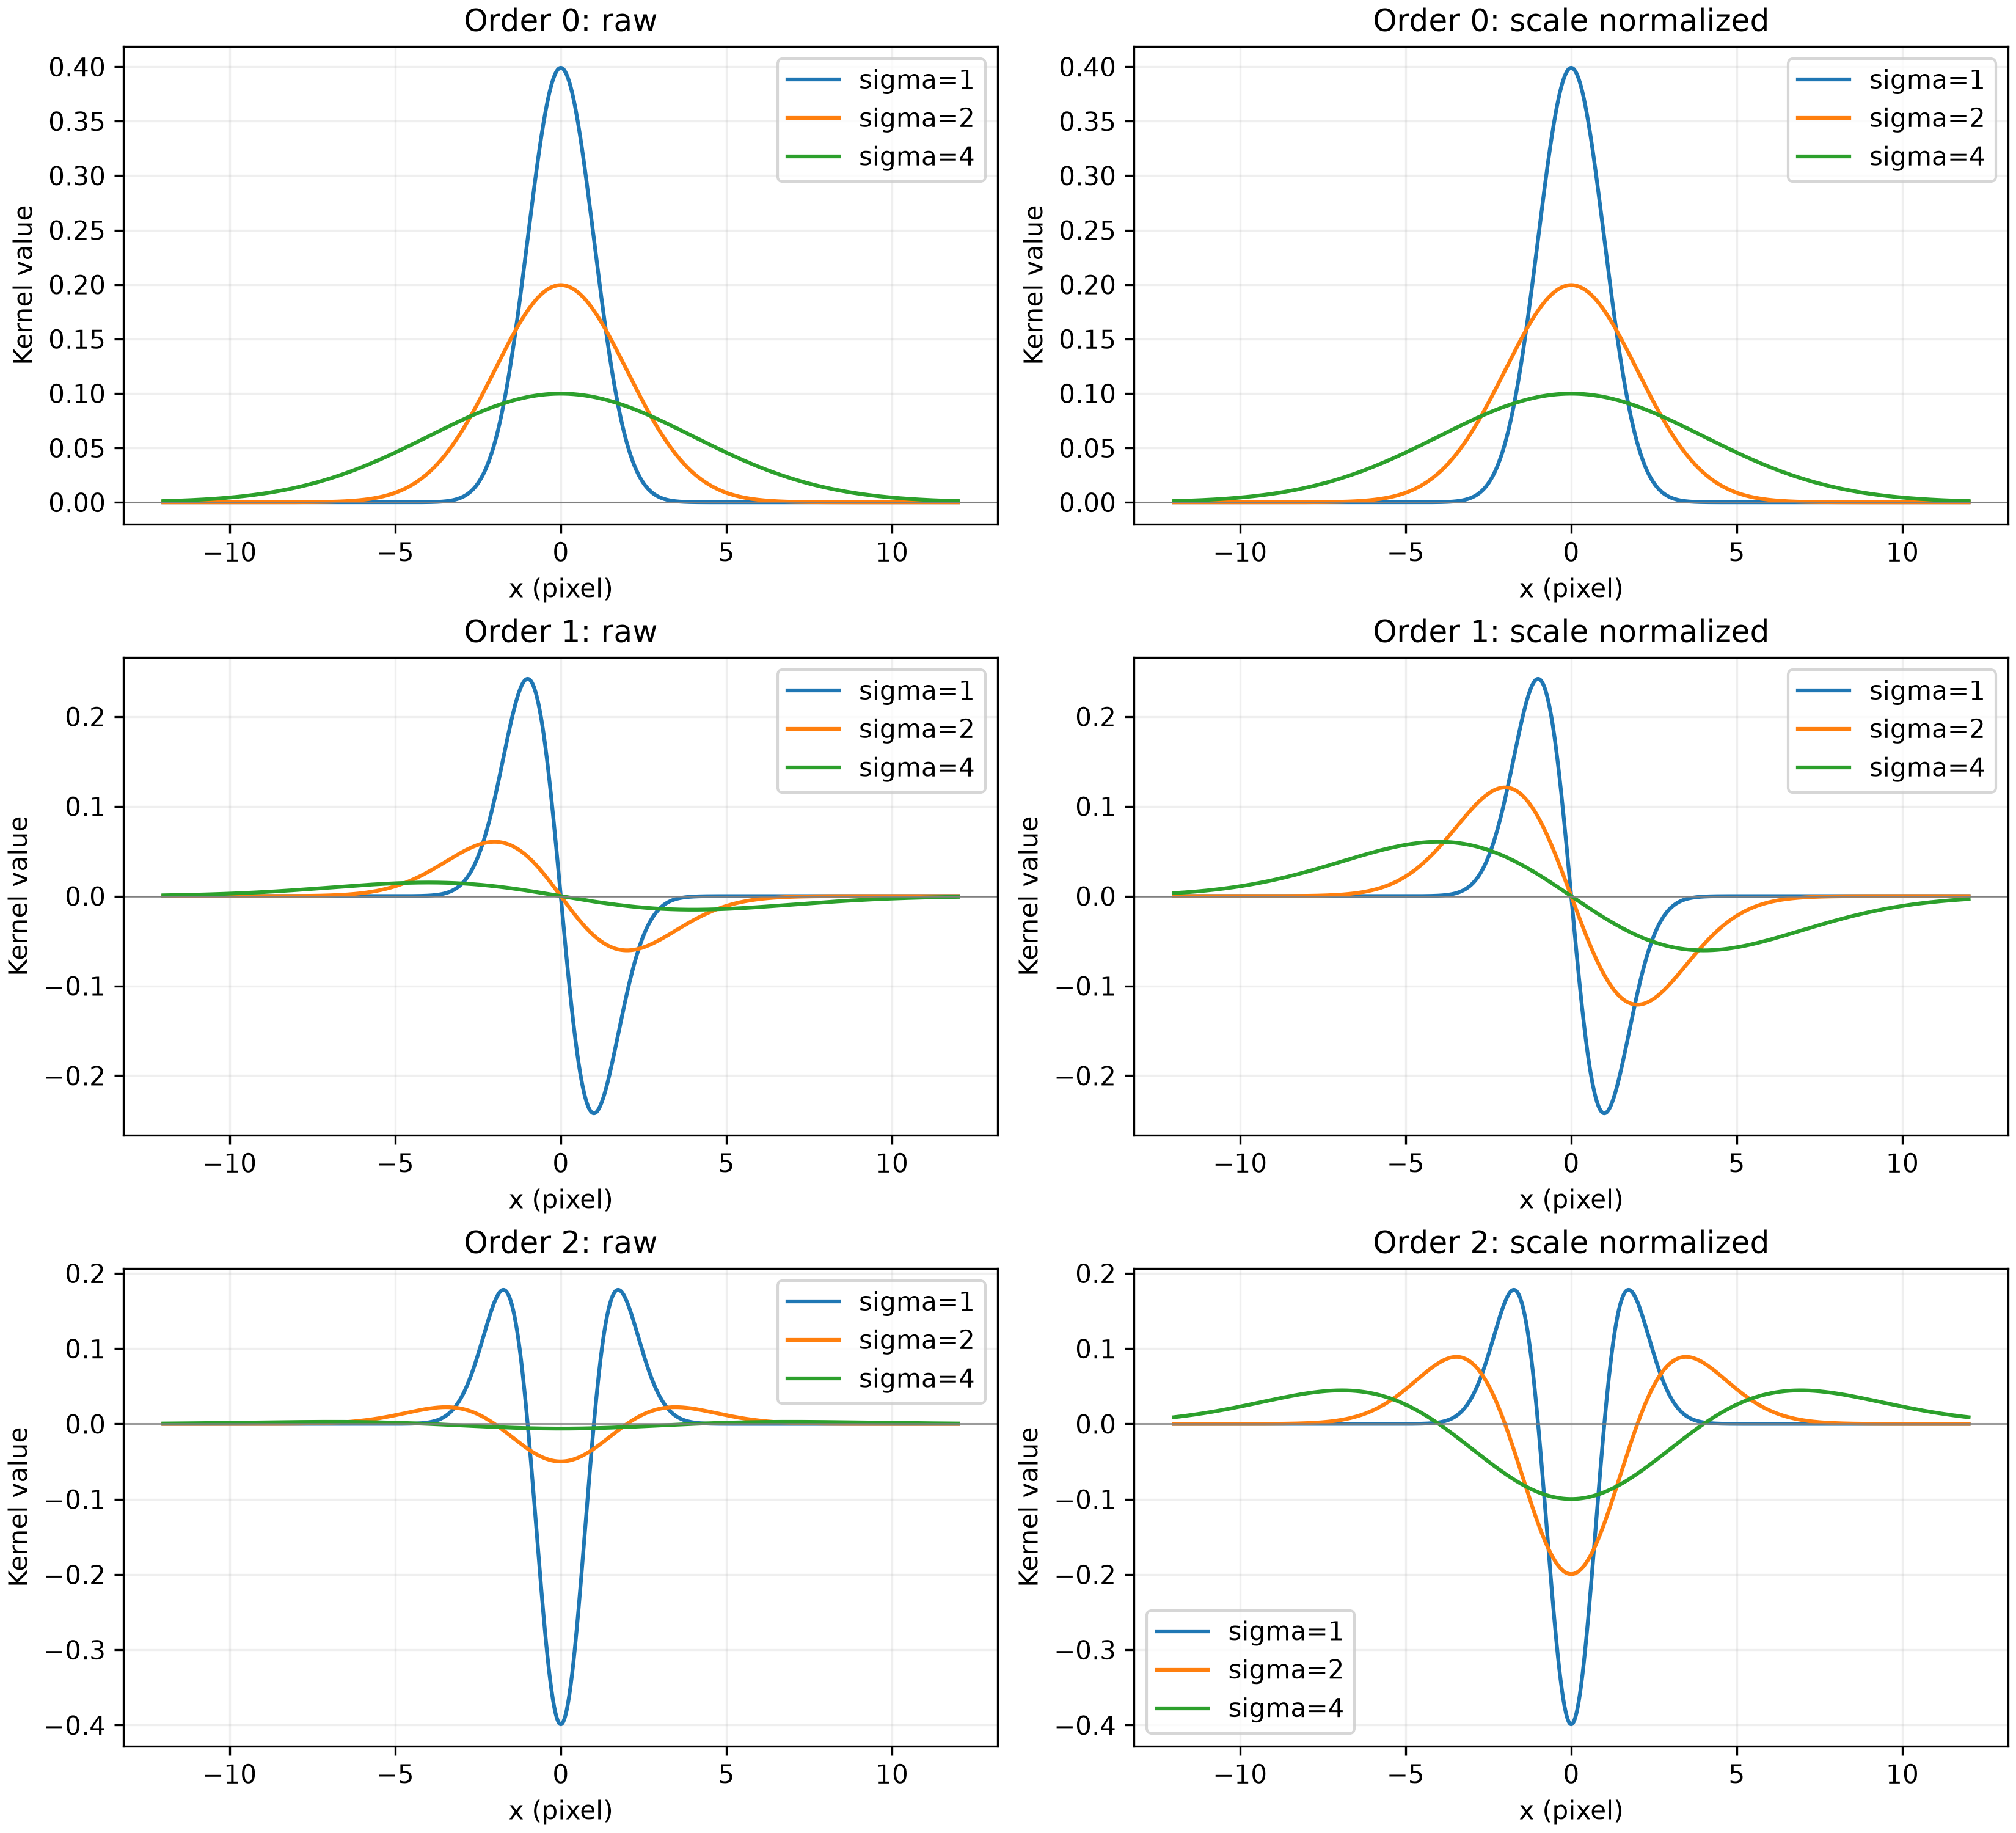
\includegraphics[width=0.90\textwidth]{figures/theory_gaussian_derivatives.png}
\caption{Minh họa giải tích Gaussian và đạo hàm bậc 1, 2 tại ba tỷ lệ. Cột trái là kernel thô, cột phải nhân $\sigma^n$ theo bậc đạo hàm. Đây là đồ thị tính từ công thức, không phải đầu ra thực nghiệm của Fiji.}
\label{fig:analytic_kernels}
\end{figure*}

\subsection{Scale-space: biểu diễn ảnh theo tỷ lệ}
Scale-space là họ ảnh $\{L(\cdot,\cdot;\sigma)\}_{\sigma>0}$, không chỉ là một ảnh đã làm mịn. Ở tỷ lệ nhỏ, các chi tiết mảnh có thể tạo đáp ứng nổi bật; ở tỷ lệ lớn, các nhóm chi tiết có thể được quan sát như một cấu trúc lớn hơn. Cùng một cảnh có thể cần nhiều tỷ lệ vì biên lớn, mạch nhỏ và cụm tế bào không có cùng kích thước \cite{witkin1983scale,lindeberg1994scale}.

\subsubsection{Tính bán nhóm}
Gaussian thỏa mãn
\begin{equation}
G_{\sigma_1}*G_{\sigma_2}
=G_{\sqrt{\sigma_1^2+\sigma_2^2}}.
\end{equation}
Do đó, nếu đã có ảnh tại $\sigma_1$ và muốn tới $\sigma_2>\sigma_1$, mức làm mịn bổ sung trong mô hình liên tục là $\sqrt{\sigma_2^2-\sigma_1^2}$. Hai lần làm mịn với $\sigma=2$ cho tỷ lệ tổng $\sqrt8$, không phải $\sigma=4$. Quan hệ này giải thích vì sao phải quản lý phương sai khi xây dựng nhiều mức tỷ lệ.

\subsubsection{Liên hệ với phương trình truyền nhiệt}
Đặt $t=\sigma^2$. Họ ảnh Gaussian giải phương trình
\begin{equation}
\frac{\partial L}{\partial t}=\frac12\nabla^2L,\qquad L(x,y;0)=I(x,y).
\end{equation}
Mô hình này làm giảm độ tương phản của các cấu trúc nhỏ dần theo $t$. Tính không tăng cường cực trị cục bộ là một cơ sở quan trọng của scale-space Gaussian; không nên suy diễn rằng mọi cấu trúc phát hiện trong ảnh 2D luôn giữ nguyên số lượng hay vị trí qua các tỷ lệ.

\subsubsection{Chọn lưới tỷ lệ}
Repo dùng $\Sigma=\{1,2,4,8\}$ cho đối chiếu cơ bản và lưới dày hơn $\{1,1.4,2,2.8,4,5.7,8\}$ cho Blobs. Lưới hình học cho khoảng cách tương đối gần nhau giữa các kích thước. Lưới thưa giảm thời gian, nhưng có thể bỏ lỡ cực trị theo tỷ lệ nằm giữa hai mức. Lưới dày tăng khả năng định vị kích thước, đồng thời tăng chi phí và số ứng viên cần khử trùng.

\subsection{Đạo hàm Gaussian bậc nhất}
Tính tuyến tính cho phép chuyển đạo hàm sang kernel:
\begin{equation}
L_x=I*\partial_xG_\sigma,\qquad L_y=I*\partial_yG_\sigma.
\end{equation}
Các kernel một chiều tương ứng là
\begin{align}
g'_\sigma(x)&=-\frac{x}{\sigma^2}g_\sigma(x),\\
G_{\sigma,x}(x,y)&=g'_\sigma(x)g_\sigma(y),\\
G_{\sigma,y}(x,y)&=g_\sigma(x)g'_\sigma(y).
\end{align}
Kernel bậc nhất là hàm lẻ, có tổng liên tục bằng 0. Vì vậy ảnh hằng phải cho đạo hàm gần 0; sai khác có hệ thống trên ảnh hằng là một dấu hiệu lỗi chuẩn hóa, đệm biên hoặc cài đặt.

$L_x$ đo biến thiên theo phương ngang nên thường nổi bật tại biên đứng; $L_y$ đo biến thiên theo phương dọc nên thường nổi bật tại biên ngang. Dấu đáp ứng cho biết hướng tăng hoặc giảm cường độ theo trục đã quy ước. Bản đồ có dấu cần được lưu dưới dạng số thực, thay vì chuyển về ảnh 8-bit trước khi đối chiếu.

\subsubsection{Ví dụ biên bước}
Xét biên đứng lý tưởng $I(x)=A\,H(x)$, trong đó $H$ là hàm bước. Sau làm mịn,
\begin{equation}
L(x;\sigma)=A\Phi(x/\sigma),\quad
L_x(x;\sigma)=\frac{A}{\sqrt{2\pi}\sigma}e^{-x^2/(2\sigma^2)}.
\end{equation}
Đạo hàm đạt cực đại ở vị trí biên $x=0$. Khi tăng $\sigma$, đỉnh đáp ứng thấp hơn và rộng hơn; điều này giải thích vì sao gradient lớn không tự động tạo ra một đường biên mảnh. Bước NMS trong Canny giữ lại cực đại theo phương gradient để cải thiện định vị.

\subsection{Gradient: cường độ và hướng biến thiên}
Vector gradient và độ lớn của nó là
\begin{equation}
\nabla L=\begin{bmatrix}L_x\\L_y\end{bmatrix},\quad
M=\sqrt{L_x^2+L_y^2},\quad
\theta=\operatorname{atan2}(L_y,L_x).
\end{equation}
Gradient chỉ theo phương tăng cường độ nhanh nhất; tiếp tuyến của biên lý tưởng vuông góc với gradient. Hàm atan2 sử dụng dấu của cả hai thành phần nên xác định đúng góc phần tư và xử lý trường hợp $L_x=0$ tốt hơn biểu thức $\arctan(L_y/L_x)$.

Độ lớn gradient là bất biến đối với việc quay hệ trục trong mô hình liên tục. Tuy nhiên, cài đặt trên lưới pixel, phép nội suy và lượng tử hóa hướng có thể tạo sai khác theo góc. Trong vùng đồng nhất, khi $M$ gần 0, hướng gradient trở nên nhạy với nhiễu và không nên được diễn giải như một hướng cấu trúc đáng tin cậy.

\subsection{Đạo hàm bậc hai và Laplacian}
Đạo hàm bậc hai một chiều có dạng
\begin{equation}
g''_\sigma(x)=\left(\frac{x^2}{\sigma^4}-\frac1{\sigma^2}\right)g_\sigma(x).
\end{equation}
Trong ảnh hai chiều,
\begin{align}
L_{xx}&=I*(g''_\sigma(x)g_\sigma(y)),\\
L_{yy}&=I*(g_\sigma(x)g''_\sigma(y)),\\
L_{xy}&=I*(g'_\sigma(x)g'_\sigma(y)).
\end{align}
Các đại lượng này đo sự thay đổi của độ dốc, cung cấp thông tin về độ cong mà đạo hàm bậc nhất chưa mô tả đầy đủ. $L_{xy}$ phản ánh sự tương tác giữa hai phương và cần thiết để phân tích các cấu trúc nghiêng.

Laplacian là tổng hai đạo hàm thuần:
\begin{equation}
\nabla^2L=L_{xx}+L_{yy}.
\end{equation}
Đây là một đại lượng vô hướng, hữu ích cho blob và phân tích điểm đổi dấu. Tuy nhiên, hai ma trận Hessian khác nhau có thể có cùng tổng trị riêng; Laplacian một mình không đủ phân biệt cấu trúc dạng đường, dạng đốm hay điểm yên ngựa.

\subsection{Ma trận Hessian và hình học cục bộ}
Khai triển Taylor của ảnh quanh điểm $\mathbf p$ theo độ lệch $\mathbf h$ cho
\begin{equation}
L(\mathbf p+\mathbf h)\approx
L(\mathbf p)+\nabla L^\top\mathbf h+
\frac12\mathbf h^\top\mathcal H\mathbf h,
\end{equation}
với
\begin{equation}
\mathcal H=
\begin{bmatrix}L_{xx}&L_{xy}\\L_{xy}&L_{yy}\end{bmatrix}.
\end{equation}
Do Hessian đối xứng, hai vector riêng có thể được chọn trực giao và trị riêng là số thực. Theo một vector đơn vị $\mathbf v$, đạo hàm bậc hai có hướng là $\mathbf v^\top\mathcal H\mathbf v$. Hai trị riêng chính là các độ cong cực trị của dạng toàn phương này:
\begin{equation}
\lambda_\pm=\frac{L_{xx}+L_{yy}}2
\pm\sqrt{\left(\frac{L_{xx}-L_{yy}}2\right)^2+L_{xy}^2}.
\end{equation}

\subsubsection{Ý nghĩa dấu và độ lớn}
Tại một cực đại sáng cục bộ, cả hai độ cong thường âm; tại cực tiểu tối, chúng thường dương. Với ridge sáng, độ cong ngang thân âm mạnh và độ cong dọc thân nhỏ; với rãnh tối, dấu độ cong ngang thân đảo lại. Trường hợp hai trị riêng trái dấu tương ứng hình học yên ngựa. Các mô tả này áp dụng cho đáp ứng cục bộ ở tỷ lệ đang khảo sát, không phải một bộ phân loại hoàn chỉnh chỉ dựa vào dấu.

Thứ tự trị riêng cần được ghi rõ: FeatureJ ở cấu hình đối chiếu dùng thứ tự đại số $\lambda_+\geq\lambda_-$; Frangi thường sắp theo $|\lambda_1|\leq|\lambda_2|$. Sắp xếp theo trị tuyệt đối không có nghĩa thay trị riêng bằng trị tuyệt đối: dấu vẫn phải được giữ để chọn ridge sáng hay tối.

\subsubsection{Ví dụ kiểm tra bằng ảnh đa thức}
Với $I(x,y)=ax^2+2bxy+cy^2+dx+ey+f$, ta có
\begin{equation}
\nabla I=\begin{bmatrix}2ax+2by+d\\2bx+2cy+e\end{bmatrix},
\quad
\mathcal H_I=\begin{bmatrix}2a&2b\\2b&2c\end{bmatrix}.
\end{equation}
Trong miền liên tục không biên, làm mịn thêm hằng số $\sigma^2(a+c)$ vào ảnh nhưng không đổi Hessian. Vì vậy ảnh đa thức là một ví dụ hữu ích để kiểm tra dấu, thứ tự trục và đáp ứng bậc hai. Trên ảnh hữu hạn, cần loại vùng chịu ảnh hưởng của đệm biên.

\subsection{Chuẩn hóa đạo hàm theo tỷ lệ}
Để so sánh đáp ứng giữa các tỷ lệ, đạo hàm tổng bậc $n$ được chuẩn hóa bởi
\begin{equation}
L_{x^my^k,\gamma}=\sigma^{(m+k)\gamma}L_{x^my^k},\quad n=m+k.
\end{equation}
Với $\gamma=1$, đạo hàm bậc nhất nhân $\sigma$ và đạo hàm bậc hai nhân $\sigma^2$ \cite{lindeberg1998feature}. Ví dụ biên bước cho $\sigma L_x(0;\sigma)=A/\sqrt{2\pi}$: biên độ chuẩn hóa tại đỉnh không còn giảm chỉ vì tăng $\sigma$.

Chuẩn hóa giúp so sánh cấu trúc ở nhiều kích thước, nhưng không đảm bảo mọi ảnh và mọi dạng đối tượng đều có cùng độ nhạy. Cần phân biệt hai loại phép đo: đối chiếu toán tử thô với FeatureJ phải dùng cùng cờ chuẩn hóa; phát hiện đa tỷ lệ có thể chủ động dùng đáp ứng chuẩn hóa. Chuẩn hóa hai lần sẽ tạo hệ số sai lệch phụ thuộc $\sigma$.

\subsection{Structure Tensor: tổng hợp định hướng trong lân cận}
Hessian dùng đạo hàm bậc hai tại một tỷ lệ. Structure Tensor tổng hợp tích các đạo hàm bậc nhất trong một vùng:
\begin{equation}
\mathcal S_{\sigma_d,\sigma_i}
=G_{\sigma_i}*
\begin{bmatrix}
L_x^2&L_xL_y\\L_xL_y&L_y^2
\end{bmatrix}_{\sigma_d}.
\end{equation}
$\sigma_d$ điều khiển tỷ lệ tính gradient, còn $\sigma_i$ điều khiển vùng tích phân hướng. Tăng $\sigma_i$ làm hướng ổn định hơn trong vùng nhiễu, nhưng cũng có thể gộp nhiều cấu trúc có hướng khác nhau.

Với mọi $\mathbf v$, $\mathbf v^\top\mathcal S\mathbf v$ là trung bình có trọng số của $(\mathbf v^\top\nabla L)^2$, nên $\mathcal S$ bán xác định dương. Hai trị riêng $\mu_1\geq\mu_2\geq0$ được diễn giải như sau: cả hai nhỏ biểu thị vùng gần đồng nhất; $\mu_1$ lớn và $\mu_2$ nhỏ biểu thị một hướng biến thiên ưu thế; cả hai lớn thường xuất hiện ở góc hoặc vùng kết cấu nhiều hướng.

\begin{equation}
C=\frac{\mu_1-\mu_2}{\mu_1+\mu_2+\epsilon}
\end{equation}
là một độ đo coherence thường dùng. $C$ cao chỉ hữu ích khi năng lượng gradient đủ lớn; vùng rất tối hoặc đồng nhất có thể tạo tỷ số thiếu ổn định nếu bỏ $\epsilon$. Vector riêng ứng với $\mu_1$ gần hướng pháp tuyến của cấu trúc dạng đường, còn hướng tiếp tuyến tương ứng phương còn lại. Vì tensor dùng tích gradient, đảo tương phản không làm đổi nó như đối với dấu Hessian.

\subsection{Từ đặc trưng vi phân đến ba bài toán phát hiện}
\subsubsection{Biên: gradient, NMS và hysteresis}
Canny bắt đầu bằng đạo hàm của ảnh làm mịn, tính $M,\theta$, rồi thực hiện NMS và phân ngưỡng kép \cite{canny1986computational}. NMS giữ các điểm có $M$ cực đại cục bộ theo pháp tuyến biên. Hysteresis giữ điểm mạnh $M\geq T_h$ và điểm yếu $T_l\leq M<T_h$ nếu có đường liên thông tới điểm mạnh. Ngưỡng quá thấp giữ nhiều kết cấu nền; ngưỡng quá cao bỏ sót biên có tương phản yếu.

Gradient mạnh phản ánh thay đổi cường độ, còn nhãn đường biên của con người thường gắn với đối tượng. Vì thế biên do bóng, nhiễu kết cấu hoặc vân nền có thể bị thuật toán giữ lại nhưng không được người gán nhãn xem là đường bao cần thiết. Đây là một nguyên nhân khiến đối chiếu số học tốt chưa kéo theo F1 phát hiện cao.

\subsubsection{Ridge: phân tích độ cong ngang và dọc}
Một mô hình ridge sáng thẳng là $I(x,y)=A\exp[-x^2/(2s^2)]$, không đổi theo $y$. Gần tâm ridge, $L_{xx}$ âm và $L_{yy}$ gần 0; độ cong lớn nằm theo phương ngang thân. Với ridge tối trên nền sáng, dấu đảo lại. Mạch máu trong ảnh DRIVE được xem là cấu trúc tối, nên lựa chọn cực tính phải phù hợp.

Frangi dùng tỷ số $R_B=|\lambda_1|/(|\lambda_2|+\epsilon)$ và độ mạnh $S=\sqrt{\lambda_1^2+\lambda_2^2}$ sau chuẩn hóa tỷ lệ \cite{frangi1998multiscale}. $R_B$ nhỏ gợi ý cấu trúc dài; thừa số theo $S$ giảm đáp ứng ở nền ít cấu trúc. Lấy cực đại theo $\sigma$ giúp tổng hợp các mạch khác độ rộng, song còn cần ngưỡng, mặt nạ FOV và cách đánh giá vùng phân đoạn.

\subsubsection{Blob: cực trị đồng thời theo vị trí và tỷ lệ}
Đáp ứng $R(x,y,\sigma)=\sigma^2|\nabla^2L|$ được tìm cực đại theo cả không gian và tỷ lệ. Dấu của Laplacian trước phép lấy trị tuyệt đối giúp chọn blob sáng hoặc tối. Nếu chỉ tìm cực đại 2D độc lập ở từng mức, cùng một đối tượng có thể được đếm nhiều lần.

Với blob Gaussian lý tưởng $I=A\exp[-(x^2+y^2)/(2s^2)]$, tại tâm ta có
\begin{equation}
\sigma^2|\nabla^2L(0,0;\sigma)|
=\frac{2As^2\sigma^2}{(s^2+\sigma^2)^2}.
\end{equation}
Biểu thức đạt cực đại tại $\sigma=s$, cho một ví dụ giải tích về lựa chọn tỷ lệ đặc trưng. Quy ước $R\approx\sqrt2\sigma$ thường dùng để vẽ vòng tròn biểu diễn blob trong 2D; đây là ánh xạ kích thước theo mô hình, không phải đẳng thức bán kính thật cho mọi dạng tế bào.


\begin{figure}[htbp]
\centering
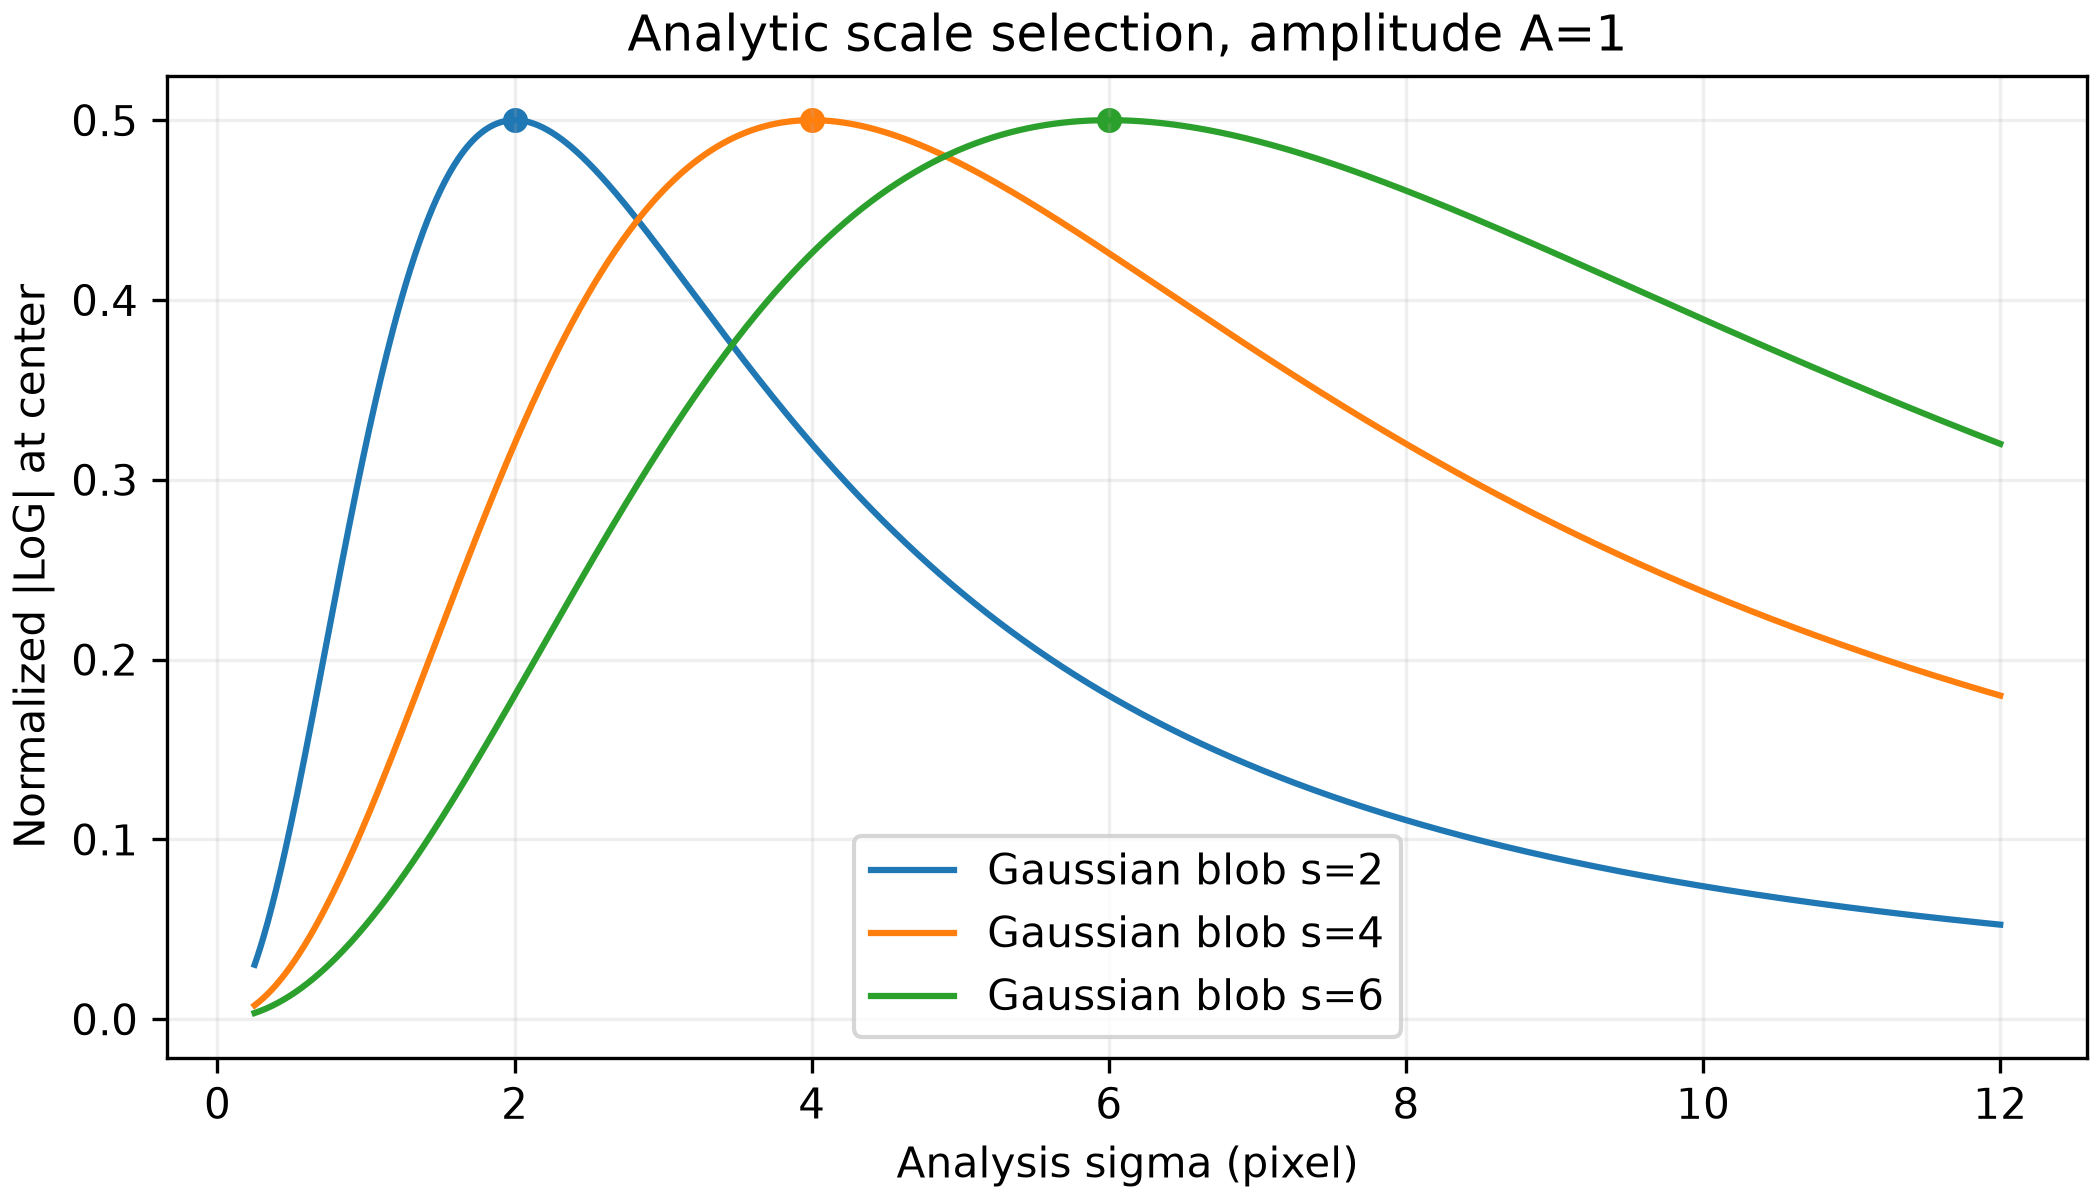
\includegraphics[width=\columnwidth]{figures/theory_blob_scale_selection.png}
\caption{Chọn tỷ lệ trên mô hình blob Gaussian biên độ 1: đáp ứng LoG chuẩn hóa tại tâm đạt cực đại khi $\sigma=s$. Đồ thị là ví dụ giải tích để giải thích nguyên lý chọn kích thước.}
\label{fig:analytic_blob_scale}
\end{figure}

\subsection{Tổng hợp ý nghĩa các bản đồ}
\begin{table*}[t]
\centering
\caption{Vai trò của các đại lượng vi phân và điểm cần lưu ý khi diễn giải}
\begin{tabularx}{\textwidth}{lXX}
\toprule
Đại lượng & Thông tin chính & Giới hạn khi sử dụng\\
\midrule
$L$ & Cường độ ở tỷ lệ $\sigma$ & Làm mịn mạnh có thể mất chi tiết nhỏ\\
$L_x,L_y$ & Biến thiên có hướng và có dấu & Phụ thuộc trục và quy ước tích chập\\
$\|\nabla L\|$ & Mức biến thiên tổng hợp & Biên mạnh có thể là kết cấu nền\\
$L_{xx},L_{yy},L_{xy}$ & Độ cong cục bộ & Nhạy với rời rạc hóa và nhiễu\\
$\mathcal H,\lambda_1,\lambda_2$ & Hình học ridge/blob, hướng độ cong & Phải thống nhất thứ tự và cực tính\\
$\sigma^2\nabla^2L$ & Đáp ứng blob chuẩn hóa & Cần cực trị theo tỷ lệ và khử trùng\\
$\mathcal S,\mu_1,\mu_2$ & Năng lượng, hướng biến thiên trong vùng & Coherence cao cần đi kèm năng lượng đủ lớn\\
\bottomrule
\end{tabularx}
\end{table*}
Các bản đồ trên tạo một chuỗi phân tích: Gaussian xác định tỷ lệ quan sát; đạo hàm đo biến thiên; gradient, Hessian và tensor cô đọng thông tin; bộ dò cùng bước hậu xử lý chuyển thông tin liên tục thành biên, vùng mạch hoặc danh sách blob.


\section{Chương 3: Khảo Sát Nền Tảng Tham Chiếu FeatureJ / Fiji}

\subsection{Kiến Trúc Module FeatureJ và Gói Thư Viện ImageScience}
Plugin \textbf{FeatureJ} là tập công cụ ImageJ để trích xuất đặc trưng ảnh; trong Fiji, có thể cài qua update site ImageScience \cite{meijeringFeatureJ}. Các thao tác Derivatives, Edges, Hessian và Structure cung cấp các bản đồ dùng trong đối chiếu. Phần triển khai tham chiếu được đóng gói cùng thư viện ImageScience.

Kiến trúc bên trong của ImageScience bao gồm các lớp đối tượng chính:
\begin{itemize}
    \item \texttt{imagescience.image.Image}: Cấu trúc dữ liệu ImageScience hỗ trợ ảnh nhiều chiều (đến 5D) và cho phép xử lý dữ liệu dấu chấm động; lớp này giao tiếp với đối tượng ảnh ImageJ.
    \item \texttt{imagescience.feature.Differentiator}: Trái tim của toàn bộ giải thuật vi phân. Lớp này chịu trách nhiệm sinh hạt nhân Gaussian 1D, thực hiện tích chập tách rời theo các trục tọa độ không gian và áp dụng các điều kiện biên.
    \item \texttt{imagescience.feature.Hessian}: Tính toán các đạo hàm bậc 2 $L_{xx}, L_{yy}, L_{xy}$, xây dựng ma trận Hessian tại từng pixel và tính toán các trị riêng $\lambda_1, \lambda_2$ bằng phép chiếu giải tích.
    \item \texttt{imagescience.feature.Structure}: Tính toán Ten-xơ cấu trúc với cặp tỷ lệ vi phân - tích phân $(\sigma_d, \sigma_i)$ và trích xuất độ định hướng cục bộ (\textit{coherence}).
\end{itemize}

\subsection{Các quy ước tham số cần đối chiếu}
Cấu hình và các bộ xuất trong repo xác định những quy ước dùng cho lần đối chiếu này. Bảng sau mô tả cấu hình thực nghiệm của dự án; không suy rộng chúng thành mặc định của mọi phiên bản FeatureJ \cite{xlaRepository}.

\begin{table*}[t]
\caption{Ánh xạ tham số dùng trong cấu hình đối chiếu của dự án}
\centering
\resizebox{\textwidth}{!}{\begin{tabular}{lll}
\toprule
\textbf{Tham số hệ thống} & \textbf{Quy ước FeatureJ} & \textbf{Cài đặt Python Core} \\
\midrule
Bán kính cắt kernel bậc 0 & $r = \lceil 3.0\sigma \rceil$ & $r = \lceil 3.0\sigma \rceil$ (\texttt{kernel\_k.gauss=3.0}) \\
Bán kính cắt kernel bậc 1, 2 & $r = \lceil 4.0\sigma \rceil$ & $r = \lceil 4.0\sigma \rceil$ (\texttt{kernel\_k.lx=4.0}) \\
Điều kiện biên không gian & \texttt{mirror} (không lặp biên) & \texttt{mode='reflect'} (NumPy) \\
Thứ tự trị riêng Hessian & Đại số ($\lambda_1 \ge \lambda_2$) & Đại số (\texttt{algebraic}) \\
Chuẩn hóa biên độ $\sigma^\gamma$ & Thô (\texttt{normalized=false}) & Thô theo FeatureJ / Chuẩn hóa khi dò \\
Biểu diễn trao đổi & TIFF float32 & float64 tính toán, TIFF float32 \\
Định dạng file xuất đĩa & TIFF 32-bit Float & TIFF 32-bit Float (\texttt{tifffile}) \\
\bottomrule
\end{tabular}}
\label{tab:featurej_mapping}
\end{table*}

\subsection{Phân Tích Bản Chất Khác Biệt Rời Rạc Hóa: Taylor Moments vs. Continuous Sampling}
Một quan sát trong quá trình thẩm định là sai khác có hệ thống giữa các toán tử bậc cao của Python Core và FeatureJ. Các phép đo phù hợp với khác biệt trong cách xây dựng kernel rời rạc; đây là giải thích cho sai số quan sát được, không phải khẳng định rằng hai phương pháp luôn có cùng quy ước nội bộ:
\begin{itemize}
    \item \textbf{Phương pháp FeatureJ:} Các bản đồ xuất từ phiên bản được khảo sát có sai khác biên độ nhỏ so với Python, rõ hơn ở đạo hàm bậc hai. Phép đo không cho thấy sai khác hình học lớn; tuy nhiên không thể suy ra toàn bộ chi tiết nội bộ chỉ từ các bản đồ đầu ra.
    \item \textbf{Phương pháp Python Core (Discrete Taylor Conditions):} Bộ sinh kernel áp dụng các ràng buộc moment Taylor rời rạc theo cấu hình của dự án \cite{xlaRepository}. Các hệ số lọc được xác định để moment bậc $0,1,2$ tiến tới giá trị mục tiêu trên lưới rời rạc:
    \begin{equation}
    \sum_{n=-r}^r n^p g^{(m)}[n] = (-1)^m m! \cdot \delta_{p, m}
    \end{equation}
\end{itemize}
Trong bộ dữ liệu kiểm tra, sai số tương đối trung bình của các toán tử bậc hai xấp xỉ $0.3$--$0.4\%$, trong khi Pearson vẫn lớn hơn $0.9999$. Vì vậy báo cáo trình bày riêng sai số biên độ và tương quan hình dạng, không diễn giải tương quan cao thành đồng nhất số học.

\subsection{Kiến trúc tổng quan của hệ thống}
Hình~\ref{fig:system_architecture} mô tả luồng dữ liệu từ ảnh đầu vào và cấu hình chung đến hai nhánh tính toán và hai tầng đánh giá. Cùng một ảnh và tỷ lệ được đưa vào nhân NumPy và bộ tham chiếu Fiji/FeatureJ. Các phép xử lý cần thống nhất kiểu dữ liệu, bậc đạo hàm, đơn vị, quy ước chuẩn hóa và cách loại bỏ vùng biên trước khi đối chiếu.

\begin{figure*}[t]
\centering
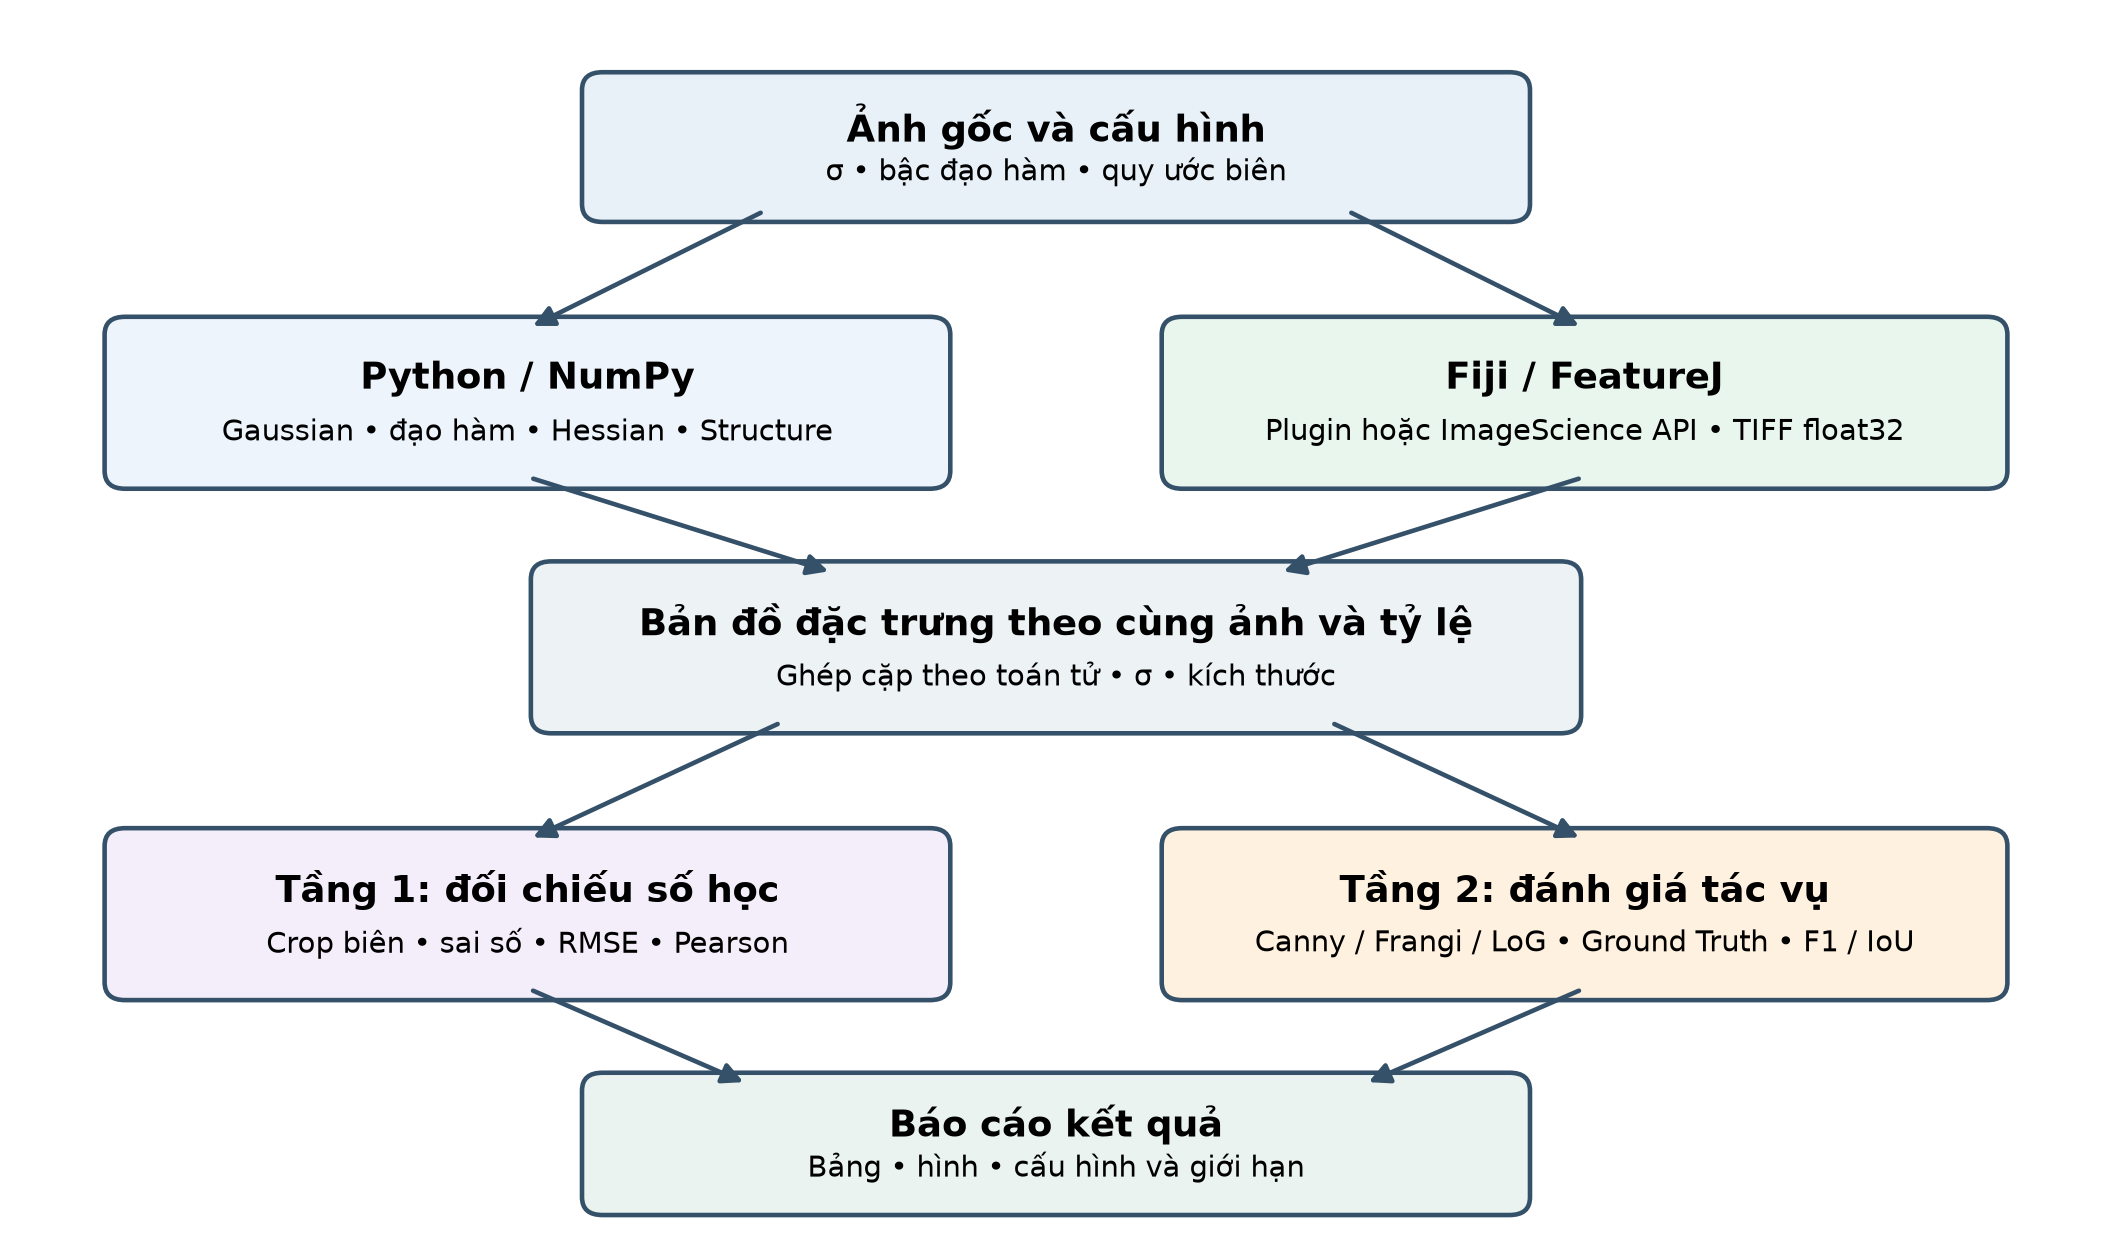
\includegraphics[width=0.94\textwidth]{figures/system_architecture.png}
\caption{Kiến trúc xử lý và đánh giá của dự án: hai nhánh tính bản đồ đặc trưng, đối chiếu số học ở Tầng 1 và đánh giá tác vụ với Ground Truth ở Tầng 2. Sơ đồ mô tả quy trình tổng quát; bộ chạy mẫu mới chỉ bao gồm ba ảnh và sáu toán tử.}
\label{fig:system_architecture}
\end{figure*}

Ở Tầng 1, các bản đồ cùng ảnh, toán tử và tỷ lệ được ghép cặp để tính sai số và Pearson trên vùng hợp lệ. Ở Tầng 2, các bản đồ đặc trưng đi qua thuật toán phát hiện tương ứng rồi so với nhãn tham chiếu; F1 và IoU phản ánh kết quả tác vụ theo giao thức đã chọn. Chẳng hạn, nhánh Fiji của phép so sánh Canny công bằng cung cấp $L_x,L_y$ rồi dùng cùng bước hậu xử lý Python; kết quả FeatureJ Edges được báo cáo riêng. Sơ đồ không hàm ý rằng phiên GUI bổ sung đã chạy lại toàn bộ benchmark của nhóm.

\subsection{Vai trò của Fiji/FeatureJ và mã nguồn Python trong báo cáo}
Fiji là môi trường xử lý ảnh dựa trên ImageJ; FeatureJ là bộ plugin cung cấp các phép trích xuất đặc trưng vi phân \cite{meijeringFeatureJ}. Trong đề tài này, Fiji/FeatureJ cung cấp một bộ cài đặt độc lập để kiểm tra nhân NumPy. Repo cung cấp nhân tính toán, dữ liệu, cấu hình, macro và bộ đánh giá. Hai thành phần cần được nối bằng cùng ảnh đầu vào và cùng quy ước tham số để phép so sánh có ý nghĩa.

Tài liệu yeucau.md của repo yêu cầu workflow Fiji, cài đặt thuật toán và đối chiếu định lượng giữa công cụ với code nhóm; không quy định từng thành viên phải tự chạy lại toàn bộ dữ liệu. Người viết báo cáo có thể tổng hợp kết quả nhóm đã tạo nếu chỉ rõ nguồn. Để bảo đảm hiểu workflow và có minh chứng thực hành, phương án trong bản báo cáo này là chạy lại một tập nhỏ, đồng thời dùng CSV của nhóm cho các bảng tổng hợp. Các kết quả nhóm có sẵn và kết quả mới phải có nhật ký riêng.

\subsection{Chuẩn bị môi trường và kiểm tra đầu vào}
\subsubsection{Fiji và plugin}
Tải Fiji từ nguồn chính thức, giải nén vào thư mục có quyền ghi, mở chương trình rồi dùng trình cập nhật để bật update site ImageScience. Sau khi cập nhật và khởi động lại, kiểm tra các lệnh FeatureJ Derivatives, Edges, Laplacian, Hessian và Structure xuất hiện. Không chỉ kiểm tra tên plugin: cần mở thử một ảnh xám và xác nhận một phép đạo hàm chạy thành công.

Ghi lại phiên bản Fiji/ImageJ, Java, FeatureJ và ImageScience trong nhật ký chạy. Các tên cửa sổ đầu ra và lựa chọn của hộp thoại có thể thay đổi theo phiên bản; công cụ Macro Recorder của ImageJ giúp kiểm tra chuỗi tùy chọn thực sự được gửi tới plugin trên máy đang dùng.

\subsubsection{Môi trường Python}
Repo sử dụng NumPy trong nhân toán học; Pillow để đọc PNG, tifffile để trao đổi TIFF float, PyYAML để đọc cấu hình, SciPy trong một số bước đánh giá và Matplotlib để vẽ. Cần tạo môi trường riêng, cài theo requirements.txt của repo, rồi ghi lại phiên bản thực tế thay vì coi danh sách phiên bản đề xuất trong README là phiên bản máy đã cài.

Mọi lệnh chạy nên bắt đầu từ thư mục gốc của repo, nơi chứa config.yaml, data và src. Kiểm tra ảnh cùng nhãn đã có trước khi chạy. Một repo chỉ có mã mà thiếu dữ liệu hoặc kho TIFF tham chiếu sẽ chưa đủ để tái lập toàn bộ bảng.

\subsection{Thí nghiệm mẫu đề xuất}
Chọn ba ảnh đại diện: bsds\_01 cho biên, drive\_01 cho cấu trúc mạch và blob\_01 cho đốm tổng hợp. Dùng $\sigma=\{1,2,4,8\}$ và giữ nguyên kích thước ảnh. Bộ chạy mẫu kèm báo cáo xuất $L,L_x,L_y,L_{xx},L_{xy},L_{yy}$ cho mỗi ảnh và tỷ lệ: tổng cộng $3\times4\times6=72$ bản đồ trên mỗi nhánh.

Tập này dùng để kiểm tra thao tác, đọc bản đồ và đo sai khác toán tử. Nó không thay thế benchmark 25 ảnh và không đủ để đưa ra kết luận tổng quát về ba bộ dò. Khi cần minh họa độ khó của dữ liệu sinh học, mở thêm blob\_05 và đối chiếu với kết quả tổng hợp trong CSV nhóm.

\subsubsection{Quy trình thao tác trên một ảnh}
\begin{enumerate}
\item Mở đúng PNG từ data/raw và ghi lại tên file. Không dùng ảnh chụp màn hình hoặc bản JPEG có nén thay cho ảnh gốc.
\item Đặt đơn vị không gian là pixel, sau đó chuyển ảnh làm việc sang 32-bit. Không thay đổi dải cường độ độc lập cho từng nhánh.
\item Chạy FeatureJ Derivatives tại cùng $\sigma$: bậc $(0,0)$ cho Gaussian, $(1,0)$ cho $L_x$, $(0,1)$ cho $L_y$, $(2,0)$ cho $L_{xx}$, $(1,1)$ cho $L_{xy}$ và $(0,2)$ cho $L_{yy}$. Với ảnh một lát, bậc theo $z$ bằng 0.
\item Lưu mỗi bản đồ bằng TIFF 32-bit. Tên file ghi rõ ảnh, toán tử và $\sigma$; không ghi đè ảnh gốc.
\item Chạy nhân Python trên cùng PNG và xuất cùng sáu toán tử. Chỉ đối chiếu các cặp đã khớp ảnh, kích thước, toán tử và tỷ lệ.
\item Loại vùng biên theo bán kính hỗ trợ kernel trước khi tính sai số. Lưu cả giá trị số và một hình ghép để đọc trực quan.
\end{enumerate}

\subsection{Phân biệt bản đồ gradient và đầu ra biên}
Trong FeatureJ Edges, tính gradient, NMS và phân ngưỡng là các lựa chọn liên quan nhưng khác nhau. Gradient chưa NMS thường tạo dải đáp ứng rộng; bản đồ sau NMS mảnh hơn; ảnh sau hysteresis là kết quả nhị phân. Nếu lấy một ảnh nhị phân so với gradient float, sai khác sẽ chủ yếu phản ánh khác tầng xử lý.

Ở nhánh BSDS dùng cho so sánh công bằng trong repo, Fiji xuất $L_x,L_y$; Python nhân $\sigma$ và đưa chúng qua cùng detect\_canny như nhánh NumPy. Các ngưỡng được chọn trên Python rồi giữ cố định khi áp cho Fiji. FeatureJ Edges có NMS nội bộ là tham chiếu riêng với ngưỡng tuyệt đối riêng; F1 của nó được báo cáo ở cột riêng \cite{xlaRepository}. Do đó, cột mang tên Fiji trong bảng fair không đồng nghĩa toàn bộ pipeline Canny được thực thi trong plugin.

\subsection{Hessian, Structure Tensor và cực tính}
Khi xuất Hessian để đối chiếu, chọn hai trị riêng lớn nhất/nhỏ nhất theo thứ tự đại số, giữ nguyên dấu. Chỉ sắp theo độ lớn khi bước Frangi yêu cầu. Đối với ảnh DRIVE có mạch tối, độ cong mạnh ngang mạch là dương theo quy ước cường độ của ảnh; dùng tiêu chí ridge sáng sẽ làm mất phần đáp ứng cần quan tâm.

Với Structure Tensor, đặt riêng tỷ lệ vi phân và tích phân theo config.yaml: $(1,3)$ và $(2,6)$. Ghi cả hai vào tên file. Không dùng nhầm $\sigma_i$ làm tỷ lệ tính gradient, vì khi đó tensor vẫn có hình dạng hợp lý nhưng không còn là cùng phép đo với nhánh Python.

\subsection{Các nguồn tham chiếu và nguồn gốc đầu ra}
Bộ 220 TIFF của Java Exporter gọi ImageScience được dùng cho Tier 1. Bộ outputs/fiji của workflow macro phục vụ minh chứng công cụ và Tier 2. Theo README hiện hành, bộ macro gồm 423 TIFF trong phạm vi macro hợp nhất và 12 TIFF edge cũ được giữ lại, tổng 435 TIFF. Vì vậy không mô tả 435 file như sản phẩm của một lần chạy mới duy nhất nếu chưa có nhật ký xác nhận \cite{xlaRepository}.

Macro hiện hành batch\_process.ijm đọc config.yaml và bỏ qua một số file đầu ra đã tồn tại. Cơ chế này hữu ích để chạy tiếp, nhưng việc nhấn Run rồi thấy kết thúc không chứng minh mọi file vừa được tính lại. Khi cần đo thời gian hoặc tạo minh chứng mới, dùng thư mục đầu ra thí nghiệm riêng và lưu danh sách file được tạo trong lần chạy đó.

\subsection{Minh chứng cần thu thập cho báo cáo và bảo vệ}
\begin{table*}[t]
\centering
\caption{Minh chứng thực hành và câu hỏi mà mỗi minh chứng trả lời}
\begin{tabularx}{\textwidth}{lXX}
\toprule
Minh chứng & Nội dung cần ghi & Ý nghĩa\\
\midrule
Cấu hình phần mềm & Phiên bản, update site, lệnh FeatureJ & Xác nhận đúng môi trường tham chiếu\\
Ảnh gốc và metadata & Tên, kích thước, kiểu dữ liệu, đơn vị pixel & Xác nhận hai nhánh dùng cùng đầu vào\\
Hộp thoại lọc & Toán tử, bậc đạo hàm, $\sigma$, lựa chọn trị riêng & Cho phép tái lập phép đo\\
TIFF float và CSV & Bản đồ số gốc, sai số sau crop, trạng thái thiếu file & Cho phép kiểm tra định lượng\\
Hình ghép & Ảnh gốc, Python, Fiji, sai khác cùng thang màu & Giúp đọc vị trí và dạng sai khác\\
Nhật ký & Thời gian, lệnh, nguồn dữ liệu nhóm hay lần chạy mới & Phân biệt tái lập với tổng hợp\\
\bottomrule
\end{tabularx}
\end{table*}
Ảnh chụp giao diện chứng minh thao tác và cấu hình, nhưng không thay cho TIFF/CSV trong đối chiếu số học. Một hình đẹp sau tự động giãn tương phản cũng không chứng minh biên độ hai bản đồ bằng nhau; cần thang hiển thị chung và phép đo trên dữ liệu gốc.


\section{Chương 4: Thiết Kế và Cài Đặt Hệ Thống Python Core (From Scratch)}

\subsection{Triết Lý Thiết Kế và Kiến Trúc Mô-đun Hệ Thống}
Trong phạm vi \texttt{src/core/}, các toán tử tích chập, đạo hàm, Hessian, ten-xơ cấu trúc và bộ dò đặc trưng được cài đặt bằng NumPy. Nhân này không gọi các phép lọc OpenCV như \texttt{cv2.filter2D}/\texttt{cv2.Canny} hoặc bộ lọc Gaussian của SciPy; các thư viện ngoài lõi được dùng trong một số tiện ích kiểm thử và đánh giá.

Kiến trúc mã nguồn được phân tầng rõ ràng trong gói \texttt{src/core/}:
\begin{itemize}
    \item \texttt{src/config.py}: Trung tâm cấu hình tham số toàn cục. Định nghĩa chuẩn hóa các siêu tham số hệ thống: dãy tỷ lệ chuẩn $\sigma \in \{1.0, 2.0, 4.0, 8.0\}$, các cặp tỷ lệ vi phân - tích phân $(\sigma_d, \sigma_i) \in \{(1.0, 3.0), (2.0, 6.0)\}$ cho Ten-xơ cấu trúc, hệ số bán kính cắt hạt nhân theo bậc vi phân, và tiêu chuẩn định dạng dữ liệu (tính toán nội suy \texttt{float64}, xuất ảnh TIFF \texttt{float32}).
    \item \texttt{src/core/kernel.py}: Chịu trách nhiệm sinh các hạt nhân (kernel) Gaussian 1D cho các bậc đạo hàm $0, 1, 2$, tuân thủ nghiệm giải tích và điều kiện bảo toàn moment rời rạc.
    \item \texttt{src/core/convolution.py}: Thực thi tích chập 1D tách trục (\textit{Separable 1D Convolution}) kết hợp cơ chế phản xạ đối xứng qua gương (\textit{mirror reflection}).
    \item \texttt{src/core/derivatives.py}: Cung cấp giao diện tính toán các toán tử đạo hàm không gian: $L$ (làm mịn), $L_x, L_y$ (đạo hàm bậc nhất), $L_{xx}, L_{yy}, L_{xy}$ (đạo hàm bậc hai), độ lớn gradient $\|\nabla L\|$, và toán tử Laplace $\nabla^2 L$.
    \item \texttt{src/core/hessian.py}: Xây dựng ma trận Hessian và giải bài toán trị riêng 2D bằng công thức nghiệm giải tích khép kín, phân loại cấu trúc theo thứ tự đại số $\lambda_1 \ge \lambda_2$.
    \item \texttt{src/core/structure\_tensor.py}: Tính toán Ten-xơ cấu trúc hai tỷ lệ, trích xuất các trị riêng $\mu_1, \mu_2$, hướng cấu trúc cục bộ và độ kết hợp phương hướng (\textit{Coherence}).
    \item \texttt{src/core/detectors.py}: Tích hợp 3 bộ phát hiện đặc trưng cấp cao: Canny Edge Detector (với triệt tiêu không cực đại 8 hướng và loang liên thông BFS Hysteresis), Frangi Vesselness Filter (dò mạch máu đa tỷ lệ), và LoG Blob Detector (dò đốm 3D Scale-Space Extrema).
\end{itemize}

\subsection{Cơ Sở Rời Rạc Hóa và Bảo Toàn Taylor Discrete Moments}
Trong không gian liên tục $\mathbb{R}$, hàm mật độ Gaussian 1D và các đạo hàm bậc 1, bậc 2 của nó được xác định bởi:
\begin{align}
g(x; \sigma) &= \frac{1}{\sqrt{2\pi}\sigma} \exp\left(-\frac{x^2}{2\sigma^2}\right) \label{eq:gauss0} \\
g'(x; \sigma) &= -\frac{x}{\sigma^2} g(x; \sigma) \label{eq:gauss1} \\
g''(x; \sigma) &= \frac{x^2 - \sigma^2}{\sigma^4} g(x; \sigma) \label{eq:gauss2}
\end{align}
Nếu chỉ đơn thuần lấy mẫu các hàm liên tục trên tại các điểm tọa độ nguyên $x \in \mathbb{Z}$ và cắt cụt trong cửa sổ $[-r, r]$, trên lưới rời rạc tổng trọng số sẽ không bảo toàn năng lượng và gây ra sai số làm lệch độ dốc cục bộ.

Để xử lý sai khác do rời rạc hóa, bộ sinh kernel của dự án áp dụng các ràng buộc moment Taylor cho tín hiệu ảnh $I(x)$ quanh điểm $x_0$ \cite{xlaRepository}:
\begin{equation}
I(x_0 - n) = I(x_0) - n I'(x_0) + \frac{n^2}{2} I''(x_0) - \frac{n^3}{6} I^{(3)}(x_0) + \dots
\end{equation}
Khi thực hiện tích chập rời rạc $(I * h)[x_0] = \sum_{n=-r}^r h[n] I(x_0 - n)$, ta có:
\begin{align}
(I * h)[x_0] &= I(x_0) \sum_{n=-r}^r h[n] - I'(x_0) \sum_{n=-r}^r n h[n] \nonumber \\
&\quad + \frac{I''(x_0)}{2} \sum_{n=-r}^r n^2 h[n] - \dots
\end{align}
Để phép chập tái lập hoàn hảo đạo hàm bậc tương ứng của tín hiệu mà không bị nhiễu bởi các bậc khác, các hạt nhân rời rạc $g_0, g_1, g_2$ trong \texttt{kernel.py} được chuẩn hóa để thỏa mãn hệ phương trình moment nghiêm ngặt:
\begin{itemize}
    \item \textbf{Hạt nhân bậc 0 ($g_0$):} Bảo toàn độ sáng một chiều (Zero DC Bias):
    \begin{equation}
    \sum_{n=-r}^r g_0[n] = 1.0, \quad \sum_{n=-r}^r n \cdot g_0[n] = 0.0
    \end{equation}
    Tổng kernel bằng 1 giúp giữ một ảnh hằng trong vùng hợp lệ, trong giới hạn làm tròn. Điều này không đồng nghĩa mọi kiểu đệm biên đều bảo toàn đúng trung bình toàn ảnh hữu hạn.
    \item \textbf{Hạt nhân bậc 1 ($g_1$):} Tái lập độ dốc giải tích trên tín hiệu dốc phẳng $I[x] = ax + b$:
    \begin{equation}
    \sum_{n=-r}^r g_1[n] = 0.0, \quad \sum_{n=-r}^r n \cdot g_1[n] = -1.0
    \end{equation}
    Dấu âm xuất phát từ định nghĩa tích chập rời rạc. Do $g_1[n]$ là một hàm lẻ đối xứng phản xạ qua gốc tọa độ ($g_1[-n] = -g_1[n]$), tất cả các moment bậc chẵn tự động triệt tiêu.
    \item \textbf{Hạt nhân bậc 2 ($g_2$):} Tái lập độ cong giải tích trên tín hiệu parabol $I[x] = \frac{1}{2} c x^2 + bx + a$:
    \begin{equation}
    \sum_{n=-r}^r g_2[n] = 0.0, \quad \sum_{n=-r}^r n^2 \cdot g_2[n] = 2.0
    \end{equation}
    Do $g_2[n]$ là hàm chẵn ($g_2[-n] = g_2[n]$), moment bậc một tự động triệt tiêu: $\sum n \cdot g_2[n] = 0.0$.
\end{itemize}

\textbf{Quy tắc chọn bán kính cắt hạt nhân thích nghi:} Để loại bỏ hiện tượng răng cưa biên (Gibbs phenomenon) và sai số cắt cụt đuôi Gaussian, bán kính cửa sổ lọc được xác định thích ứng theo bậc vi phân:
\begin{equation}
r = \lceil k \cdot \sigma \rceil, \quad k = \begin{cases} 3.0 & \text{với bậc 0 (Gauss)} \\ 4.0 & \text{với bậc 1, 2 (Đạo hàm)} \end{cases}
\end{equation}
Việc mở rộng hệ số $k=4.0$ cho các toán tử vi phân bậc cao là then chốt để bao quát toàn bộ phần dao động âm của đạo hàm Gaussian, đảm bảo kết quả trùng khớp hoàn hảo với thư viện chuẩn FeatureJ.

\subsection{Thuật Toán Tích Chập Tách Trục 1D và Xử Lý Biên Phản Xạ}
\subsubsection{Nguyên lý phân rã tách trục 1D (Separable Convolution)}
Do hàm Gaussian hai chiều có tính đối xứng tròn và khả năng phân rã biến số:
\begin{equation}
G_\sigma(x, y) = g_\sigma(x) \cdot g_\sigma(y)
\end{equation}
Một phép chập 2D kích thước $(2r+1) \times (2r+1)$ trên ảnh kích thước $H \times W$ được phân rã thành hai phép chập 1D nối tiếp theo từng trục tọa độ:
\begin{equation}
(I * G_\sigma)(x, y) = \left( (I *_x g_\sigma) *_y g_\sigma \right)(x, y)
\end{equation}
Các đạo hàm riêng không gian được thực thi thông qua việc kết hợp nhân chập vi phân 1D dọc theo trục cần lấy đạo hàm và nhân chập làm mịn $g_0$ dọc theo trục trực giao:
\begin{align}
L_x &= (I *_x g_1) *_y g_0 \label{eq:lx} \\
L_y &= (I *_x g_0) *_y g_1 \label{eq:ly} \\
L_{xx} &= (I *_x g_2) *_y g_0 \label{eq:lxx} \\
L_{yy} &= (I *_x g_0) *_y g_2 \label{eq:lyy} \\
L_{xy} &= (I *_x g_1) *_y g_1 \label{eq:lxy}
\end{align}

\textit{Đánh giá hiệu năng tính toán:} Phép chập 2D trực tiếp tiêu tốn $\mathcal{O}(K^2 \cdot HW)$ phép tính nhân-cộng (với $K = 2r+1$). Khi phân rã thành hai phép chập 1D, độ phức tạp giảm xuống $\mathcal{O}(2K \cdot HW)$. Hệ số tăng tốc lý thuyết đạt được:
\begin{equation}
\text{Speedup} = \frac{K^2 \cdot HW}{2K \cdot HW} = \frac{K}{2} = \frac{2\lceil k\sigma \rceil + 1}{2} \approx k\sigma
\end{equation}
Tại quy mô tỷ lệ lớn ($\sigma = 8.0, k = 4.0 \Rightarrow r = 32, K = 65$), phương pháp phân rã 1D giúp tăng tốc độ xử lý hơn \textbf{32.5 lần} so với phép chập 2D trực tiếp.

\subsubsection{Cơ chế xử lý biên phản xạ đối xứng (Mirror Reflection)}
Khi thực hiện tích chập tại các điểm ảnh sát biên, cửa sổ lọc đòi hỏi dữ liệu vượt ra ngoài phạm vi biên một khoảng đúng bằng bán kính $r$. Hệ thống triển khai cơ chế phản xạ đối xứng qua biên không lặp điểm mép (\textit{mirror}):
\begin{equation}
I_{\text{padded}}[x] = \begin{cases}
I[-x] & \text{nếu } -r \le x < 0 \\
I[x] & \text{nếu } 0 \le x < W \\
I[2W - 2 - x] & \text{nếu } W \le x < W + r
\end{cases}
\end{equation}
Trong \texttt{src/core/convolution.py}, đệm phản xạ được thực hiện bằng \texttt{np.pad(..., mode=reflect)}. Cách này giảm gián đoạn ở biên so với zero-padding; ảnh hưởng vùng biên vẫn phụ thuộc vào kích thước kernel và cách chấm điểm.

\subsection{Cài Đặt Các Toán Tử Vi Phân và Ten-xơ Cấu Trúc}
\subsubsection{Gradient và Ma trận Hessian}
Độ lớn Gradient biểu diễn cường độ thay đổi mức xám cục bộ:
\begin{equation}
\|\nabla L(x, y; \sigma)\| = \sqrt{L_x^2(x, y; \sigma) + L_y^2(x, y; \sigma)}
\end{equation}
Ma trận Hessian bậc hai thu nhận độ cong không gian tại mỗi tọa độ $(x, y)$:
\begin{equation}
\mathcal{H}(x, y; \sigma) = \begin{bmatrix} L_{xx} & L_{xy} \\ L_{xy} & L_{yy} \end{bmatrix}
\end{equation}
Nhằm tối ưu hóa tốc độ xử lý trên ma trận hàng triệu phần tử, chúng tôi không sử dụng vòng lặp để gọi hàm đại số tuyến tính mà tính toán trực tiếp nghiệm giải tích khép kín dựa trên Vết (Trace) và Định thức (Determinant):
\begin{align}
T &= L_{xx} + L_{yy} \\
D &= L_{xx} L_{yy} - L_{xy}^2 \\
\Delta &= \sqrt{\max(0, T^2 - 4D)} \\
\lambda_1 &= \frac{T + \Delta}{2}, \quad \lambda_2 = \frac{T - \Delta}{2}
\end{align}
Khi tính căn trong công thức trị riêng, giá trị biệt thức được chặn dưới bằng 0 để xử lý sai số làm tròn âm rất nhỏ. Phép chặn này áp dụng cho biểu thức dưới căn, không áp dụng cho các trị riêng Hessian: trị riêng âm vẫn được giữ để phân tích cực tính.

\subsubsection{Ten-xơ Cấu trúc Hai Tỷ Lệ (Structure Tensor)}
Ten-xơ cấu trúc (ma trận moment bậc hai) mô tả định hướng kết cấu cục bộ thông qua sự phân tách giữa tỷ lệ vi phân $\sigma_d$ và tỷ lệ tích phân $\sigma_i$:
\begin{equation}
\mathcal{S}_{\sigma_d, \sigma_i} = G_{\sigma_i} * \begin{bmatrix} L_x^2(\sigma_d) & L_x L_y(\sigma_d) \\ L_x L_y(\sigma_d) & L_y^2(\sigma_d) \end{bmatrix}
\end{equation}
Bán kính cắt hiệu dụng cho Ten-xơ cấu trúc được tính gộp từ hai giai đoạn chập:
\begin{equation}
r_{\text{total}} = \lceil 4.0 \sigma_d \rceil + \lceil 3.0 \sigma_i \rceil
\end{equation}
Các trị riêng $\mu_1, \mu_2$ ($\mu_1 \ge \mu_2 \ge 0$) của $\mathcal{S}$ định lượng năng lượng phân bố theo hướng chính và phụ. Chỉ số độ kết hợp phương hướng (\textit{Coherence}) được xác định:
\begin{equation}
C = \frac{\mu_1 - \mu_2}{\mu_1 + \mu_2 + \epsilon}
\end{equation}
với hằng số $\epsilon = 10^{-6}$ nhằm ổn định số học tại các vùng ảnh đồng nhất ($\mu_1 \approx \mu_2 \approx 0$).

\begin{figure}[htbp]
\centering
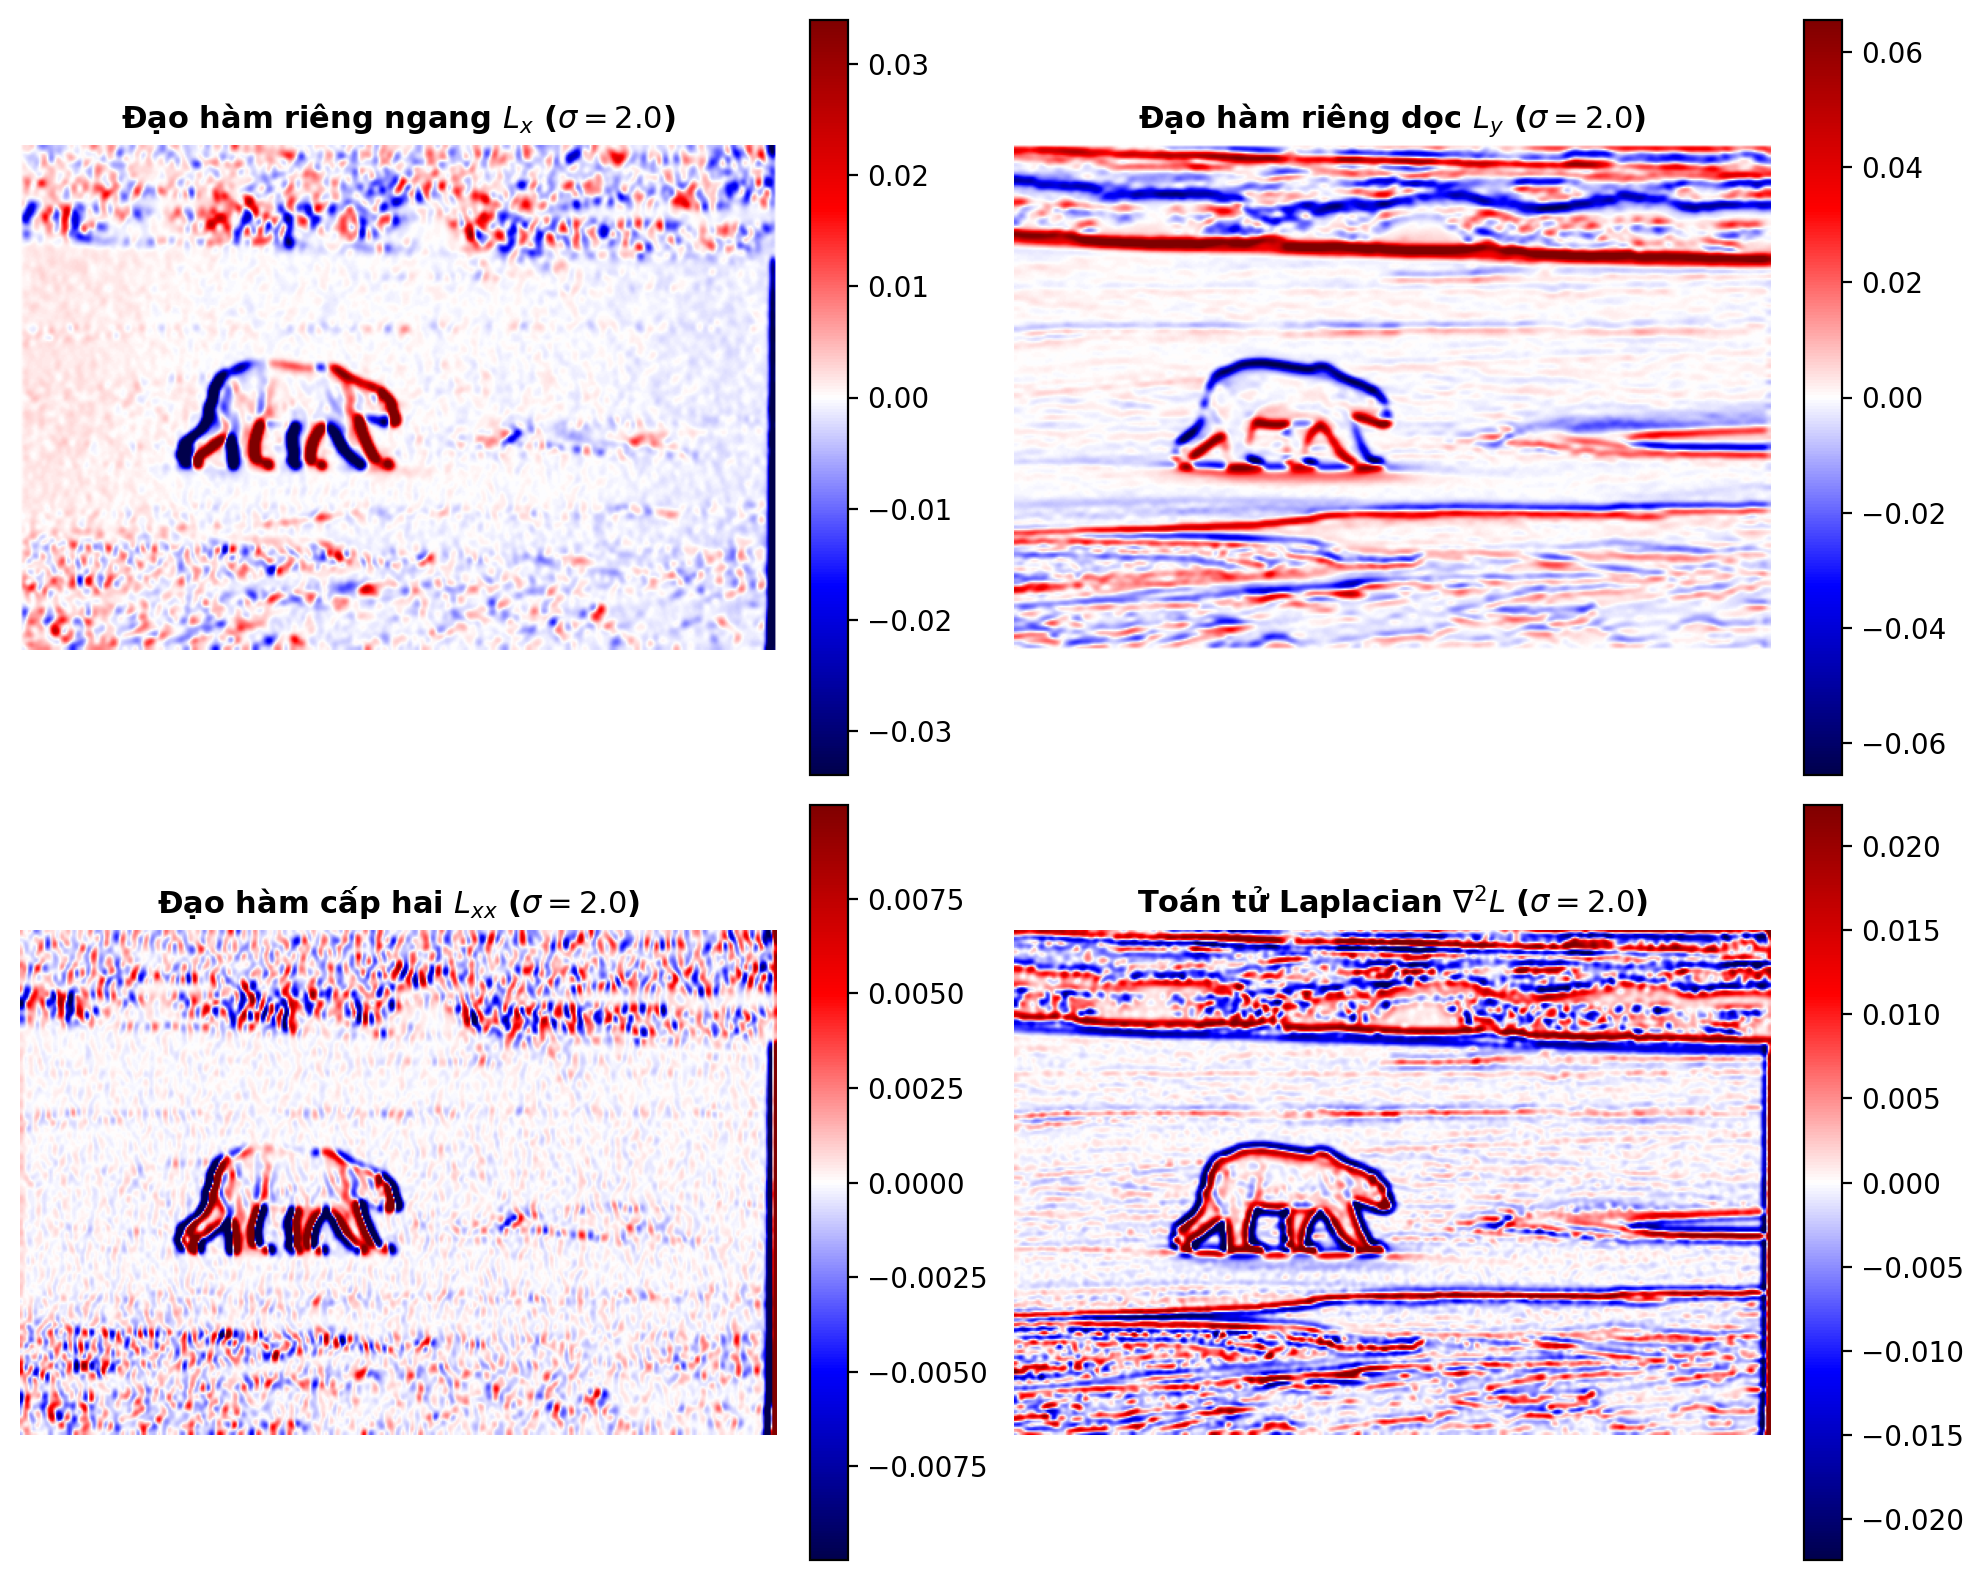
\includegraphics[width=0.48\textwidth]{figures/showcase_scientific_diverging_maps.png}
\caption{Ví dụ các bản đồ đạo hàm trên ảnh BSDS500 tại $\sigma=2$: $L_x$, $L_y$, $L_{xx}$ và $\nabla^2L$. Màu phân kỳ biểu diễn dấu và biên độ của đáp ứng.}
\label{fig:derivative_maps}
\end{figure}

\subsection{Thiết Kế và Cài Đặt 3 Bộ Dò Đặc Trưng Mức Cao}

\subsubsection{Bộ dò biên đa tỷ lệ Canny (Canny Edge Detector)}
Quy trình phát hiện biên Canny \cite{canny1986computational} được xây dựng độc lập gồm 3 công đoạn chính:
\begin{enumerate}
    \item \textbf{Làm mịn và Gradient đa tỷ lệ:} Sử dụng cặp đạo hàm $L_x, L_y$ tại tỷ lệ $\sigma$ xác định.
    \item \textbf{Triệt tiêu không cực đại (NMS):} Góc pháp tuyến $\theta = \operatorname{arctan2}(L_y, L_x)$ được lượng tử hóa thành bốn hướng không phân biệt chiều: $0^\circ$, $45^\circ$, $90^\circ$ và $135^\circ$. Một pixel được giữ nếu độ lớn gradient không nhỏ hơn hai điểm lân cận dọc theo hướng gradient.
    \item \textbf{Phân ngưỡng kép và loang liên thông BFS (hysteresis):} Điểm ảnh được chia thành biên mạnh, biên yếu và nền theo hai ngưỡng. BFS dùng hàng đợi thay cho đệ quy, tránh phụ thuộc vào giới hạn độ sâu đệ quy; từ mỗi điểm mạnh, thuật toán lan theo 8 lân cận để giữ các điểm yếu liên thông.
\end{enumerate}

\subsubsection{Bộ lọc mạch máu đa tỷ lệ Frangi (Frangi Vesselness Filter)}
Dựa trên phân tích hình học ma trận Hessian \cite{frangi1998multiscale}, ridge có một trị riêng nhỏ theo hướng dọc thân và một trị riêng lớn theo hướng ngang thân. Sau khi sắp theo độ lớn, ký hiệu $|\lambda_1|\leq|\lambda_2|$; dấu của $\lambda_2$ phân biệt ridge sáng và rãnh tối. Với ảnh DRIVE kênh Green, mạch máu là rãnh tối trên nền sáng nên phép dò giữ đáp ứng có $\lambda_2>0$.
Hệ thống cài đặt bộ lọc Frangi với chuẩn hóa tỷ lệ theo Lindeberg \cite{lindeberg1998feature} ($\gamma = 1.0$):
\begin{align}
\mathcal{R}_B &= \frac{|\lambda_1|}{|\lambda_2|} \quad \text{(Độ đo dạng đốm/blobness)} \\
\mathcal{S} &= \sqrt{\lambda_1^2 + \lambda_2^2} \quad \text{(Độ đo cấu trúc Frobenius)}
\end{align}
Hàm đáp ứng mạch máu tại tỷ lệ $\sigma$ được tính theo công thức:
\begin{equation}
V_0(x, y; \sigma) = \begin{cases}
    0 & \text{nếu } \lambda_2 \leq 0 \\
    \exp\left(-\frac{\mathcal{R}_B^2}{2\beta^2}\right) \left[ 1 - \exp\left(-\frac{\mathcal{S}^2}{2c^2}\right) \right] & \text{nếu } \lambda_2 > 0
\end{cases}
\end{equation}
với $\beta = 0.5$ và ngưỡng cấu trúc thích nghi $c = 0.5 \cdot \max_{(x,y)} \mathcal{S}(x, y; \sigma)$.
Bản đồ mạch máu hoàn chỉnh được tổng hợp thông qua nguyên lý chọn tỷ lệ cực đại xuyên suốt không gian scale:
\begin{equation}
V_{\text{final}}(x, y) = \max_{\sigma \in \Sigma} V_0(x, y; \sigma)
\end{equation}

\subsubsection{Bộ dò đốm đa tỷ lệ LoG (Laplacian of Gaussian Blob Detector)}
Đốm (Blob) là các cấu trúc lồi/lõm tròn đối xứng có mức xám tương phản cục bộ.
Hệ thống sử dụng toán tử Laplace chuẩn hóa tỷ lệ (Normalized Laplacian of Gaussian):
\begin{equation}
\nabla_{\text{norm}}^2 L(x, y; \sigma) = \sigma^2 |L_{xx}(x, y; \sigma) + L_{yy}(x, y; \sigma)|
\end{equation}
Nhân tử $\sigma^2$ hỗ trợ so sánh đáp ứng bậc hai giữa các tỷ lệ. Độ nhạy thực tế vẫn phụ thuộc hình dạng đối tượng, lưới tỷ lệ, tương phản và ngưỡng.
\begin{itemize}
    \item \textbf{Lưới tỷ lệ hình học:} Xây dựng không gian tỷ lệ 3D gồm tập hợp các tỷ lệ tăng theo cấp số nhân bước $k = \sqrt{2}$: $\Sigma = \{\sigma_0, \sqrt{2}\sigma_0, 2\sigma_0, 2\sqrt{2}\sigma_0, \dots, 8.0\}$.
    \item \textbf{Triệt tiêu không cực đại 3D (3D Non-Maximum Suppression):} Một điểm $(y, x, \sigma)$ được xác định là tâm đốm nếu đáp ứng $\nabla_{\text{norm}}^2 L(y, x; \sigma)$ lớn hơn ngưỡng cường độ tối thiểu $T_{\text{blob}}$ và là cực đại tuyệt đối so với toàn bộ $26$ lân cận trong khối cầu $3 \times 3 \times 3$ (8 lân cận không gian cùng lớp scale và $9 \times 2 = 18$ lân cận tại hai lớp scale liền kề $\sigma_{i-1}, \sigma_{i+1}$).
    \item \textbf{Ước lượng kích thước:} Repo dùng quy ước $R\approx\sqrt2\sigma$ trong 2D để biểu diễn bán kính từ tỷ lệ đặc trưng; quan hệ này phụ thuộc mô hình đối tượng, không phải bán kính thật chính xác của mọi tế bào.
\end{itemize}

\subsection{Thiết kế hiệu chuẩn bằng ảnh giải tích}
Một bộ lọc có đầu ra trông hợp lý vẫn có thể sai dấu, sai hệ số tỷ lệ hoặc sai thứ tự trục. Vì vậy, trước khi đọc kết quả trên ảnh tự nhiên, cần kiểm tra bằng ảnh có đạo hàm biết trước. Phần này mô tả các phép kiểm soát phù hợp với quy ước của dự án; không thay thế các phép đo thực tế bằng giá trị kỳ vọng lý thuyết.

\subsubsection{Ảnh hằng và kiểm tra thành phần DC}
Với $I(x,y)=c$, Gaussian phải trả gần $c$ và mọi đạo hàm bậc dương phải gần 0 trong vùng lõi. Nếu kernel đạo hàm có tổng $\eta\neq0$, một nền hằng tạo sai lệch xấp xỉ $c\eta$. Khi $c$ lớn, sai lệch này có thể làm bản đồ bậc hai xuất hiện nền khác 0 dù ảnh không có cấu trúc.

Kiểm tra ảnh hằng cũng giúp phát hiện một lỗi trao đổi dữ liệu: chuyển bản đồ có dấu sang uint8 có thể tạo clipping hoặc cuộn giá trị, làm thống kê sai lệch dù công thức lọc đúng. Cần kiểm tra dtype và miền giá trị trước khi quy sai số cho thuật toán.

\subsubsection{Ảnh dốc và kiểm tra dấu}
Với $I(x,y)=x$, kỳ vọng trong mô hình liên tục là $L_x=1$, $L_y=0$ và các đạo hàm bậc hai bằng 0. Nếu $L_x$ gần $-1$, một khả năng là tích chập đã được thực hiện như tương quan với kernel bậc lẻ. Nếu $L_x$ gần $\sigma$, cần kiểm tra chuẩn hóa theo tỷ lệ đã được áp dụng ở nguồn nào.

Ảnh dốc không thích hợp để nghiệm thu sai số tương đối cho những toán tử có đáp ứng tham chiếu bằng 0: mẫu số chuẩn hóa gần 0 làm tỷ số rất nhạy. Do đó dự án dùng thêm ảnh tự nhiên bất đối xứng cho phép so khớp đầy đủ.

\subsubsection{Ảnh parabol và kiểm tra bậc hai}
Với $I=x^2/2$, kỳ vọng $L_{xx}=1$, $L_{yy}=L_{xy}=0$ và $\nabla^2L=1$. Phép đo trên nhiều $\sigma$ phân biệt đạo hàm thô với bản đồ đã nhân $\sigma^2$. Trên ảnh hữu hạn, đo ở giữa ảnh để tránh ảnh hưởng của kiểu đệm.

Đặt gốc tọa độ ở tâm ảnh giúp giảm biên độ của đa thức so với dùng tọa độ luôn dương. Điều này giảm mất mát chữ số có nghĩa khi dữ liệu được ghi float32 rồi đưa qua các phép trừ trong tính vi phân. Tuy vậy, đây là cách giảm điều kiện số học bất lợi, không loại bỏ hoàn toàn sai số làm tròn.

\subsubsection{Ảnh yên ngựa và kiểm tra trị riêng}
Xét $I=x^2/2-y^2$. Hessian là $\operatorname{diag}(1,-2)$, nên thứ tự đại số cho $(1,-2)$, còn thứ tự theo độ lớn sẽ đặt trị riêng $-2$ trước trị riêng $1$. Ví dụ này phân biệt ba thao tác thường bị nhầm: sắp thứ tự đại số, sắp theo độ lớn nhưng giữ dấu, và thay trị riêng bằng trị tuyệt đối.

Để kiểm tra phần tử ngoài đường chéo, thêm thành phần $bxy$. Khi đó $L_{xy}=b$ và hai vector riêng thay đổi hướng. Chỉ dùng ảnh có Hessian chéo sẽ không phát hiện được việc cài đặt $L_{xy}$ sai.

\subsubsection{Ảnh xung và kiểm tra kernel}
Với ảnh xung Dirac ở giữa, đáp ứng của toán tử tuyến tính chính là kernel hiệu dụng sau rời rạc hóa và cắt cụt. Từ đáp ứng có thể đọc đối xứng chẵn/lẻ, tổng trọng số, độ rộng hỗ trợ và dấu đạo hàm. Nếu hai kernel cùng dạng nhưng khác một hệ số, tương quan đầu ra có thể rất cao; kiểm tra moment và biên độ giúp nhận biết sai khác này.

Ảnh xung nhỏ chỉ thích hợp với các $\sigma$ có vùng hỗ trợ nằm gọn trong ảnh. Không tăng $\sigma$ tới mức kernel gần bằng kích thước ảnh rồi coi đó là phép đo kernel trong miền vô hạn.

\subsection{Moment rời rạc và hệ số của bộ lọc}
Với tích chập một chiều $D_mI[x]=\sum_n h_m[n]I[x-n]$, khai triển
\begin{equation}
I[x-n]=\sum_{p=0}^{P}\frac{(-n)^p}{p!}I^{(p)}[x]+\text{phần dư}.
\end{equation}
Để chọn đạo hàm bậc $m$ trên các đa thức bậc không vượt quá $m$, các moment cần thỏa
\begin{equation}
\sum_n n^p h_m[n]=(-1)^m m!\,\delta_{pm},
\quad p=0,\ldots,m.
\label{eq:discrete_moments_detail}
\end{equation}
Với $m=1$, tổng kernel bằng 0 và moment bậc nhất bằng $-1$ theo quy ước tích chập này. Với $m=2$, tổng bằng 0, moment bậc nhất bằng 0 và moment bậc hai bằng 2. Kernel chẵn/lẻ giúp thỏa một số điều kiện tự động trong số học chính xác, nhưng cắt cụt và dấu chấm động vẫn cần được kiểm tra.

Các điều kiện trên xác định những đáp ứng đa thức cục bộ cần bảo toàn, không khẳng định kernel lấy mẫu và kernel hiệu chỉnh moment có cùng hệ số ở mọi vị trí. Đây là lý do sai khác có hệ thống giữa hai bộ cài đặt có thể còn tồn tại khi cùng dùng công thức Gaussian liên tục.

\subsection{Tích chập và tương quan}
Hai phép toán có dạng gần giống nhau:
\begin{equation}
(I*h)[x]=\sum_n h[n]I[x-n],\qquad
(I\star h)[x]=\sum_n h[n]I[x+n].
\end{equation}
Nếu $h$ chẵn như Gaussian hoặc đạo hàm bậc hai, đảo kernel không làm đổi dấu. Nếu $h$ lẻ như đạo hàm bậc nhất, đảo kernel đổi dấu đáp ứng. Vì vậy chỉ đối chiếu Gaussian smoothing là chưa đủ để xác nhận phép chập đúng.

Với đạo hàm hỗn hợp $L_{xy}$, hai phép đạo hàm lẻ cùng đổi dấu có thể triệt tiêu nhau. Một bộ cài đặt sai dấu ở cả hai trục có thể vẫn cho $L_{xy}$ gần đúng trong khi $L_x,L_y$ sai dấu. Bộ kiểm tra cần bao gồm cả đạo hàm đơn trục và hỗn hợp.

\subsection{Đệm biên và vùng lõi hợp lệ}
Với tín hiệu có các giá trị $a,b,c,d$, hai quy tắc phản xạ cần phân biệt là
\begin{align*}
\text{lặp pixel biên: }&\cdots c\,b\,a\mid a\,b\,c\,d\mid d\,c\,b\cdots,\\
\text{không lặp biên: }&\cdots d\,c\,b\mid a\,b\,c\,d\mid c\,b\,a\cdots.
\end{align*}
Tên reflect và mirror phụ thuộc API: NumPy pad reflect tương ứng quy tắc không lặp pixel biên, trong khi SciPy dùng tên mirror cho quy tắc đó. Không nên kết luận hai thư viện dùng cùng điều kiện biên chỉ vì cùng thấy từ reflect.

Nếu kernel có bán kính $r$, pixel cách mép không quá $r$ có thể chịu ảnh hưởng từ phần đệm. Với tensor gồm hai giai đoạn lọc, hỗ trợ hiệu dụng cộng từ cả hai bước. Đối chiếu trong vùng lõi giúp tập trung vào toán tử; đánh giá riêng vùng biên vẫn cần thiết nếu mục tiêu là ứng dụng trên toàn ảnh.

\subsection{Hợp đồng dữ liệu giữa các mô-đun}
Một bản đồ không chỉ được nhận diện bởi tên toán tử. Bộ siêu dữ liệu tối thiểu gồm nguồn, ảnh, $\sigma$, bậc đạo hàm, chuẩn hóa, thứ tự trị riêng, đơn vị không gian, dtype và kiểu biên. Hai TIFF cùng tên nhưng thuộc hai phiên bản config khác nhau chưa phải một cặp đối chiếu hợp lệ.

Nhân tính toán làm việc trên float64, còn trao đổi giữa hai môi trường dùng TIFF float32 không nén. Sai số sau xuất TIFF vì thế bao gồm cả làm tròn về float32. Không đem một kết quả float64 trong bộ nhớ so với một ảnh PNG 8-bit đã giãn tương phản rồi gọi đó là sai số thuật toán.

\begin{figure*}[t]
\centering
\begin{minipage}{0.94\textwidth}
\begin{algorithmic}[1]
\STATE Đọc config và dừng nếu còn tham số null.
\STATE Đọc cùng ảnh xám uint8, chuyển bản sao làm việc sang float64.
\FOR{mỗi $\sigma$ trong cấu hình}
\STATE Sinh $g_0,g_1,g_2$ với bán kính theo từng bậc.
\STATE Tính $L,L_x,L_y,L_{xx},L_{xy},L_{yy}$ bằng chập tách trục.
\STATE Tạo gradient, Laplacian, Hessian và tensor theo nhu cầu.
\STATE Giữ bản đồ thô để đối chiếu; tạo bản chuẩn hóa riêng cho bộ dò.
\STATE Xuất TIFF float32, tên file và metadata nhất quán.
\ENDFOR
\end{algorithmic}
\end{minipage}
\caption{Mã giả luồng tính toán và kiểm soát quy ước dữ liệu}
\end{figure*}

\subsection{Mã giả phép đối chiếu và kiểm soát sai sót}
\begin{figure*}[t]
\centering
\begin{minipage}{0.94\textwidth}
\begin{algorithmic}[1]
\FOR{mỗi cặp ảnh, toán tử và tỷ lệ được yêu cầu}
\IF{thiếu một TIFF}
\STATE Ghi trạng thái thiếu dữ liệu; không thay bằng ảnh 0.
\ELSE
\STATE Kiểm tra kích thước, float32 và giá trị hữu hạn.
\STATE Xác định vùng crop từ config và hỗ trợ toán tử.
\STATE Tính max error, MAE, RMSE, relative max error và Pearson.
\STATE Xếp loại theo tiêu chí đã công bố; ghi cả trường hợp không đạt.
\ENDIF
\ENDFOR
\STATE Tổng hợp số cặp đã đo, thiếu dữ liệu và số cặp theo từng trạng thái.
\end{algorithmic}
\end{minipage}
\caption{Mã giả đối chiếu số học; số lượng cặp hợp lệ là một phần của kết quả}
\end{figure*}
Việc kiểm tra đủ số cặp quan trọng ngang việc báo cáo trung bình. Nếu các cặp khó hoặc file thiếu bị bỏ qua âm thầm, điểm trung bình có thể tăng mà không phản ánh chất lượng tốt hơn. Bản ghi CSV cần cho phép truy ngược từ một dòng tổng hợp về TIFF và cấu hình cụ thể.

\subsection{Thiết kế kiểm tra độ nhạy có kiểm soát}
Ngoài benchmark hiện có, có thể thiết kế một chuỗi thí nghiệm thay đổi từng yếu tố: giữ ảnh và ngưỡng để khảo sát $\sigma$; giữ $\sigma$ để khảo sát ngưỡng; giữ ảnh sạch làm tham chiếu rồi thêm các mức nhiễu đã biết. Các thí nghiệm này là hướng mở rộng cần chạy và ghi kết quả, chưa phải các kết quả đã đo trong báo cáo.

Với biến đổi tương phản tuyến tính $I'=aI+b$, đạo hàm bậc dương trong vùng lõi đáp ứng $D(I')=aD(I)$; Hessian cũng nhân $a$, còn Structure Tensor nhân $a^2$. Kiểm tra quan hệ này có thể phát hiện việc đổi miền cường độ hoặc chuẩn hóa hiển thị bị đưa nhầm vào nhân tính toán. Khi $a<0$, dấu đạo hàm và cực tính ridge/blob đảo; độ lớn gradient và tensor không đổi dấu.

Với nhiễu độc lập có phương sai $\sigma_n^2$, phương sai đầu ra của một bộ lọc tuyến tính rời rạc $h$ là $\sigma_n^2\sum h^2$ trong vùng không biên. Quan hệ này giải thích vì sao kernel và mức làm mịn ảnh hưởng độ nhạy với nhiễu. Nó không thay cho việc đo trên ảnh thực với nhiễu tương quan hoặc nhiễu phụ thuộc cường độ.


\subsection{Chiến Lược Tối Ưu Hóa và Phân Tích Độ Phức Tạp Thuật Toán}
\subsubsection{Vector hóa toàn phần bằng NumPy (Array Broadcasting)}
Các phép tính theo pixel được biểu diễn dưới dạng phép toán mảng NumPy thay cho vòng lặp Python lồng nhau. NumPy gọi các thư viện số học native của môi trường cài đặt; tốc độ thực tế phụ thuộc vào phiên bản NumPy, thư viện BLAS và phần cứng, nên báo cáo không suy ra hiệu năng SIMD cụ thể nếu chưa đo.

\subsubsection{Quản lý độ chính xác số học và Bộ nhớ}
Quá trình tính toán trung gian được duy trì ở kiểu số thực dấu chấm động độ chính xác kép \texttt{float64} (64-bit). Điều này ngăn ngừa sai số tích lũy từ các phép nhân dồn và phép trừ ma trận có độ lệch giá trị nhỏ. Chỉ tại bước cuối cùng khi xuất file ảnh lưu trữ đĩa (TIFF 32-bit), dữ liệu mới được ép kiểu an toàn sang \texttt{float32}.

\subsubsection{Bảng tổng hợp độ phức tạp thuật toán}
\begin{table}[htbp]
\caption{Độ phức tạp thời gian và không gian của các mô-đun lõi}
\centering
\begin{tabular}{lcc}
\toprule
\textbf{Mô-đun / Thuật toán} & \textbf{Độ phức tạp thời gian} & \textbf{Độ phức tạp bộ nhớ} \\
\midrule
Gaussian Smoothing 2D tách trục & $\mathcal{O}(2K \cdot HW)$ & $\mathcal{O}(HW)$ \\
Gradient $(L_x,L_y)$ & $\mathcal{O}(4K \cdot HW)$ & $\mathcal{O}(HW)$ \\
Ma trận Hessian \& Trị riêng & $\mathcal{O}(6K \cdot HW)$ & $\mathcal{O}(HW)$ \\
Structure Tensor $(\sigma_d, \sigma_i)$ & $\mathcal{O}((4K_d + 6K_i) \cdot HW)$ & $\mathcal{O}(HW)$ \\
Canny NMS \& Hysteresis BFS & $\mathcal{O}(HW)$ & $\mathcal{O}(HW)$ \\
Frangi Filter ($|\Sigma|$ tỷ lệ) & $\mathcal{O}(|\Sigma| \cdot 6K \cdot HW)$ & $\mathcal{O}(HW)$ \\
LoG Extrema 3D ($|\Sigma|$ tỷ lệ) & $\mathcal{O}(|\Sigma| \cdot HW)$ & $\mathcal{O}(|\Sigma| \cdot HW)$ \\
\bottomrule
\end{tabular}
\label{tab:complexity}
\end{table}

\section{Chương 5: Thực Nghiệm, Đánh Giá Định Lượng và Phân Tích}
\subsection{Thiết kế đánh giá}
Đánh giá được chia thành hai câu hỏi. Tầng 1 đo độ tương đồng số học giữa các bản đồ liên tục của Python Core và FeatureJ trên năm ảnh đại diện; vùng biên bị crop theo bán kính kernel trước khi tính sai số tương đối và Pearson $r$. Bản đồ được xếp \texttt{STRICT} nếu $\mathrm{rel\_err}<10^{-4}$ và $r>0.9999$, \texttt{RELAXED} nếu $\mathrm{rel\_err}<10^{-2}$ và $r>0.9999$.

Tầng 2 đo chất lượng phát hiện so với nhãn tham chiếu: BSDS500 dùng dung sai biên $\pm2$ pixel; DRIVE tính F1/IoU bên trong FOV đã xói mòn với bán kính phụ thuộc $\sigma$; Blobs ghép tâm trong 2 pixel và bán kính trong sai số 20\%. Ngưỡng Canny được chọn từ lưới trên cùng 10 ảnh BSDS500; tại $\sigma=2$, cặp đã chọn là $p_{\mathrm{low}}=67$ và $p_{\mathrm{high}}=91$. Việc chọn và đánh giá trên cùng tập có thể làm F1 lạc quan hơn. Điểm F1 trong bảng tổng hợp là trung bình theo ảnh, trừ khi ghi rõ micro-average.

\subsection{Định nghĩa các thước đo và cách tổng hợp}
\label{sec:metrics}
\subsubsection{Sai số trên bản đồ liên tục}
Gọi $P_i$ và $F_i$ là giá trị Python và FeatureJ sau khi đã cắt vùng biên, với $N$ pixel còn lại. Các thước đo có trong CSV gồm
\begin{align}
E_{\max}&=\max_i|P_i-F_i|,\\
\mathrm{MAE}&=\frac1N\sum_i|P_i-F_i|,\\
\mathrm{RMSE}&=\sqrt{\frac1N\sum_i(P_i-F_i)^2}.
\end{align}
Trong verify\_tier1.py của repo, sai số tương đối được định nghĩa cụ thể là
\begin{equation}
E_{\mathrm{rel}}=\frac{E_{\max}}{\max_i|F_i|+10^{-12}}.
\label{eq:relmax}
\end{equation}
Đây là sai số cực đại chuẩn hóa theo đỉnh của bản đồ tham chiếu, không phải sai số tương đối theo chuẩn $L_2$. Định nghĩa phải đi kèm con số phần trăm vì các cách chuẩn hóa khác nhau có thể cho giá trị rất khác.

Hệ số Pearson đo sự đồng biến tuyến tính:
\begin{equation}
r=\frac{\sum_i(P_i-\overline P)(F_i-\overline F)}
{\sqrt{\sum_i(P_i-\overline P)^2\sum_i(F_i-\overline F)^2}}.
\end{equation}
Nếu $P=aF+b$ với $a>0$ và $F$ không hằng, Pearson bằng 1 dù có sai số biên độ hoặc độ lệch nền. Vì thế phải đọc Pearson cùng MAE, RMSE và $E_{\mathrm{rel}}$. Với ảnh gần hằng, phương sai rất nhỏ làm Pearson kém ổn định; trường hợp này cần xử lý riêng theo evaluator thay vì tự gán một giá trị tương quan có ý nghĩa.

PSNR cho ảnh Gaussian trong miền cường độ 8-bit được tính bằng $20\log_{10}(255/\mathrm{RMSE})$. Repo không dùng cách diễn giải này cho mọi bản đồ có dấu: đạo hàm và trị riêng không còn có cùng miền vật lý $[0,255]$. Chọn một đỉnh cố định không phù hợp có thể làm PSNR lớn nhưng khó diễn giải.

\subsubsection{Precision, recall, F1 và IoU}
Với phát hiện nhị phân, gọi TP, FP và FN lần lượt là số dương tính đúng, dương tính sai và âm tính sai. Ta có
\begin{align}
\mathrm{Precision}&=\frac{\mathrm{TP}}{\mathrm{TP}+\mathrm{FP}},\\
\mathrm{Recall}&=\frac{\mathrm{TP}}{\mathrm{TP}+\mathrm{FN}},\\
F_1&=\frac{2\mathrm{TP}}{2\mathrm{TP}+\mathrm{FP}+\mathrm{FN}},\\
\mathrm{IoU}&=\frac{\mathrm{TP}}{\mathrm{TP}+\mathrm{FP}+\mathrm{FN}}.
\end{align}
Trong triển khai cần xử lý mẫu số bằng 0. Precision cao phản ánh ít phát hiện nhầm, recall cao phản ánh ít bỏ sót. F1 cân bằng hai đại lượng nhưng không thể hiện đầy đủ vị trí lỗi, độ dày mạch hoặc chất lượng định vị tâm.

Với cùng một ma trận nhầm lẫn, $F_1=2\,\mathrm{IoU}/(1+\mathrm{IoU})$. Tuy nhiên, không nên lấy IoU trung bình của nhiều ảnh rồi biến đổi để khẳng định đó là F1 trung bình, vì phép biến đổi phi tuyến không giao hoán với phép lấy trung bình.

\subsubsection{Macro và micro}
Macro-$F_1$ là trung bình $F_{1,j}$ theo ảnh, còn micro-$F_1$ gộp TP/FP/FN trước khi tính:
\begin{equation}
\begin{aligned}
F_{1,\mathrm{macro}} &= \frac{1}{M}\sum_{j=1}^{M}F_{1,j}, \\
F_{1,\mathrm{micro}} &=
\frac{2\sum_j\mathrm{TP}_j}
{2\sum_j\mathrm{TP}_j+\sum_j\mathrm{FP}_j+\sum_j\mathrm{FN}_j}.
\end{aligned}
\end{equation}
Bốn ảnh Blob tổng hợp có ít đối tượng và đạt điểm cao, trong khi ảnh sinh học có hàng trăm đối tượng. Macro cho mỗi ảnh trọng số bằng nhau; micro bị ảnh có nhiều đối tượng chi phối. Cần ghi rõ cách tổng hợp, không dùng một giá trị macro cao để bỏ qua lỗi trên ảnh sinh học.

\subsection{Giao thức đánh giá riêng cho ba bài toán}
\subsubsection{Đường biên BSDS500}
Đường biên chỉ dày một vài pixel nên một dịch chuyển nhỏ có thể làm giảm điểm nếu yêu cầu trùng pixel tuyệt đối. Repo dùng phần tử cấu trúc là đĩa Euclidean bán kính 2 pixel (13 pixel trong ô 5$\times$5), không gồm các góc, và xử lý nhiều nhãn annotator. Ảnh không có pixel sau NMS vẫn nằm trong mẫu số với F1 bằng 0. Báo cáo mô tả đây là giao thức evaluator của dự án, không mặc nhiên đồng nhất với toàn bộ benchmark BSDS500 chính thức hoặc các điểm ODS/OIS trong tài liệu khác.

Phân vị $p$ không phải một ngưỡng cường độ cố định: giá trị số tương ứng phụ thuộc phân bố đáp ứng của ảnh và tập pixel được dùng để tính phân vị. Khi so sánh Python với Fiji cần dùng cùng thuật toán tính phân vị và cùng bước hậu xử lý. Chọn riêng ngưỡng tối ưu cho mỗi nhánh sẽ đồng thời thay đổi toán tử và cách ra quyết định, làm kết luận về độ tương đương khó xác định.

\subsubsection{Vùng mạch máu DRIVE}
Vùng đánh giá phải nằm trong trường nhìn hợp lệ. Viền giữa đĩa võng mạc và nền đen có tương phản mạnh, dễ tạo đáp ứng Hessian lớn dù không phải mạch. Repo áp dụng FOV xói mòn phụ thuộc tỷ lệ để giảm ảnh hưởng này. Cần ghi rõ mặt nạ dùng trong điểm số: một phương pháp được chấm trên vùng nhỏ hơn không thể so sánh trực tiếp với phương pháp chấm trên toàn FOV.

F1/IoU ở đây phản ánh phân đoạn vùng mạch, không phải độ đúng của một bộ đường tâm ridge đã skeleton hóa. Mạch nhỏ, nhánh giao nhau và các đoạn tương phản yếu là các trường hợp cần đọc trên hình ngoài điểm số.

\subsubsection{Danh sách đối tượng Blob}
Mỗi dự đoán gồm tọa độ tâm và kích thước. Repo ghép tâm với dung sai 2 pixel, đồng thời yêu cầu sai số bán kính tương đối không quá 20\%. Mỗi nhãn chỉ được ghép một lần; các dự đoán thừa xung quanh cùng một tế bào không được tính là nhiều TP. Ngoài điểm F1, cần xem độ nhạy của phép ghép đối với các nhãn tâm gần nhau và kích thước do người gán nhãn xác định.

Theo kết quả canonical, blob\_05 có 276 đối tượng nhãn; Python chính thức ở lưới 8 mức phát hiện 329 và ghép đúng 140, nên FP=189, FN=136 và $F_1=280/(280+189+136)\approx0.4628$. Fiji fair ở lưới 7 mức cũng có 329 phát hiện nhưng ghép đúng 139, cho $F_1\approx0.4595$. Hai lưới scale khác nhau. Hàng Python 7 mức, 326 phát hiện và $F_1=0.4651$ nằm trong CSV so sánh chung nhưng không phải kết quả Python chính thức. Ví dụ này cho thấy recall $140/276$ không phải F1; chỉ nêu tỷ lệ bắt trúng sẽ bỏ qua phát hiện thừa.

\subsection{Thiết kế tái lập và trạng thái minh chứng}
Các bảng định lượng trong báo cáo được tổng hợp từ CSV của nhóm trong repo, không được trình bày như kết quả vừa chạy mới trên máy biên tập. Phương án thực hành bổ sung là chạy ba ảnh mẫu trên Fiji và nhân Python, lưu vào thư mục riêng và lập CSV mới. Lần chạy mẫu mới đã có đủ 72 TIFF mỗi nhánh và CSV đối chiếu; các kết quả này được trình bày ở mục tái chạy mẫu. Chúng không thay thế bảng F1 tổng hợp của nhóm.

Khi thực hiện lần chạy bổ sung, cần lưu tên ảnh, mã phiên bản repo, config.yaml, phiên bản phần mềm và nguồn của từng TIFF. Nếu có sai khác so với bảng nhóm, kiểm tra cấu hình và nguồn file trước khi thay đổi nhận định. Một tập ba ảnh chỉ xác nhận thao tác và hành vi trên mẫu, không đủ để ước lượng lại F1 trung bình của tập 25 ảnh.


\subsection{Kết quả thẩm định Tầng 1 (So khớp Python Core với FeatureJ / Fiji)}
\begin{table*}[t]
\caption{Kết quả đối chuẩn định lượng trên 220 bản đồ liên tục}
\centering
\resizebox{\textwidth}{!}{\begin{tabular}{lcccc}
\toprule
\textbf{Toán tử} & \textbf{Sai số TB} & \textbf{Sai số tương đối} & \textbf{Pearson $r$ (Min)} & \textbf{Pearson $r$ (TB)} \\
\midrule
Gauss & 3.98e-07 & 7.32e-08 & 1.00000000 & 1.00000000 \\
$L_x$ & 2.74e-04 & 5.01e-04 & 1.00000000 & 1.00000000 \\
$L_y$ & 3.39e-04 & 5.01e-04 & 1.00000000 & 1.00000000 \\
Grad & 4.91e-04 & 5.01e-04 & 1.00000000 & 1.00000000 \\
$L_{xx}$ & 5.79e-03 & 4.21e-03 & 0.99998026 & 0.99999453 \\
$L_{yy}$ & 5.80e-03 & 4.40e-03 & 0.99996770 & 0.99999324 \\
$L_{xy}$ & 8.56e-05 & 1.00e-03 & 1.00000000 & 1.00000000 \\
Laplacian & 1.15e-02 & 4.44e-03 & 0.99996553 & 0.99999157 \\
Hessian L1 & 6.15e-03 & 4.43e-03 & 0.99997419 & 0.99999379 \\
Hessian L2 & 5.43e-03 & 3.33e-03 & 0.99997964 & 0.99999493 \\
ST L1 & 6.18e-03 & 4.40e-04 & 1.00000000 & 1.00000000 \\
ST L2 & 1.89e-03 & 4.40e-04 & 1.00000000 & 1.00000000 \\
\bottomrule
\end{tabular}}
\end{table*}

\textbf{Diễn giải:} Có 35/220 bản đồ đạt \texttt{STRICT} (20 bản đồ Gauss và 15 bản đồ đạo hàm bậc nhất tại $\sigma=1$); 185/220 chưa đạt tiêu chí gốc và chỉ được xếp \texttt{RELAXED} theo ngưỡng nới lỏng mang tính tham khảo; ngưỡng này không thay thế tiêu chí nghiệm thu gốc. Pearson trung bình toàn hệ thống là $0.99999710$, thấp nhất $0.99996553$. Sai số tương đối của đạo hàm bậc hai xấp xỉ $0.3$--$0.4\%$. Tương quan cao cho thấy hình dạng đáp ứng gần nhau, nhưng không có nghĩa biên độ của mọi bản đồ trùng nhau.

\subsection{Kết quả thực nghiệm Tầng 2 (so khớp Ground Truth)}
Các số liệu dưới đây được đồng bộ với metric snapshot canonical của repo tại commit \texttt{58bdfd8} và các CSV trong \texttt{outputs/metrics/}. Snapshot \texttt{duc\_08\_11} là dữ liệu lịch sử trước khi sửa dung sai BSDS từ ô vuông 5$\times$5 sang đĩa Euclidean 13 pixel.
Tập đánh giá gồm 10 ảnh BSDS500, 10 ảnh DRIVE và 5 ảnh Blob (bốn ảnh tổng hợp cùng một ảnh tế bào sinh học). Kết quả nhánh Python:
\begin{itemize}
    \item \textbf{BSDS500 (Canny Edge):} Theo giao thức canonical trên 10 ảnh BSDS500 \cite{arbelaez2010contour,xlaRepository}, ở $\sigma=2.0$ đạt $F_1=0.477886$ với $p_{\text{low}}=67$, $p_{\text{high}}=91$ và dung sai đĩa Euclidean bán kính 2 px (13 pixel). Ngưỡng được chọn trên chính tập ảnh này, không phải ước lượng độc lập trên tập kiểm tra.
    \item \textbf{DRIVE (Frangi Vesselness):} Thử nghiệm trên 10 ảnh mạch máu võng mạc DRIVE \cite{staal2004ridge,xlaRepository} đạt macro-$F_1=0.680633$, $\text{IoU}=0.5184$ trong vùng FOV xói mòn thích ứng đa tỷ lệ với bán kính $r=\lceil4\sigma\rceil$.
    \item \textbf{Blobs (LoG Scale-Space):} Macro-$F_1$ canonical Python/Fiji trên năm ảnh là $0.893023/0.891901$ \cite{xlaRepository}. Với \texttt{blob\_05}, kết quả Python chính thức ở lưới 8 mức là 140 cặp ghép đúng trong 329 phát hiện ($F_1=0.4628$); Fiji fair ở lưới 7 mức là 139/329 ($F_1=0.4595$). Hai lưới khác nhau; nhãn tế bào do nhóm xây dựng, không phải nhãn chuyên gia của nhà cung cấp.
\end{itemize}

Bảng~\ref{tab:tier2_cross} dùng cấu hình chung để đối chiếu Python--Fiji. Với Blobs, cả hai nhánh dùng bảy mức $\sigma=\{1,1.4,2,2.8,4,5.7,8\}$. Kết quả Python chính thức ở lưới 8 mức được lấy riêng từ \texttt{tier2\_results.csv}; không trộn với bảng so sánh 7 mức \cite{xlaRepository}.
\begin{table}[htbp]
\caption{Đối chiếu F1 macro Python--Fiji theo cấu hình so sánh chung 7 mức cho Blobs}
\label{tab:tier2_cross}
\centering
\begin{tabular}{lrrrr}
\toprule
\textbf{Tác vụ} & \textbf{$N$} & \textbf{Python} & \textbf{Fiji} & \textbf{$\Delta F_1$} \\
\midrule
BSDS500 / Canny, $\sigma=2$ & 10 & 0.4779 & 0.4779 & $0.0000$ \\
DRIVE / Frangi & 10 & 0.6806 & 0.6816 & $+0.0010$ \\
Blobs / LoG (7 mức) & 5 & 0.8930 & 0.8919 & $-0.0011$ \\
\bottomrule
\end{tabular}
\end{table}
Với DRIVE, IoU trung bình lần lượt là $0.5184$ (Python) và $0.5195$ (Fiji). Micro-$F_1$ trong bảng được tính lại từ tổng GT, số phát hiện và số ghép đúng ở CSV so sánh chung theo công thức trong Mục~\ref{sec:metrics}. Macro Python--Fiji của Blobs dùng lưới chung 7 mức; kết quả Python chính thức cho \texttt{blob\_05} ở lưới 8 mức được nêu riêng, nên hai giá trị per-image không phải so sánh cùng lưới. Chênh lệch F1 không thay thế đánh giá với Ground Truth.

\subsection{Kiểm tra tham chiếu ngoài nhân tính toán}
Phép hình thái học và gán nhãn thành phần trong bộ đánh giá BSDS hiện dùng NumPy thuần. SciPy chỉ được phép trong kiểm thử và benchmark thời gian; OpenCV được dùng làm tham chiếu trực quan bổ sung. Đầu ra Canny phụ thuộc vào kernel gradient, NMS và ngưỡng. Vì vậy, khác biệt hình ảnh giữa các thư viện không được diễn giải thành xếp hạng chất lượng nếu chưa cố định cùng dữ liệu, ngưỡng và tiêu chí chấm. Nhân toán học trong \texttt{src/core/} vẫn được triển khai bằng NumPy.
\begin{figure*}[t]
\centering
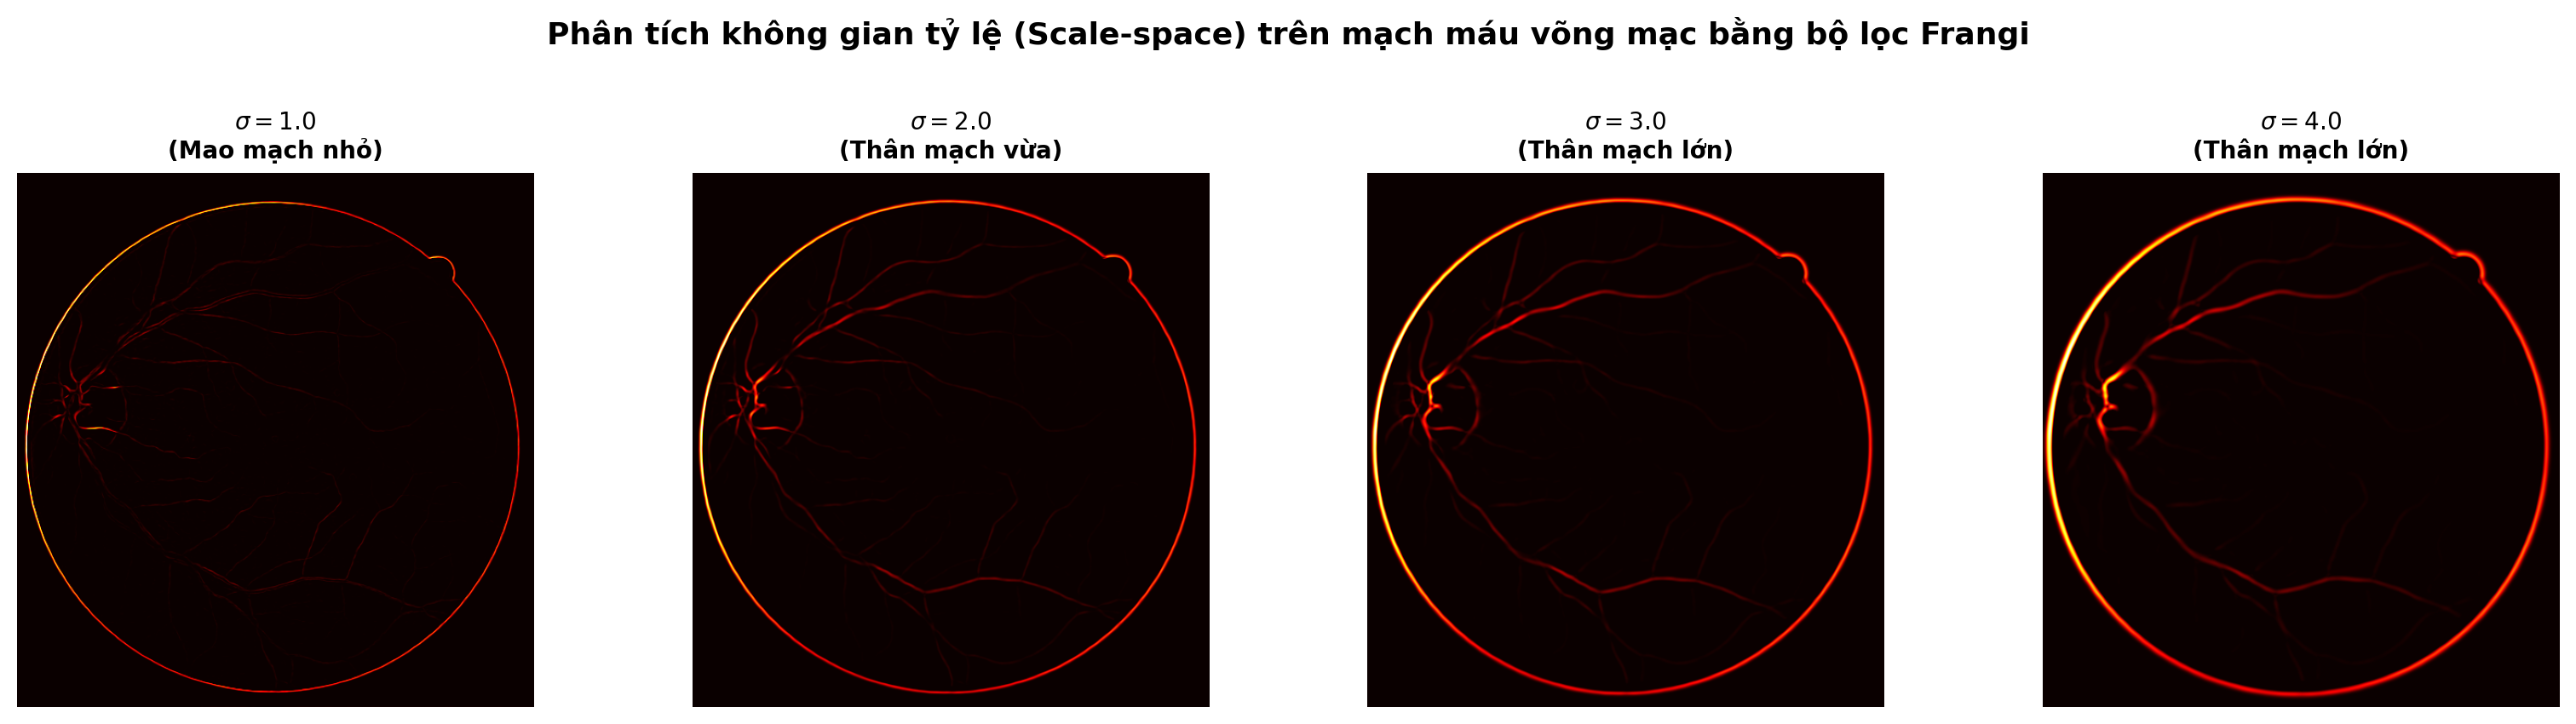
\includegraphics[width=0.92\textwidth]{figures/showcase_multiscale_frangi.png}
\caption{Đáp ứng Frangi trên ảnh DRIVE ở các tỷ lệ $\sigma\in\{1,2,3,4\}$. Phản ứng mạnh ở viền trường nhìn cho thấy vì sao benchmark loại vùng biên bằng mặt nạ FOV xói mòn trước khi tính điểm.}
\label{fig:multiscale_frangi}
\end{figure*}

\subsection{Phân Tích Chuyên Sâu Từng Bài Toán Thực Nghiệm}

\subsubsection{Bài toán dò biên BSDS500 (Canny)}
Đánh giá trên BSDS500 \cite{arbelaez2010contour} dùng đĩa Euclidean bán kính 2 pixel để ghép biên với nhãn đa annotator; các góc của ô vuông 5$\times$5 nằm ngoài dung sai. Trong lưới đã khảo sát, cấu hình $\sigma=2$, $p_{\mathrm{low}}=67$, $p_{\mathrm{high}}=91$ đạt F1 trung bình $0.477886$. Ngưỡng được chọn trên cùng tập ảnh dùng để báo cáo điểm, nên kết quả cần được xem là thực nghiệm thăm dò.

\begin{figure}[htbp]
\centering
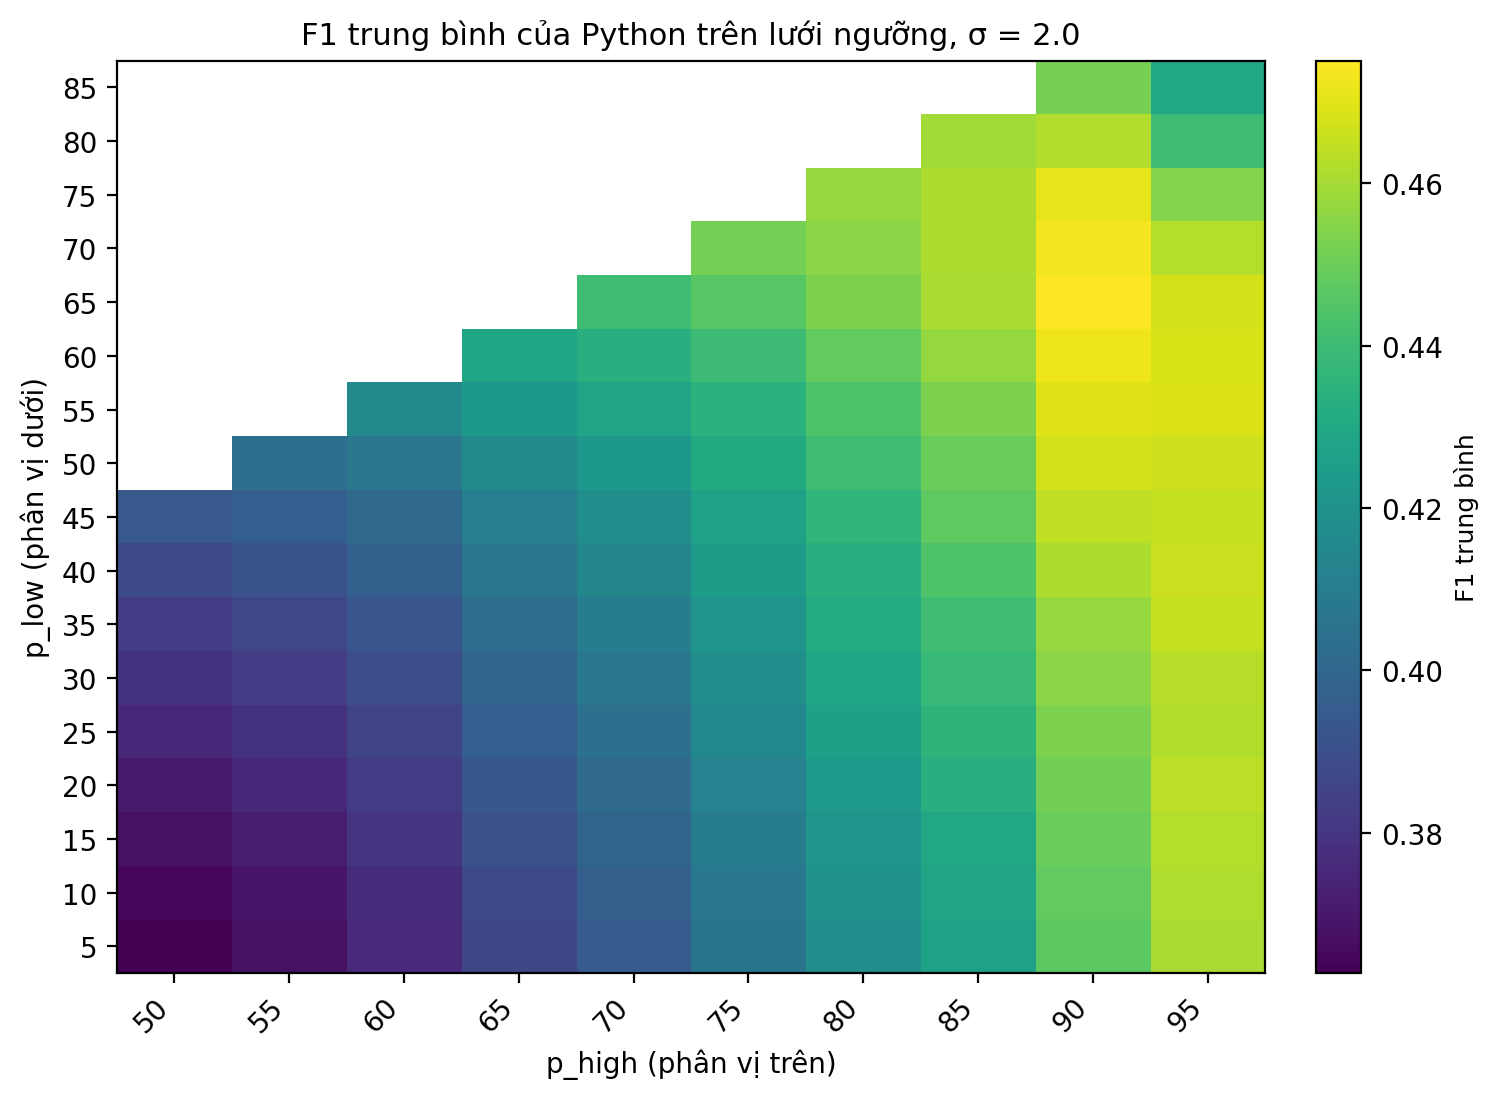
\includegraphics[width=0.48\textwidth]{figures/tier2_bsds_f1_heatmap.png}
\caption{Độ nhạy F1 trung bình trên BSDS500 theo hai phân vị ngưỡng tại $\sigma=2$. Cặp $p_{\mathrm{low}}=67$, $p_{\mathrm{high}}=91$ được cố định khi đối chiếu Python--Fiji ở tỷ lệ này.}
\label{fig:bsds_thresholds}
\end{figure}

\subsubsection{Bài toán dò mạch máu võng mạc DRIVE (Frangi)}
Trên 10 ảnh mạch máu đáy mắt DRIVE \cite{staal2004ridge}, pipeline đạt $F_1=0.6806$ và $\text{IoU}=0.5184$. Bước đánh giá áp dụng mặt nạ FOV xói mòn thích ứng đa tỷ lệ:
\begin{equation}
\mathcal{M}_{\text{FOV}}^{(\sigma)} = \mathcal{M}_{\text{FOV}} \ominus \mathcal{B}_{r(\sigma)}, \quad r(\sigma) = \lceil 4.0\sigma \rceil
\end{equation}
Mặt nạ xói mòn giảm ảnh hưởng của phản ứng giả gần đường viền nhãn cầu; phần đánh giá DRIVE chỉ tính trên vùng FOV còn lại.


\subsubsection{Bài toán dò đốm tế bào đa tỷ lệ (Blob LoG)}
Trên bốn ảnh tổng hợp \texttt{blob\_01}--\texttt{blob\_04}, phép dò đạt $F_1=1.000$ theo tiêu chí ghép của repo. Với \texttt{blob\_05}, kết quả Python chính thức ở lưới 8 mức là $F_1=0.4628$; Fiji fair ở lưới 7 mức đạt $F_1=0.4595$. Python 7 mức $0.4651$ là hàng trong CSV so sánh chung, không phải kết quả Python chính thức. Khoảng cách giữa ảnh tổng hợp và ảnh sinh học cho thấy mô hình blob lý tưởng chưa bao quát được chồng lấp, nền không đều và độ không chắc chắn của nhãn thủ công.

\subsection{Kết quả tái chạy mẫu tại máy biên tập}
Ngoài các bảng nhóm được giữ nguyên nguồn, một lần chạy mới được thực hiện trên ba ảnh
\texttt{bsds\_01}, \texttt{drive\_01}, \texttt{blob\_01}, bốn mức tỷ lệ từ config
và sáu toán tử $L,L_x,L_y,L_{xx},L_{xy},L_{yy}$. Nhân NumPy được lấy nguyên từ
repo tại commit \texttt{58e28e7}; đầu ra tham chiếu được tính thực sự bằng
ImageScience API với các thư viện của Fiji. Mỗi nhánh xuất 72 TIFF float32 không nén.

ImageJ dùng trong lần chạy là 1.54p, ImageScience là 3.1.0; Java là Temurin
21.0.12.1. FeatureJ được cài bằng bản build cục bộ từ nguồn chính thức
(\texttt{2.0.1-SNAPSHOT-local}). Lần xuất TIFF này gọi API ImageScience trực tiếp,
không đi qua hộp thoại plugin và không tạo ảnh chụp GUI. Vì khác nguồn và phiên bản
so với snapshot nhóm, các kết quả mới được báo cáo trong bảng riêng.

Python chạy ở phiên bản 3.12.10, NumPy 2.5.4
và tifffile 2026.10.15. Các tham số $\sigma$, bán kính kernel và
kiểu biên đọc từ config.yaml; bản đồ thô được so khớp sau khi loại dải biên.
Không dùng các PNG minh họa để tính sai số.

Có đủ 72 cặp hợp lệ, 18 cặp đạt STRICT và 54 cặp đạt RELAXED. Pearson nhỏ nhất là $0.99997591$, trung bình $0.99999803$; sai số cực đại tương đối lớn nhất là $0.8616\%$.

\begin{table*}[t]
\centering
\caption{Đối chiếu 72 bản đồ tính mới qua ImageScience API và nhân NumPy; relative error theo công thức~\eqref{eq:relmax}}
\begin{tabular}{lrrrrrr}
\toprule
Toán tử & $N$ & STRICT & RELAXED & Rel TB & Rel lớn nhất & Pearson nhỏ nhất\\
\midrule
Gauss & 12 & 12 & 0 & 7.105e-08 & 8.917e-08 & 1.00000000 \\
$L_x$ & 12 & 3 & 9 & 5.006e-04 & 8.866e-04 & 1.00000000 \\
$L_y$ & 12 & 3 & 9 & 5.006e-04 & 8.866e-04 & 1.00000000 \\
$L_{xx}$ & 12 & 0 & 12 & 4.070e-03 & 8.616e-03 & 0.99998026 \\
$L_{xy}$ & 12 & 0 & 12 & 1.002e-03 & 1.774e-03 & 1.00000000 \\
$L_{yy}$ & 12 & 0 & 12 & 4.202e-03 & 8.416e-03 & 0.99997591 \\
\bottomrule
\end{tabular}
\label{tab:local_sample}
\end{table*}

Các con số cho thấy phép đối chiếu mới tái hiện mức tương đồng cao trên tập mẫu:
Gaussian và một số đạo hàm bậc nhất đạt tiêu chí nghiêm ngặt, còn các bản đồ khác
có sai số hệ thống nằm dưới ngưỡng nới lỏng. Kết luận giới hạn trong 72 cặp đã đo;
không suy ra lại F1/IoU trên 25 ảnh từ lần chạy này. Thời gian trong log API là
thời gian của phép lọc đơn lẻ, chưa có quy trình lặp và loại warm-up, nên chưa
được dùng để công bố một hệ số tăng tốc Python--Fiji.

Các hình sau dùng chung thang màu cho cặp Python và ImageScience của từng toán tử.
Hàng sai khác có thanh màu riêng để nhìn vị trí sai số; độ đậm của hàng này phải
đọc cùng trị số trên colorbar. Hình hiển thị toàn ảnh, trong khi CSV tính điểm sau crop.
\begin{figure*}[tp]
\centering
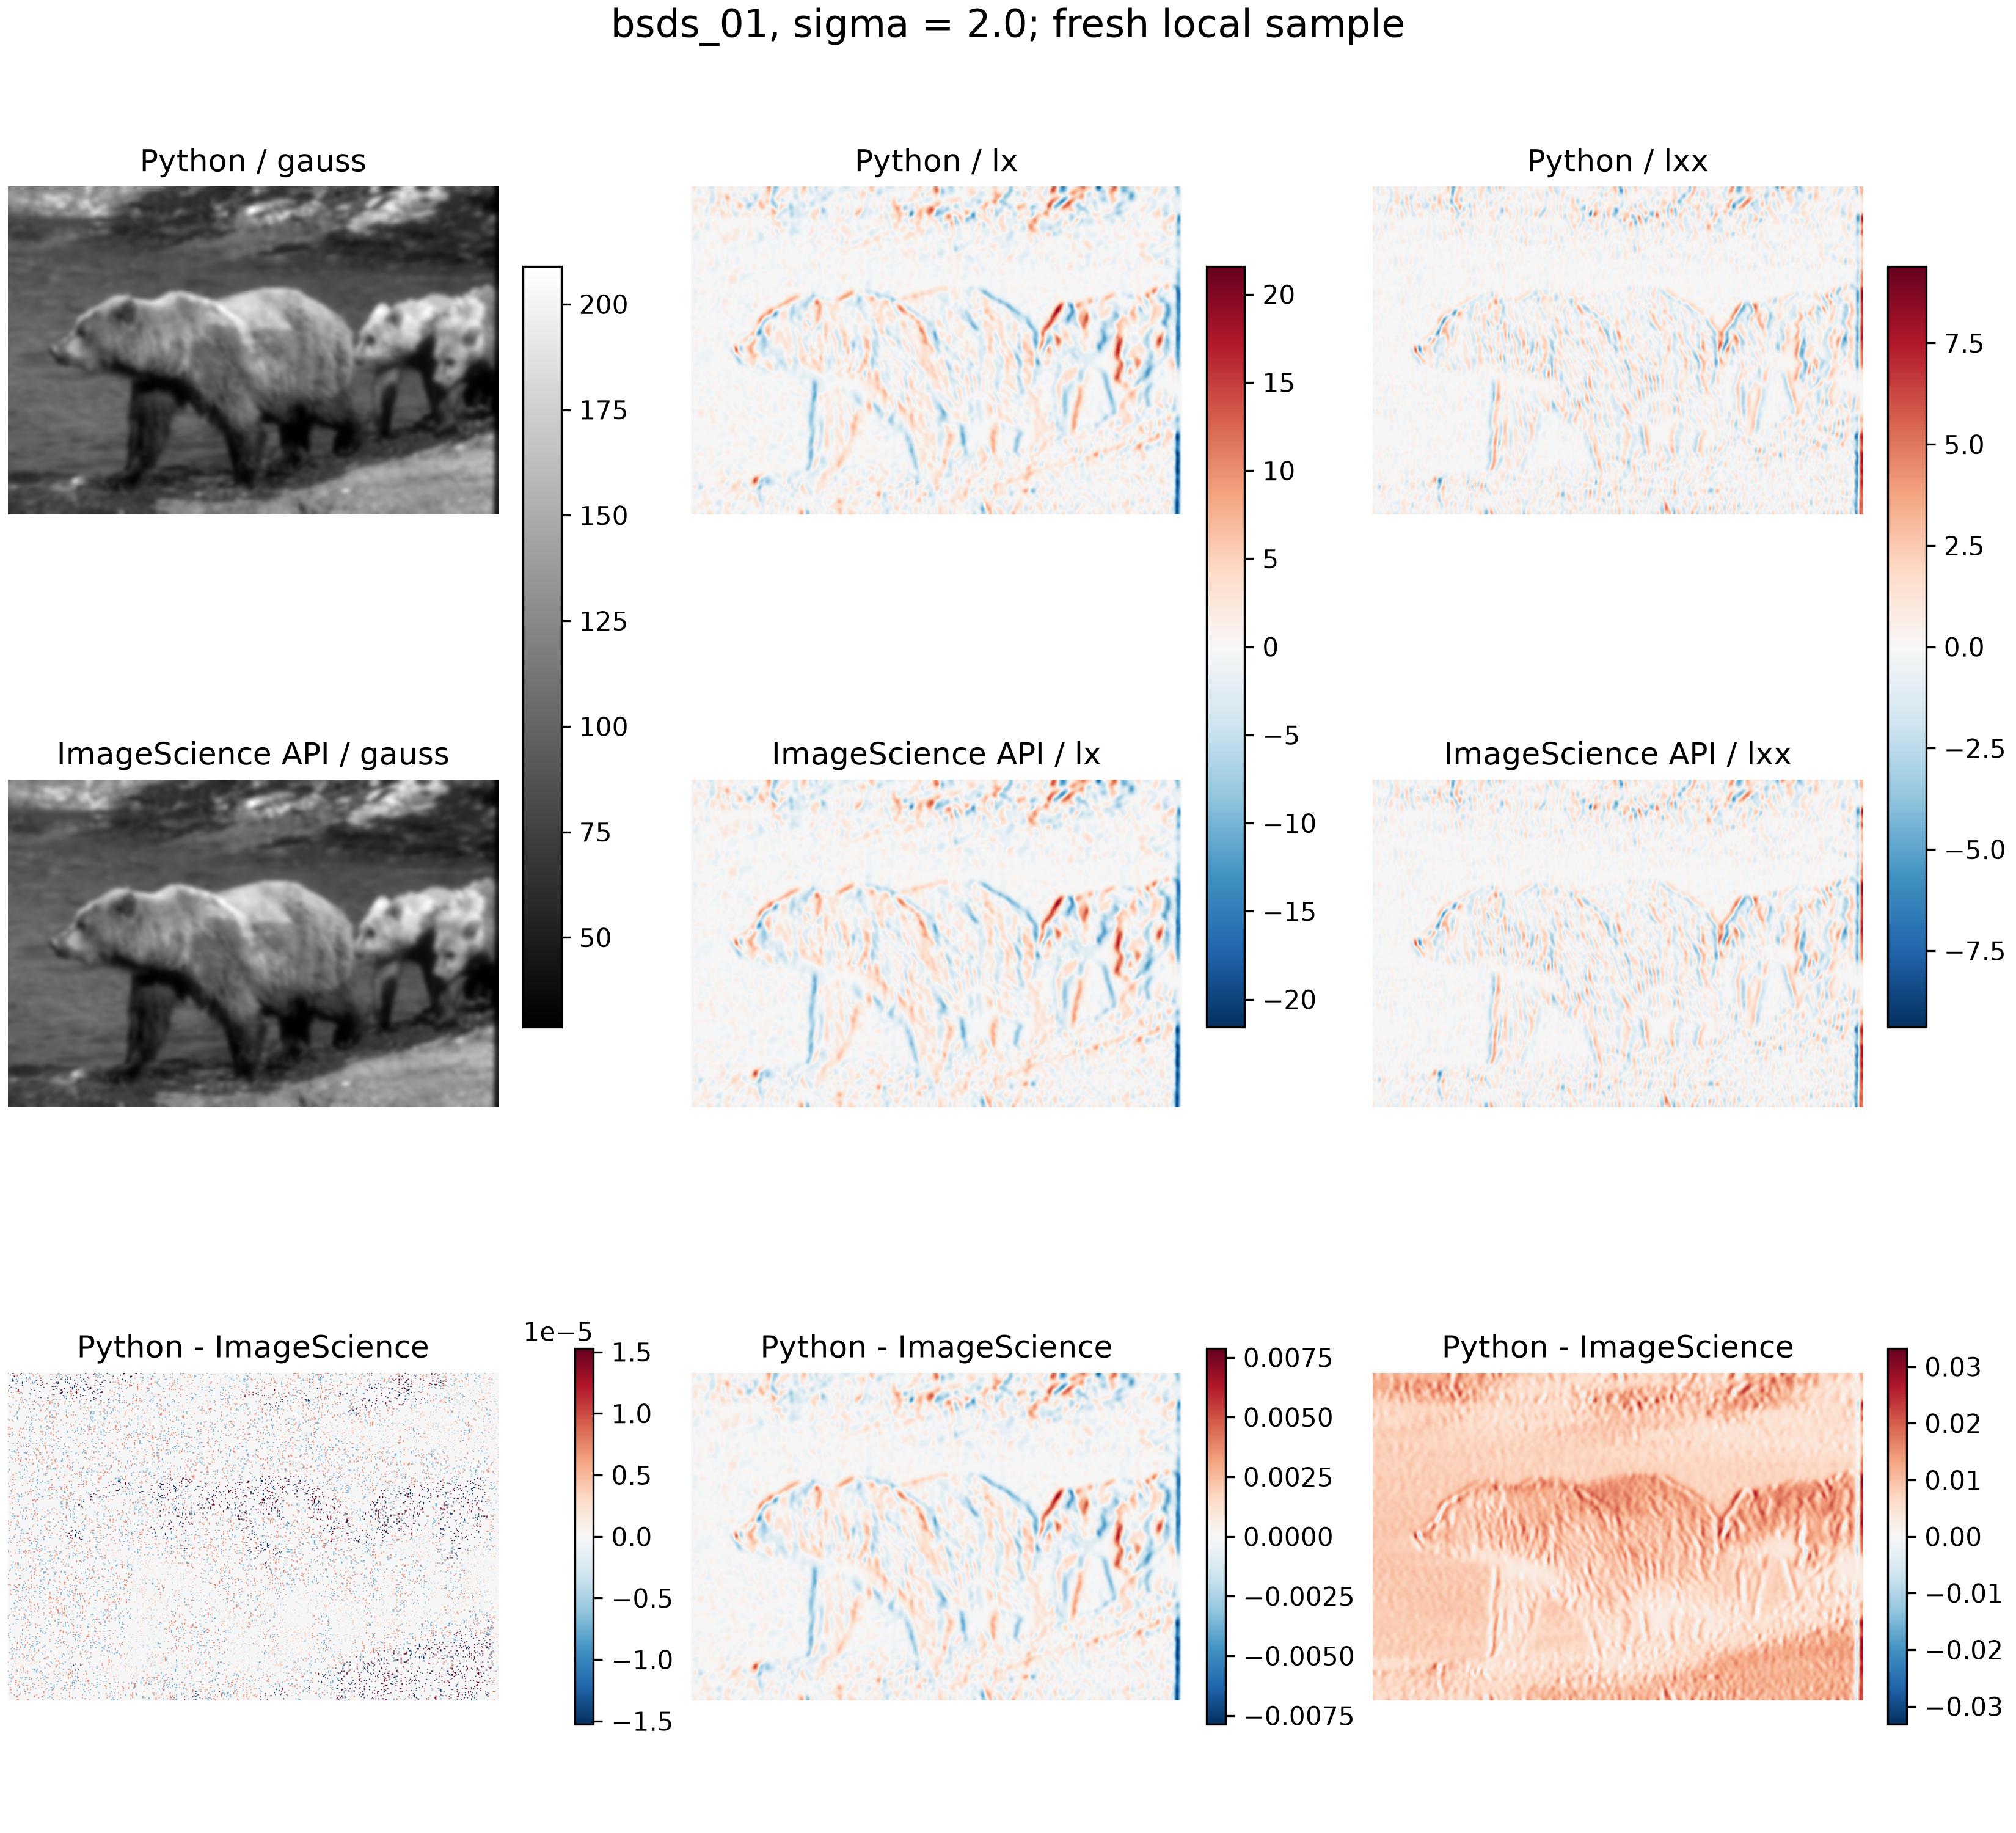
\includegraphics[width=0.82\textwidth]{figures/local_bsds_01_comparison.png}
\caption{Đối chiếu mẫu bsds\_01 tại $\sigma=2$: cột Gaussian, $L_x$, $L_{xx}$; hàng Python, ImageScience API và sai khác. Đây là dữ liệu tính mới, không phải ảnh chụp giao diện Fiji.}
\label{fig:local_bsds_01}
\end{figure*}

\begin{figure*}[tp]
\centering
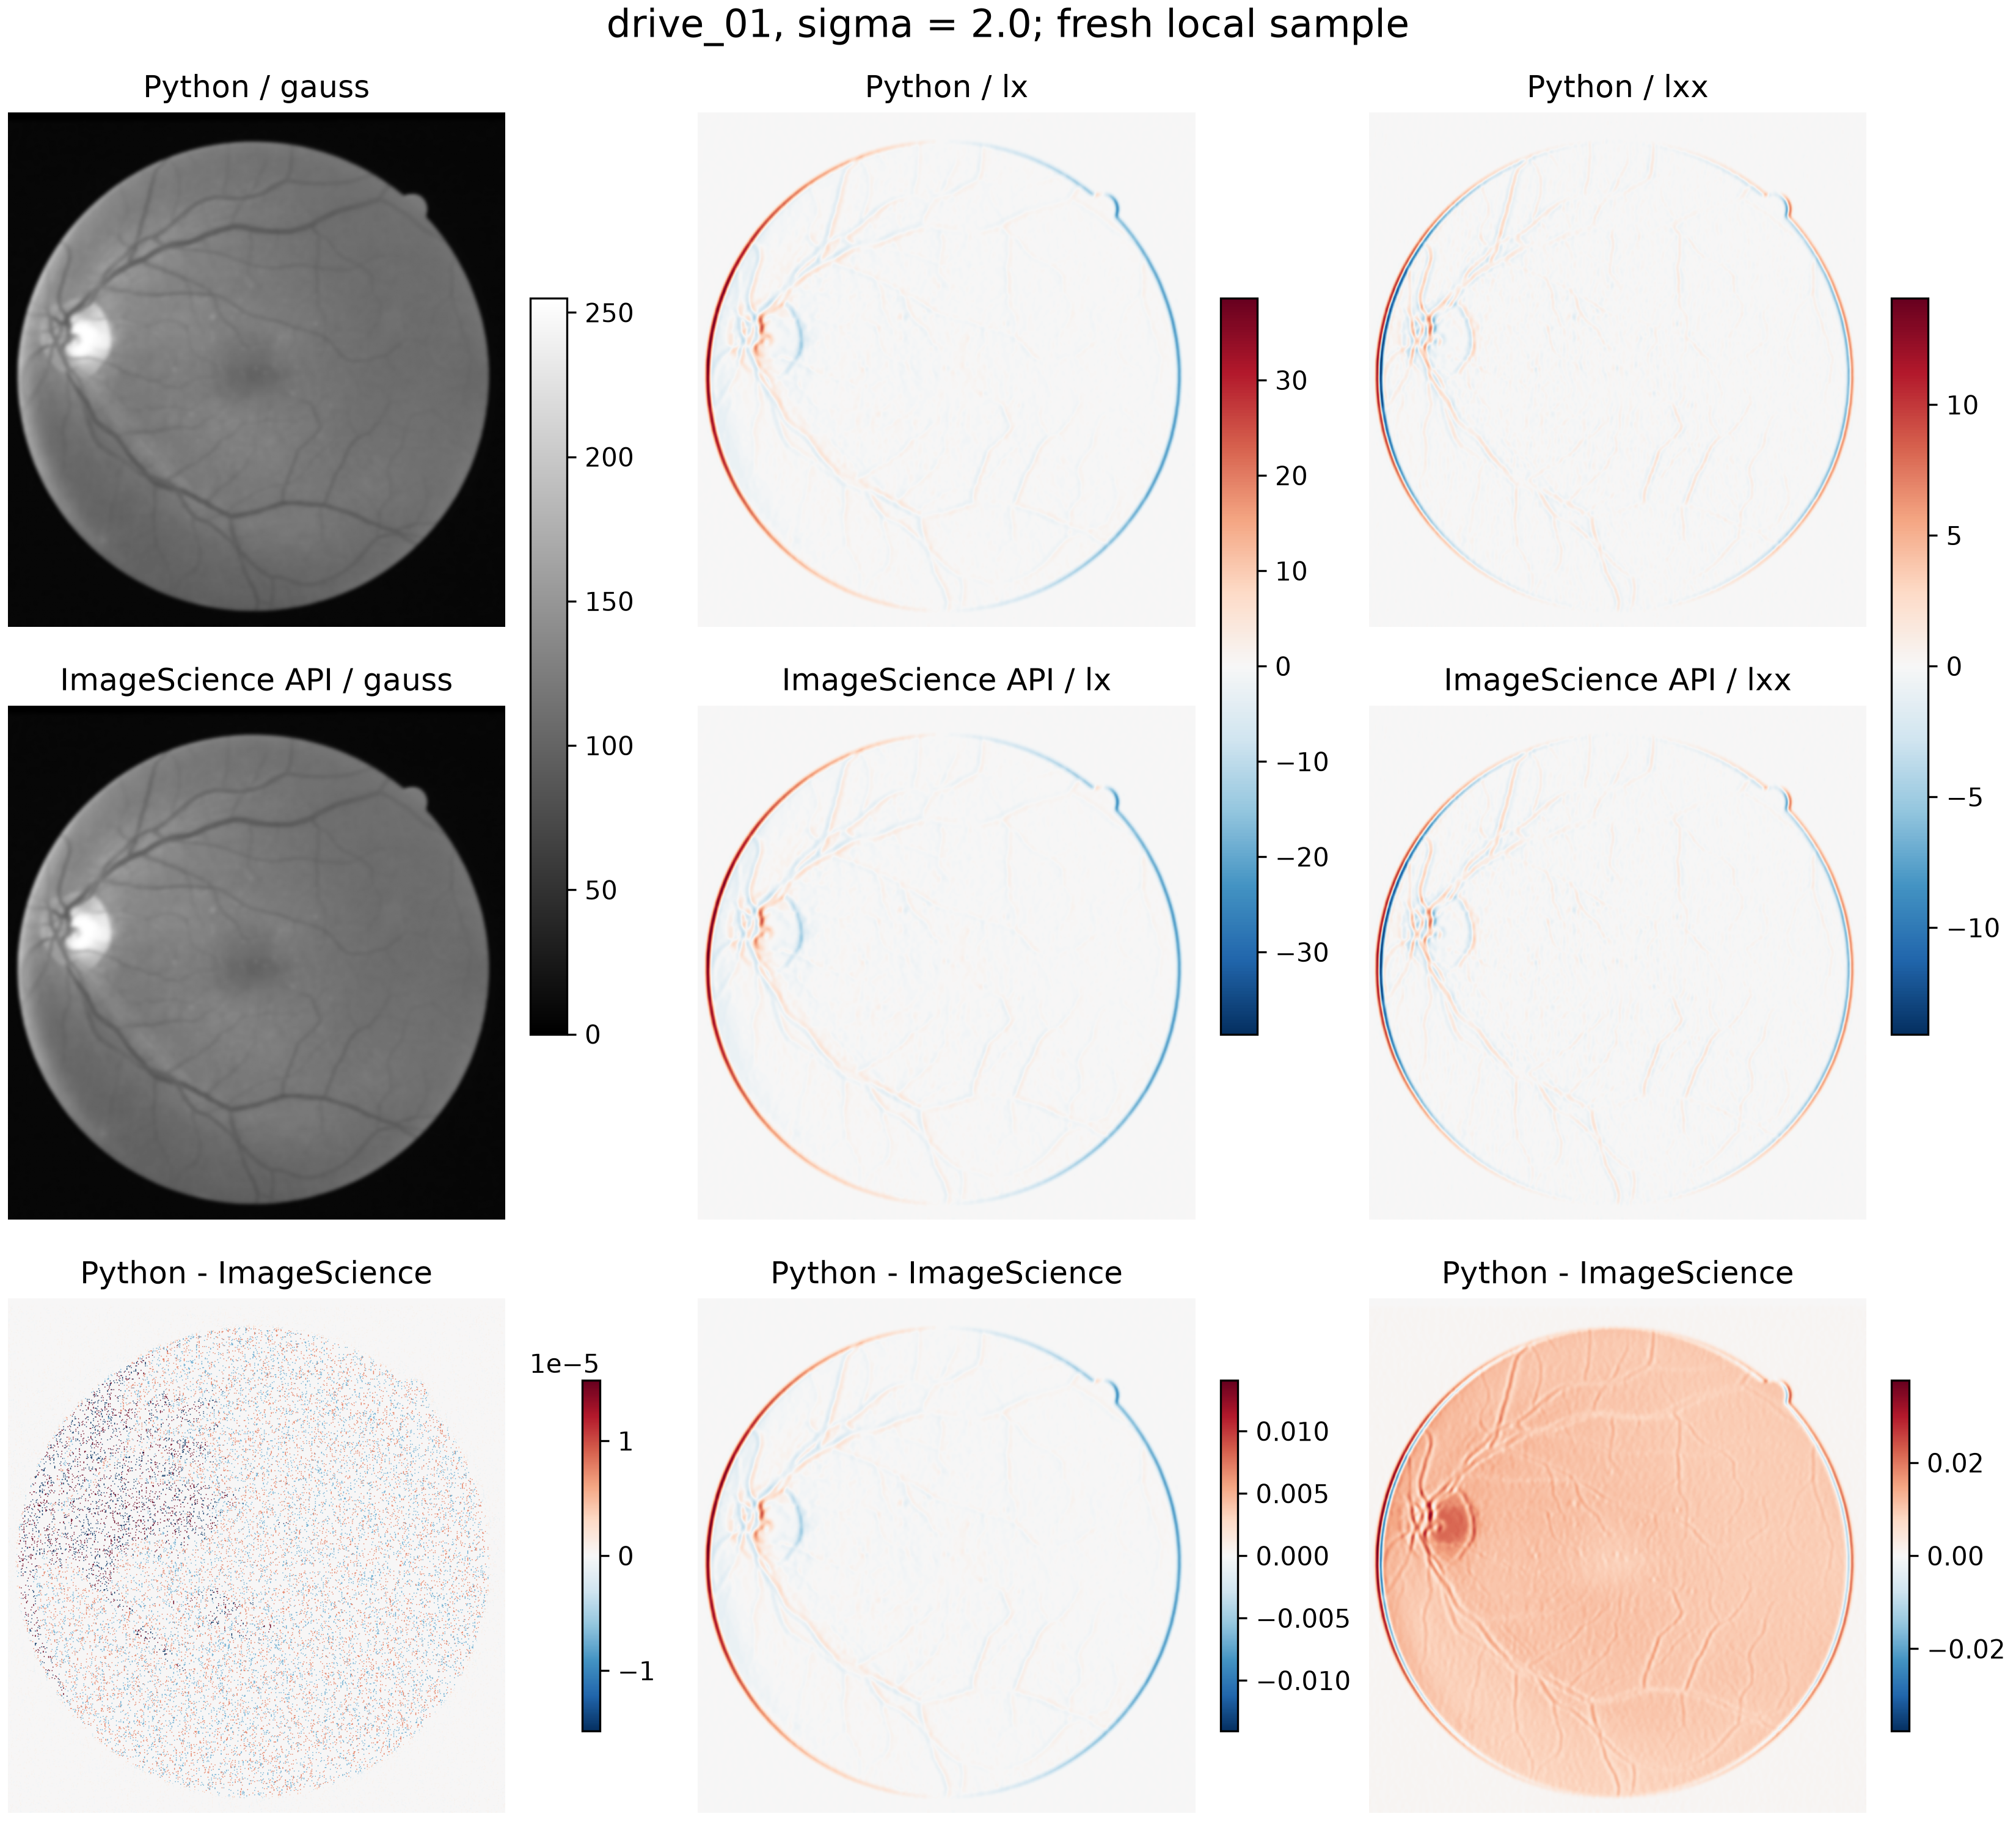
\includegraphics[width=0.82\textwidth]{figures/local_drive_01_comparison.png}
\caption{Đối chiếu mẫu drive\_01 tại $\sigma=2$: cột Gaussian, $L_x$, $L_{xx}$; hàng Python, ImageScience API và sai khác. Đây là dữ liệu tính mới, không phải ảnh chụp giao diện Fiji.}
\label{fig:local_drive_01}
\end{figure*}

\begin{figure*}[tp]
\centering
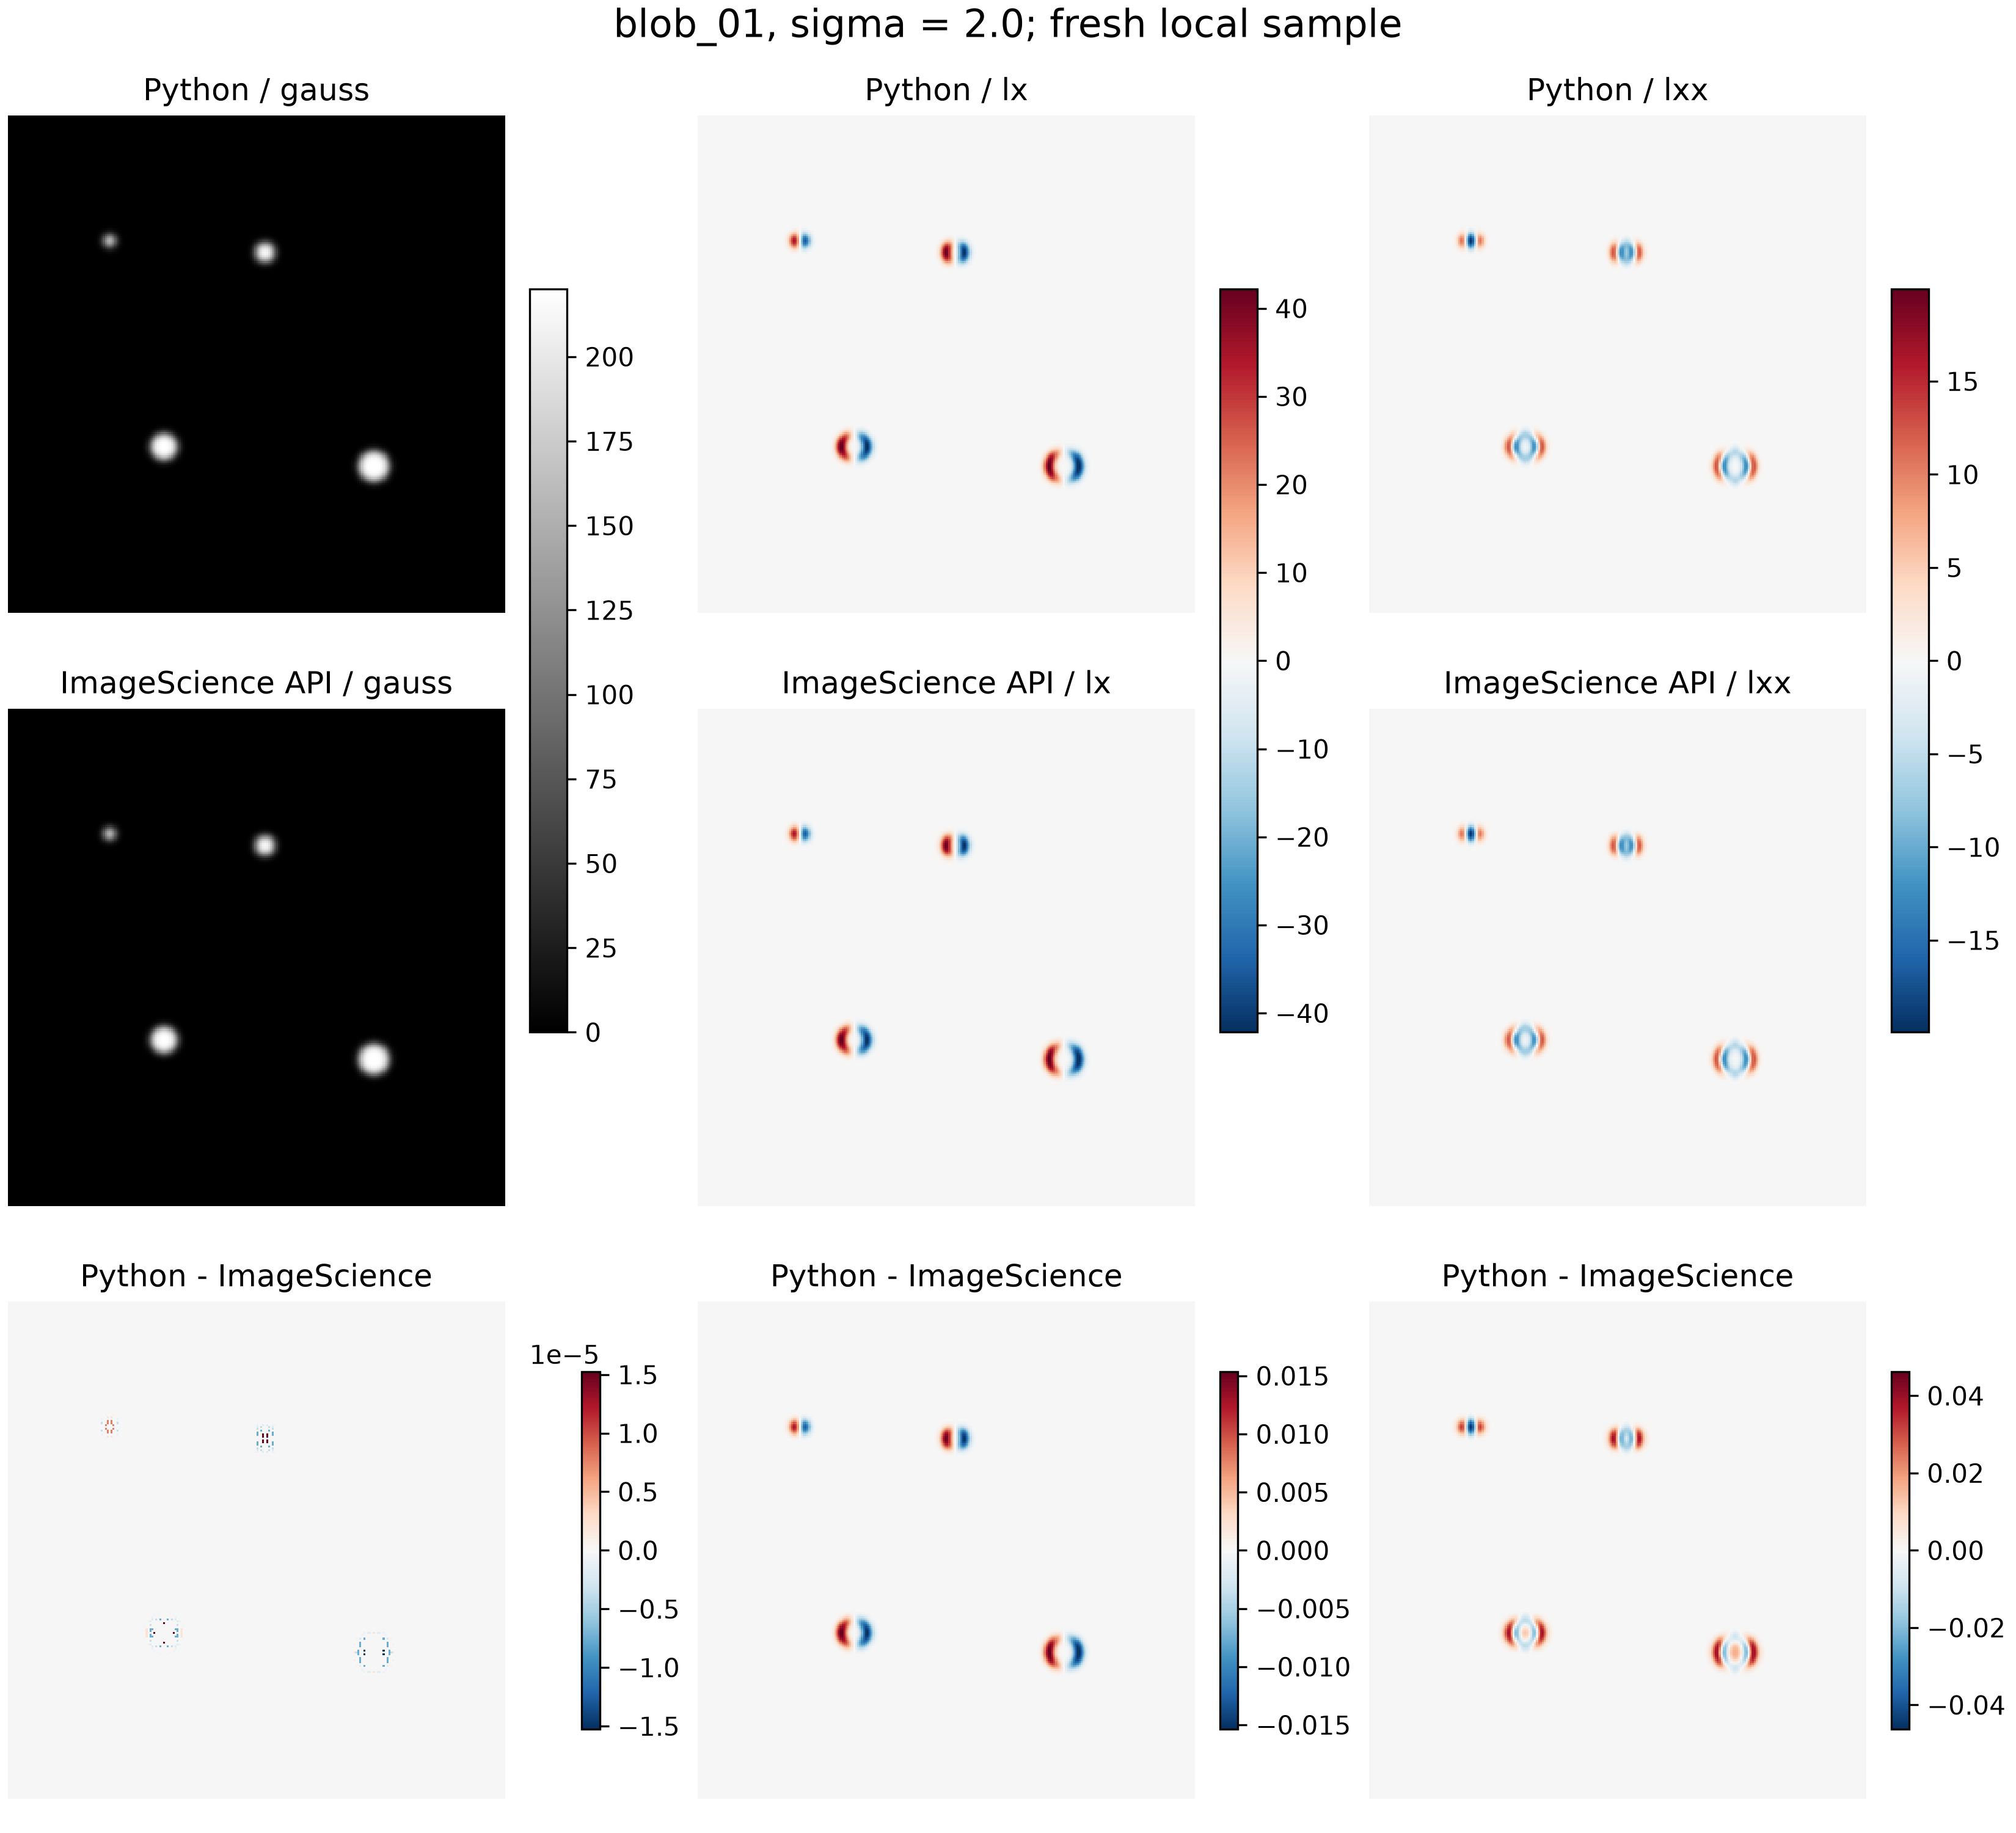
\includegraphics[width=0.82\textwidth]{figures/local_blob_01_comparison.png}
\caption{Đối chiếu mẫu blob\_01 tại $\sigma=2$: cột Gaussian, $L_x$, $L_{xx}$; hàng Python, ImageScience API và sai khác. Đây là dữ liệu tính mới, không phải ảnh chụp giao diện Fiji.}
\label{fig:local_blob_01}
\end{figure*}



\subsection{Minh chứng thực thi qua giao diện FeatureJ}
\label{sec:gui_evidence}
Bên cạnh lần xuất 72 bản đồ bằng API, một phiên GUI riêng đã được thực hiện
trên ImageJ 1.54p dùng các JAR cài trong Fiji và plugin FeatureJ build từ nguồn
chính thức. Phiên này mở các lớp plugin thật, điền điều khiển trong hộp thoại
và kích hoạt sự kiện OK bằng AWT. Vì vậy, đây là thao tác GUI được tự động hóa,
không phải các bước bấm chuột thủ công và cũng không phải hình minh họa dựng lại.
Ảnh được chụp từ cửa sổ của chính tiến trình Java bằng PrintWindow.

Mỗi phép thử đọc lại PNG gốc, chuyển sang 32-bit, đặt kích thước pixel bằng 1
và đơn vị pixel. Không dùng kết quả phép lọc trước làm đầu vào phép lọc sau.
Các tham số tỷ lệ được lấy từ config của repo. Bảng~\ref{tab:gui_parameters}
ghi cấu hình quan sát được trong các hộp thoại thật.

\begin{table*}[t]
\centering
\caption{Bốn phép thử GUI bổ sung; số đầu ra là số TIFF 32-bit đã lưu.}
\label{tab:gui_parameters}
\begin{tabular}{llp{8cm}r}
\toprule
Lệnh & Ảnh & Tham số & Đầu ra\\
\midrule
Derivatives & bsds\_01 & $x=1$, $y=z=0$, smoothing $=2$ & 1\\
Hessian & drive\_01 & smoothing $=2$; largest và smallest bật; absolute comparison tắt & 2\\
Laplacian & blob\_01 & smoothing $=2$; compute bật; zero-crossings tắt & 1\\
Structure & bsds\_01 & smoothing $=1$, integration $=3$; largest và smallest bật & 2\\
\bottomrule
\end{tabular}
\end{table*}

\begin{figure*}[t]
\centering
\begin{minipage}{0.47\textwidth}
\centering
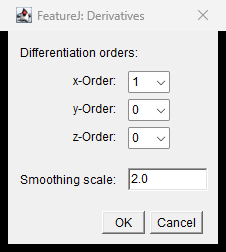
\includegraphics[height=4.6cm]{figures/gui/gui_01_derivatives_dialog.png}
\par (a) Derivatives: $L_x$, $\sigma=2$.
\end{minipage}
\hfill
\begin{minipage}{0.47\textwidth}
\centering
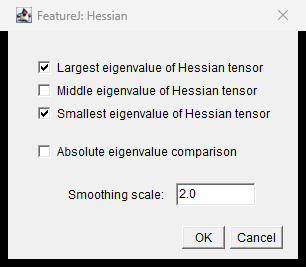
\includegraphics[height=4.6cm]{figures/gui/gui_02_hessian_dialog.png}
\par (b) Hessian: giữ dấu trị riêng.
\end{minipage}
\par\medskip
\begin{minipage}{0.47\textwidth}
\centering
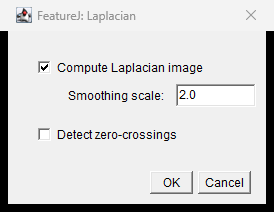
\includegraphics[height=4.3cm]{figures/gui/gui_03_laplacian_dialog.png}
\par (c) Laplacian: không lấy zero-crossings.
\end{minipage}
\hfill
\begin{minipage}{0.47\textwidth}
\centering
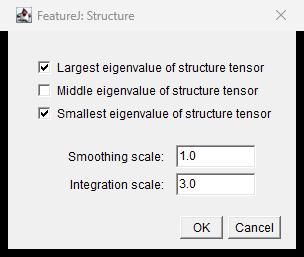
\includegraphics[height=4.3cm]{figures/gui/gui_04_structure_dialog.png}
\par (d) Structure: hai tỷ lệ khác nhau.
\end{minipage}
\caption{Bốn hộp thoại FeatureJ thật trong phiên GUI bổ sung. Các lựa chọn
được đặt trước khi kích hoạt OK; không sử dụng ảnh vẽ lại giao diện.}
\label{fig:gui_dialogs}
\end{figure*}

\begin{figure}[htbp]
\centering
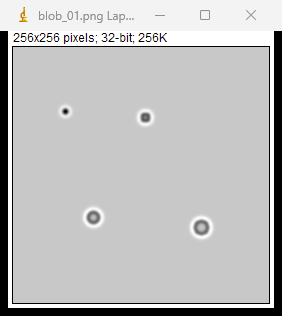
\includegraphics[width=0.72\columnwidth]{figures/gui/gui_03_laplacian_result.png}
\caption{Kết quả Laplacian thật trên blob\_01 tại $\sigma=2$.
Các đốm và vòng đổi dấu minh họa đáp ứng bậc hai; ảnh này chưa phải
kết quả phát hiện blob đa tỷ lệ hoặc kết quả ghép với Ground Truth.}
\label{fig:gui_laplacian}
\end{figure}

Nhật ký \texttt{gui\_capture\_log.csv} ghi bốn lệnh, tham số, thời điểm UTC,
số đầu ra và phương thức chụp. Tổng cộng có sáu TIFF 32-bit trong
\texttt{Code/experiments/gui\_evidence}. Chúng tách khỏi
\texttt{sample\_local}, nơi lưu 72 cặp dùng để chấm sai số.
Phiên GUI xác nhận plugin nhận đúng cấu hình và tạo kết quả;
nó không bổ sung một benchmark F1 mới và không thay thế bộ đối chiếu API.
Đầu ra Derivatives và Laplacian ở đây chưa nhân hệ số chuẩn hóa theo tỷ lệ;
khi đối chiếu với bản đồ đã chuẩn hóa phải áp dụng cùng quy ước
$\sigma^n$ cho đạo hàm bậc $n$.


Đối chiếu TIFF GUI với API trên toàn ảnh cho $L_x$ sai số cực đại bằng 0;
Laplacian so với tổng $L_{xx}+L_{yy}$ có sai số cực đại
$1.90735\times10^{-6}$ và RMSE $4.18613\times10^{-8}$.
Đây là kiểm tra hai phép thử cùng thư viện, không phải so sánh độc lập với NumPy.


\subsection{Ảnh hưởng của tỷ lệ đến kết quả BSDS500}
\begin{table*}[t]
\centering
\caption{Kết quả BSDS500 canonical theo tỷ lệ: ngưỡng chọn trên Python và giữ cho Fiji; dung sai là đĩa Euclidean bán kính 2 px, còn FeatureJ Edges là pipeline tham chiếu riêng}
\begin{tabular}{crrrrr}
\toprule
$\sigma$ & $p_l/p_h$ & Python F1 & Fiji fair F1 & $\Delta F_1$ & FeatureJ Edges F1\\
\midrule
1 & 76/94 & 0.455418 & 0.455478 & 0.000060 & 0.488766\\
2 & 67/91 & 0.477886 & 0.477886 & 0.000000 & 0.500818\\
4 & 49/80 & 0.441491 & 0.441491 & 0.000000 & 0.464873\\
8 & 23/50 & 0.343340 & 0.343340 & 0.000000 & 0.354292\\
\bottomrule
\end{tabular}
\label{tab:bsds_scales_detailed}
\end{table*}
Bảng~\ref{tab:bsds_scales_detailed} cho thấy $\sigma=2$ tốt nhất trong bốn mức đã khảo sát, với điều kiện bộ ngưỡng được chọn riêng tại mỗi mức \cite{xlaRepository}. Kết quả này không chứng minh $\sigma=2$ tối ưu cho mọi ảnh: độ phân giải, kích thước đối tượng và tiêu chí nhãn đều có thể thay đổi tỷ lệ thích hợp.

Ở $\sigma=1$, nhiều chi tiết kết cấu còn rõ nên số ứng viên biên có thể nhiều hơn. Ở $\sigma=8$, các biên nhỏ có thể mất, các đường gần nhau có thể nhập lại, làm khả năng khớp nhãn giảm. Mức trung gian đạt cân bằng tốt hơn trên tập đang dùng. Vì cả $\sigma$ và ngưỡng đều thay đổi trong bảng, không quy toàn bộ chênh lệch F1 cho riêng độ làm mịn.

Các điểm fair gần như trùng nhau cho thấy thay nguồn đạo hàm trong cùng bộ hậu xử lý chỉ làm thay đổi nhỏ điểm số ở cấu hình này. Cột FeatureJ Edges có điểm khác vì sử dụng NMS và ngưỡng theo nhánh tham chiếu riêng. Không dùng cột này để kết luận một nhân đạo hàm tốt hơn nhân còn lại.

\subsection{Cách đọc sai khác giữa các bản đồ}
Nếu hai bản đồ có Pearson gần 1 nhưng $E_{\mathrm{rel}}$ khác 0, trước hết kiểm tra hệ số tỷ lệ: chuẩn hóa $\sigma^n$, chuẩn moment và miền cường độ. Nếu chỉ sai vùng gần mép ảnh, kiểm tra bán kính hỗ trợ và kiểu đệm. Nếu sai khác có cấu trúc bị xoay hoặc hoán đổi hướng, kiểm tra trục x/y. Nếu đạo hàm bậc lẻ đổi dấu trên hầu hết ảnh còn bậc chẵn gần trùng, kiểm tra tích chập so với tương quan.

Hình sai khác nên được biểu diễn từ $D=P-F$ với thang màu đối xứng quanh 0; đồng thời cung cấp $|D|$ khi cần xem độ lớn lỗi. Tự động giãn thang màu riêng cho mỗi bản đồ có thể làm hai đầu ra khác biên độ trông giống nhau. Ngược lại, một bản đồ sai khác có màu rực không nhất thiết mang sai số lớn nếu thang hiển thị rất hẹp.

\subsection{Các tình huống lỗi dự kiến và cách giải thích}
\begin{table*}[t]
\centering
\caption{Tình huống cần phân tích trên hình và các giả thuyết cần kiểm tra}
\begin{tabularx}{\textwidth}{lXX}
\toprule
Bài toán & Biểu hiện quan sát & Cách kiểm tra và diễn giải\\
\midrule
Biên & Nhiều nét ở vùng kết cấu & Kiểm tra ngưỡng, mức làm mịn và nhãn đường bao; chưa đủ cơ sở quy cho lỗi đạo hàm\\
Biên & Biên bị ngắt hoặc mất chi tiết & Kiểm tra ngưỡng cao, $\sigma$ lớn và liên thông hysteresis\\
Mạch & Viền FOV sáng hơn mạch & Kiểm tra mặt nạ và vùng tính điểm, tránh tăng ngưỡng chỉ để che lỗi viền\\
Mạch & Mất mạch nhỏ hoặc dính vùng giao & Kiểm tra lưới tỷ lệ, ngưỡng và hạn chế mô hình ridge cục bộ\\
Blob & Nhiều vòng quanh một đối tượng & Kiểm tra cực trị 3D, plateau và khử trùng theo vị trí/kích thước\\
Blob & Tâm đúng nhưng không được ghép & Kiểm tra ngưỡng sai số bán kính và tính không chắc chắn của nhãn\\
\bottomrule
\end{tabularx}
\end{table*}
Các dòng trong bảng là giả thuyết phân tích, không phải thống kê lỗi đã được đo riêng trên tập dữ liệu. Muốn kết luận nguyên nhân, cần chọn ví dụ thực tế, lưu cấu hình và thay đổi một yếu tố có kiểm soát.

\subsection{Giới hạn và thiết kế thí nghiệm tiếp theo}
Thứ nhất, tập đánh giá nhỏ: 10 ảnh mỗi bộ BSDS500 và DRIVE, cùng 5 ảnh Blob. Các giá trị trung bình mô tả tập con đang dùng; chưa có cơ sở coi chúng là hiệu năng trên toàn bộ dữ liệu hoặc ảnh chụp trong điều kiện khác.

Thứ hai, ngưỡng BSDS được lựa chọn và đánh giá trên cùng ảnh. Một thiết kế chặt chẽ hơn cần tách tập chọn tham số và tập đánh giá cuối, cố định $\sigma$, ngưỡng và các tham số Frangi/LoG trước khi xem nhãn tập cuối. Khi đó điểm số có thể giảm nhưng phản ánh khả năng tổng quát hóa rõ hơn.

Thứ ba, nhãn đa annotator, độ rộng mạch do người vẽ và bán kính tế bào đều có sai khác chủ quan. Báo cáo dung sai ghép và phân tích ảnh lỗi giúp người đọc hiểu ý nghĩa của TP/FP/FN, thay vì coi nhãn là một mô hình hình học hoàn toàn chính xác.

Thứ tư, chưa có khoảng tin cậy hay phép kiểm định thống kê cho chênh lệch F1 rất nhỏ. Các chênh lệch khoảng $10^{-3}$ được dùng như mô tả tính nhất quán của hai pipeline trên tập này, không phải bằng chứng về khác biệt chất lượng có ý nghĩa thống kê.

Thứ năm, thời gian chạy chỉ có ý nghĩa khi cùng phạm vi công việc: đọc/ghi ảnh, khởi động JVM, thời gian plugin và hậu xử lý phải được xác định rõ. Cần bỏ lần khởi động, chạy lặp lại, báo cáo trung vị và phần cứng thực tế. Vì chưa tái chạy phép đo trên máy biên tập, bản báo cáo không thêm một hệ số tăng tốc mới từ suy luận độ phức tạp.

Cuối cùng, ảnh Blob tổng hợp giúp kiểm tra đúng đắn hình học nhưng có hình dạng và nền đơn giản. Khoảng cách giữa F1=1 trên ảnh tổng hợp và F1 khoảng 0.465 trên ảnh sinh học nhấn mạnh nhu cầu đánh giá trên cấu trúc chồng lấp, nền không đều và nhiều dạng kích thước.


\subsection{Cập nhật tài liệu và phân tích từ repo đến commit \texttt{58bdfd8}}
\label{sec:repo-update}
Từ commit \texttt{58e28e7} dùng trong lần chạy mẫu đến \texttt{950d47f},
bốn commit bổ sung tài liệu workflow Fiji, kiểm kê Ground Truth và bộ
phân tích công việc 5 của Đức \cite{xlaUpdate950}. Các đầu ra này cung cấp
bối cảnh thực nghiệm và quy trình bàn giao; chúng không thay thế bộ metric
Tầng 2 chuẩn. Hai commit mới nhất sau snapshot trước đã thay đổi giao thức
đánh giá: \texttt{50f65e1} đổi dung sai BSDS từ ô vuông $5\times5$ sang
đĩa Euclidean bán kính 2 pixel (13 pixel), chuyển phép hình thái học trong
bộ đánh giá sang NumPy thuần và giữ ảnh NMS rỗng trong mẫu số với $F_1=0$.
Commit \texttt{58bdfd8} tái tạo số liệu Tier 2 và đồng bộ tài liệu, biểu đồ
và cấu hình theo giao thức mới. Thư mục \texttt{outputs/metrics/duc\_08\_11}
được đánh dấu là snapshot lịch sử trước khi sửa dung sai; nguồn canonical
hiện tại là \texttt{outputs/metrics/PROTOCOL.md} và các CSV cùng thư mục.

\subsubsection{Rà soát trạng thái các nhánh ngày 10/11/2026}
GitHub liệt kê bốn nhánh từ xa. \texttt{dev/NguyenDucManh} đứng tại
\texttt{58bdfd8} và là nguồn canonical hiện hành; \texttt{main} chậm hơn
năm commit và \texttt{fiji/PhamBaoLoc} chậm hơn chín commit. Nhánh
\texttt{thucnghiem/BuiTrungDuc} phân nhánh từ lịch sử cũ, có hai commit
riêng nhưng chậm hơn \texttt{dev} 45 commit; snapshot metric của nhánh này
không thay thế giao thức canonical mới. Nhánh báo cáo
\texttt{report/ieee-gaussian-39e4d02} chỉ có trong checkout cục bộ tại
commit \texttt{a29b82e}; chưa có nhánh cùng tên trên GitHub.

\subsubsection{Phạm vi batch Fiji theo tài liệu mới}
Theo tài liệu workflow đã cập nhật, kho đầu ra Fiji có 435 TIFF float32:
423 bản đồ thuộc phạm vi macro hiện hành và 12 tệp Edge legacy. Nhật ký
có 369 dòng, gồm 303 lệnh một đầu ra và 66 lệnh hai đầu ra; trong số
303 dòng một đầu ra có 12 dòng legacy. Vì vậy phạm vi macro hiện hành
gồm 357 lần gọi và 423 TIFF. Hessian có 14 ảnh, bốn tỷ lệ và hai trị riêng,
tương ứng 56 lần gọi và 112 TIFF. Macro bỏ qua tệp đã có và validator được
chạy riêng sau batch; những con số kiểm kê này không chứng minh mọi TIFF
đã được tạo mới trong cùng một lần chạy.

\subsubsection{Kiểm kê Ground Truth}
Theo tài liệu bàn giao ngày 09/11, mười ảnh BSDS được giữ riêng
5--7 bộ nhãn trên mỗi ảnh, tổng cộng 56 bộ nhãn theo ảnh; con số 56
không đồng nghĩa với 56 người khác nhau. Mỗi ảnh DRIVE có nhãn mạch và
mặt nạ trường quan sát (FOV) riêng. Bốn ảnh blob tổng hợp có bốn đối tượng
mỗi ảnh. Ảnh tế bào \texttt{blob\_05} có 276 đối tượng dương tính đã duyệt
và 15 vùng hình chữ nhật loại trừ; dự đoán có tâm nằm trong vùng loại trừ
được bỏ khỏi ghép nhãn và phép đếm FP theo giao thức tài liệu bàn giao.
Nhãn tế bào do nhóm xây dựng, có gợi ý và kiểm duyệt thủ công; không
xem đây là nhãn chuyên gia chính thức của nhà cung cấp dữ liệu.

\begin{figure*}[tp]
\centering
\begin{minipage}{0.47\textwidth}
\centering
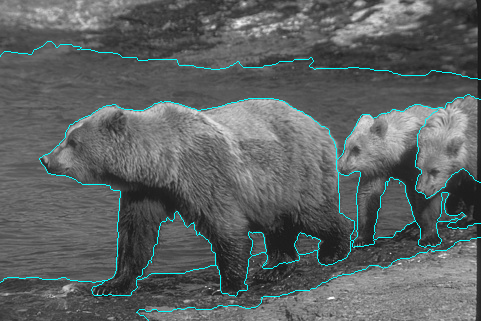
\includegraphics[width=\linewidth]{figures/gt_bsds_01_overlay.png}
\par (a) Biên của một người gán nhãn trên ảnh BSDS.
\end{minipage}
\hfill
\begin{minipage}{0.47\textwidth}
\centering
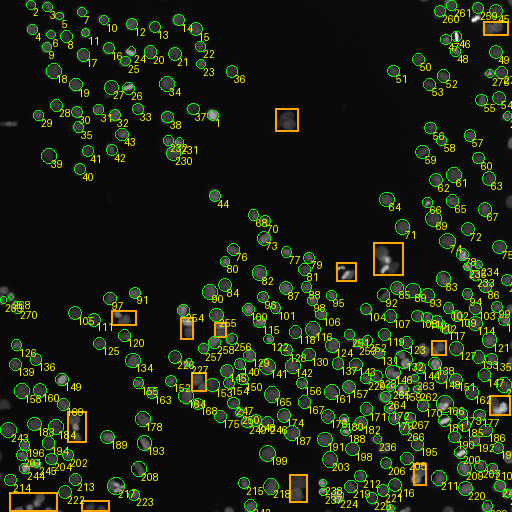
\includegraphics[width=\linewidth]{figures/gt_blob_05_overlay.png}
\par (b) Tâm, bán kính và vùng loại trừ trên ảnh tế bào.
\end{minipage}
\caption{Minh họa Ground Truth do nhóm cung cấp trong
\texttt{docs/09\_11/ground\_truth\_figures}: đường cyan ở (a) là nhãn
của annotator 01 trong sáu bộ nhãn của ảnh; vòng xanh và khung cam ở (b)
biểu diễn đối tượng và vùng loại trừ. Overlay dùng để minh họa,
không được thay thế mask hoặc JSON gốc khi tính chỉ số.}
\label{fig:gt-handoff}
\end{figure*}

\subsubsection{Số liệu Tầng 2 theo giao thức canonical hiện tại}
Commit \texttt{58bdfd8} tái tạo metric trong \texttt{outputs/metrics/}
theo dung sai đĩa Euclidean. Các F1 BSDS dưới đây và cặp ngưỡng lấy từ
\texttt{PROTOCOL.md}; bảng Python--Fiji DRIVE/Blob và số đếm micro lấy từ
\texttt{tier2\_results\_both.csv}. Kết quả Python Blob chính thức ở lưới
8 mức được lưu riêng trong \texttt{tier2\_results.csv}.

\begin{table*}[htbp]
\centering
\caption{F1 theo bộ metric canonical tại commit \texttt{58bdfd8}.}
\label{tab:repo-canonical-f1}
\begin{tabular}{lrrr}
\toprule
Tác vụ / tỷ lệ & Python & Fiji & $\Delta F_1$\\
\midrule
BSDS $\sigma=1$ & 0.455418 & 0.455478 & $+0.000060$\\
BSDS $\sigma=2$ & 0.477886 & 0.477886 & $0.000000$\\
BSDS $\sigma=4$ & 0.441491 & 0.441491 & $0.000000$\\
BSDS $\sigma=8$ & 0.343340 & 0.343340 & $0.000000$\\
DRIVE, macro & 0.680633 & 0.681651 & $+0.001019$\\
DRIVE, micro & 0.682895 & 0.683897 & ---\\
Blob, macro & 0.893023 & 0.891901 & $-0.001122$\\
Blob, micro & 0.492114 & 0.486656 & ---\\
\bottomrule
\end{tabular}
\end{table*}

Với BSDS $\sigma=\{1,2,4,8\}$, cặp $(p_{low},p_{high})$ lần lượt là
$(76,94)$, $(67,91)$, $(49,80)$ và $(23,50)$; F1 tham chiếu FeatureJ Edges
lần lượt là $0.488766$, $0.500818$, $0.464873$ và $0.354292$. Ngưỡng được
chọn trên Python rồi giữ nguyên cho Fiji, nên đây không phải điểm kiểm tra
độc lập. DRIVE được chấm trong FOV đã xói mòn $\lceil4\sigma\rceil$.
Blob dùng ghép một-một, tâm trong 2 pixel, bán kính sai không quá 20%, và
bỏ dự đoán có tâm trong vùng ignore. Bảng macro Python--Fiji dùng cấu hình
chung 7 mức. Riêng kết quả Python chính thức cho \texttt{blob\_05} ở lưới
8 mức là 140/329 ghép đúng/dự đoán ($F_1=0.4628$); Fiji fair 7 mức là
139/329 ($F_1=0.4595$). Hàng Python 7 mức 140/326 ($F_1=0.4651$) vẫn có
trong CSV so sánh lưới chung, nhưng không phải kết quả Python chính thức
dùng làm headline. Các micro F1 được tính từ tổng số đếm trong CSV.

\subsubsection{Hiệu quả chập tách rời}
Benchmark đo chập 2D trực tiếp so với hai chập 1D tách rời cho Gaussian,
$L_x$ và $L_{xx}$, trên ba ảnh mẫu và bốn tỷ lệ, tổng cộng 36 trường hợp với
5 lần lặp mỗi trường hợp. Theo CSV
\texttt{outputs/metrics/optimization\_benchmark.csv}, tốc độ nhanh hơn
nằm trong khoảng $1.375738$ đến $31.392971$ lần tùy ảnh, tỷ lệ và toán tử;
sai khác tuyệt đối lớn nhất là $1.279\times10^{-12}$
\cite{xlaOptimizationBenchmark}. Mức tăng tốc quan sát
không cần bằng đúng tỷ số số phép toán lý thuyết: phép đo còn chịu ảnh hưởng
của kích thước kernel, overhead Python và quản lý bộ nhớ. Đây là benchmark
trên ba ảnh mẫu, không phải cam kết tốc độ trên toàn bộ dữ liệu hay máy khác.

\subsubsection{Cấu hình FeatureJ Derivatives}
Tài liệu Fiji mới ghi tham số hệ số cắt kernel $k=3$ cho Gaussian và
$k=4$ cho đạo hàm bậc 1--2, biên phản chiếu \texttt{mirror}, và đầu ra
FeatureJ là giá trị thô, không nhân thêm $\sigma^n$. Vì đây là quy ước
riêng được ghi trong workflow hiện tại, cần nêu rõ khi tái lập hoặc so với
nhánh NumPy có chuẩn hóa tỷ lệ; không được coi ảnh chụp GUI là phép xác nhận
độc lập cho toàn bộ benchmark.

\subsubsection{Tiêu chí nghiệm thu Tầng 1}
Trong metric snapshot mới, 35/220 cặp đạt đồng thời ngưỡng gốc
$\mathrm{rel\_err}<10^{-4}$ và Pearson $>0.9999$; 185 cặp còn lại
\emph{chưa đạt ngưỡng gốc}. Các nhãn \texttt{RELAXED} trong snapshot trước
chỉ mô tả kết quả theo ngưỡng nới lỏng của báo cáo, không phải xác nhận
nhóm đã chấp nhận thay đổi tiêu chí nghiệm thu. Tương quan cao không đủ
để kết luận sai số biên độ thỏa chuẩn.



\section{Chương 6: Kết Luận và Hướng Phát Triển}

\subsection{Tổng Kết Các Kết Quả Chính}
Đề tài xây dựng một pipeline phân tích đặc trưng đa tỷ lệ bằng đạo hàm Gaussian, gồm nhân NumPy, bản đồ tham chiếu FeatureJ và bộ đánh giá theo Ground Truth. Các kết quả chính:
\begin{enumerate}
    \item \textbf{Đối chiếu số học:} 220 bản đồ gồm 35 đạt ngưỡng gốc và 185 chưa đạt ngưỡng gốc, dù các bản đồ này nằm trong mức \texttt{RELAXED} để tham khảo; Pearson trung bình là $0.99999710$. Sai số tương đối bậc hai khoảng $0.3$--$0.4\%$, vì vậy tương quan cao không được đồng nhất với sai số bằng không.
    \item \textbf{Đánh giá tác vụ:} Python đạt $F_1=0.477886$ trên BSDS500 tại $\sigma=2$ và $F_1=0.680633$ trên DRIVE ($IoU=0.5184$). Macro-$F_1$ Blob là $0.893023$ (Python) và $0.891901$ (Fiji); riêng \texttt{blob\_05}, Python 8 mức đạt $0.4628$.
    \item \textbf{Đối chiếu Python--Fiji:} Theo metric snapshot canonical tại commit \texttt{58bdfd8}, F1 macro Python--Fiji lần lượt là $0.477886/0.477886$ ở BSDS $\sigma=2$, $0.680633/0.681651$ trên DRIVE và $0.893023/0.891901$ trên Blobs. Đây là kết quả của pipeline và tập ảnh đã chọn, không phải bằng chứng rằng một nguồn vượt trội hoặc điểm kiểm tra độc lập.
    \item \textbf{Tối ưu tích chập:} Benchmark 36 trường hợp, 5 lần lặp, đo mức tăng tốc $1.375738$--$31.392971$ lần cho tích chập tách rời so với tích chập 2D trực tiếp; sai khác tối đa là $1.279\times10^{-12}$. Đây là số đo trên ba ảnh mẫu, không phải bảo đảm cho mọi ảnh hay máy tính.
    \item \textbf{Giới hạn:} Kết quả phụ thuộc vào lưới tỷ lệ, ngưỡng, tiêu chí ghép và bộ nhãn. Đặc biệt, blob tổng hợp không đại diện đầy đủ cho độ khó của ảnh sinh học.
\end{enumerate}
\subsection{Bài Học Kinh Nghiệm}
Quá trình nghiên cứu và triển khai gợi ra hai điểm cần lưu ý:
\begin{itemize}
    \item \textbf{Tầm quan trọng của điều kiện bảo toàn moment rời rạc:} Không thể lấy mẫu hàm Gaussian liên tục một cách tùy tiện trên lưới điểm rời rạc. Việc thỏa mãn các điều kiện moment Taylor là chìa khóa để bảo toàn đặc tính vi phân giải tích.
    \item \textbf{Xử lý hiệu ứng biên trong không gian đa tỷ lệ:} Ở các tỷ lệ lớn ($\sigma \ge 4.0$), hạt nhân lọc có kích thước lên tới hàng chục pixel. Việc thiết lập chiến lược xói mòn mặt nạ thích ứng là bắt buộc để ngăn chặn các cực trị biên giả mạo.
\end{itemize}

\subsection{Hướng Phát Triển Tiếp Theo}
Trong các giai đoạn tiếp theo, hệ thống có thể được mở rộng theo các hướng nghiên cứu giàu tiềm năng:
\begin{enumerate}
    \item \textbf{Tăng tốc phần cứng GPU:} Chuyển đổi các mảng NumPy sang CuPy hoặc Tensor của PyTorch để thực thi các phép tích chập tách rời 2D song song trên kiến trúc nhân CUDA, phục vụ các luồng xử lý video thời gian thực.
    \item \textbf{Mở rộng sang không gian tỷ lệ thể tích 3D ($x, y, z$):} Áp dụng trực tiếp ma trận Hessian 3D ($3 \times 3$) và Ten-xơ cấu trúc 3D để phân đoạn tự động các mạng lưới mạch máu não và khối u trên ảnh chụp cắt lớp vi tính (CT) và cộng hưởng từ (MRI) y tế.
\end{enumerate}

\clearpage
\appendices
\section{Hồ Sơ và Cách Tái Lập Lần Chạy Mẫu}
Mã chạy kèm báo cáo gồm \texttt{SampleFeatureJ.java}, \texttt{run\_fiji\_api\_sample.py},
\texttt{run\_sample.py} và \texttt{sample\_featurej.ijm}.
Hai chương trình đầu tạo bản đồ qua API ImageScience; chương trình Python dùng
nhân repo để tính và chấm; macro dành cho thực hành qua lệnh plugin trong GUI.
Hướng dẫn thao tác và lệnh đầy đủ nằm trong tệp \texttt{HUONG\_DAN\_THUC\_NGHIEM.md}.

Repo tại máy biên tập là bản shallow/sparse đúng commit gốc, gồm mã nguồn,
25 ảnh raw và CSV cần thiết. Các bộ TIFF, archive lớn và phần ground truth ngoài
phạm vi mẫu chưa được tải đầy đủ. Vì thế không coi lần chạy mẫu là một lần
tái lập benchmark toàn bộ 25 ảnh; các bảng F1 tổng hợp vẫn có nguồn là CSV nhóm.

\subsection{Các bước thực hiện}
\begin{enumerate}
\item Kiểm tra commit, config.yaml và ba PNG gốc; không chuyển màu lần nữa.
\item Chạy exporter API với ImageScience được cài trong Fiji; lưu TIFF và log nguồn.
\item Chạy chương trình Python với cùng repo, tỷ lệ và toán tử.
\item Kiểm tra đủ 72 cặp, float32, kích thước, giá trị hữu hạn và dải crop.
\item Lưu CSV và tạo hình từ chính TIFF; giữ các file nhóm trong outputs riêng.
\end{enumerate}

\subsection{Minh chứng GUI bổ sung}
Đã bổ sung bốn hộp thoại plugin thật và một cửa sổ kết quả Laplacian,
được trình bày tại Mục~\ref{sec:gui_evidence}. Phiên GUI được tự động hóa
qua điều khiển AWT, xuất sáu TIFF float32 sang
\texttt{experiments/gui\_evidence}, tách khỏi 72 cặp API ở
\texttt{experiments/sample\_local}. Nhật ký và kiểm tra TIFF nằm trong
\texttt{metrics/gui\_capture\_log.csv} và
\texttt{metrics/gui\_verification.json}. Các ảnh kết quả bị vẽ thiếu nội dung
đã bị loại khỏi báo cáo sau kiểm tra trực quan.
Macro \texttt{sample\_featurej.ijm} vẫn được cung cấp để chạy thêm
72 bản đồ qua plugin; chưa coi bộ macro đầy đủ này là đã thực thi.

\subsection{Nguồn và phiên bản thư viện}
Các JAR cục bộ được biên dịch từ nguồn chính thức ImageScience/FeatureJ, không
chỉnh sửa thuật toán vi phân. Tệp \texttt{metrics/local\_build\_provenance.json}
ghi phiên bản, mã băm nguồn và SHA256 JAR. Bản build này phục vụ thí nghiệm tại chỗ;
không được diễn giải như cùng tệp nhị phân với bộ tham chiếu nhóm.

\section{Sai Số Chi Tiết của 72 Cặp Mẫu}
Các bảng sau ghi sai số từng bản đồ mới. MAE, RMSE và sai số tương đối được
tính sau crop; cột R/S lần lượt chỉ RELAXED/STRICT. Các hàng chưa làm tròn trong
CSV là nguồn để tính các giá trị tổng hợp.
\begin{table*}[p]
\centering
\caption{Sai số mẫu bsds\_01 (24 bản đồ)}
\begin{tabular}{lrrrrrr}
\toprule
Toán tử & $\sigma$ & MAE & RMSE & Rel max & Pearson & Loại\\
\midrule
Gauss & 1 & 1.045e-06 & 3.182e-06 & 6.544e-08 & 1.00000000 & S \\
$L_x$ & 1 & 2.199e-04 & 3.371e-04 & 7.502e-05 & 1.00000000 & S \\
$L_y$ & 1 & 3.028e-04 & 4.400e-04 & 7.500e-05 & 1.00000000 & S \\
$L_{xx}$ & 1 & 6.887e-03 & 7.540e-03 & 6.374e-04 & 0.99999977 & R \\
$L_{xy}$ & 1 & 2.270e-04 & 3.298e-04 & 1.499e-04 & 1.00000000 & R \\
$L_{yy}$ & 1 & 6.971e-03 & 7.861e-03 & 5.861e-04 & 0.99999988 & R \\
Gauss & 2 & 7.323e-07 & 2.660e-06 & 7.302e-08 & 1.00000000 & S \\
$L_x$ & 2 & 5.872e-04 & 9.035e-04 & 3.644e-04 & 1.00000000 & R \\
$L_y$ & 2 & 8.241e-04 & 1.229e-03 & 3.645e-04 & 1.00000000 & R \\
$L_{xx}$ & 2 & 8.234e-03 & 8.918e-03 & 4.042e-03 & 0.99999560 & R \\
$L_{xy}$ & 2 & 2.937e-04 & 4.307e-04 & 7.290e-04 & 1.00000000 & R \\
$L_{yy}$ & 2 & 8.337e-03 & 9.228e-03 & 3.930e-03 & 0.99999804 & R \\
Gauss & 4 & 5.176e-07 & 2.228e-06 & 7.903e-08 & 1.00000000 & S \\
$L_x$ & 4 & 6.542e-04 & 9.944e-04 & 6.764e-04 & 1.00000000 & R \\
$L_y$ & 4 & 9.646e-04 & 1.399e-03 & 6.764e-04 & 1.00000000 & R \\
$L_{xx}$ & 4 & 3.777e-03 & 4.100e-03 & 7.536e-03 & 0.99999142 & R \\
$L_{xy}$ & 4 & 1.580e-04 & 2.312e-04 & 1.353e-03 & 1.00000000 & R \\
$L_{yy}$ & 4 & 3.825e-03 & 4.211e-03 & 4.622e-03 & 0.99999600 & R \\
Gauss & 8 & 3.578e-07 & 1.800e-06 & 8.537e-08 & 1.00000000 & S \\
$L_x$ & 8 & 5.068e-04 & 7.134e-04 & 8.866e-04 & 1.00000000 & R \\
$L_y$ & 8 & 8.434e-04 & 1.172e-03 & 8.866e-04 & 1.00000000 & R \\
$L_{xx}$ & 8 & 1.227e-03 & 1.347e-03 & 8.616e-03 & 0.99999246 & R \\
$L_{xy}$ & 8 & 6.781e-05 & 9.397e-05 & 1.774e-03 & 1.00000000 & R \\
$L_{yy}$ & 8 & 1.291e-03 & 1.434e-03 & 7.557e-03 & 0.99999734 & R \\
\bottomrule
\end{tabular}
\end{table*}

\begin{table*}[p]
\centering
\caption{Sai số mẫu drive\_01 (24 bản đồ)}
\begin{tabular}{lrrrrrr}
\toprule
Toán tử & $\sigma$ & MAE & RMSE & Rel max & Pearson & Loại\\
\midrule
Gauss & 1 & 7.960e-07 & 2.748e-06 & 5.984e-08 & 1.00000000 & S \\
$L_x$ & 1 & 9.331e-05 & 3.057e-04 & 7.499e-05 & 1.00000000 & S \\
$L_y$ & 1 & 9.734e-05 & 2.723e-04 & 7.496e-05 & 1.00000000 & S \\
$L_{xx}$ & 1 & 6.189e-03 & 7.322e-03 & 7.001e-04 & 0.99999885 & R \\
$L_{xy}$ & 1 & 8.033e-05 & 1.947e-04 & 1.501e-04 & 1.00000000 & R \\
$L_{yy}$ & 1 & 6.180e-03 & 7.311e-03 & 9.357e-04 & 0.99999866 & R \\
Gauss & 2 & 5.859e-07 & 2.350e-06 & 5.984e-08 & 1.00000000 & S \\
$L_x$ & 2 & 3.175e-04 & 1.028e-03 & 3.645e-04 & 1.00000000 & R \\
$L_y$ & 2 & 3.191e-04 & 8.974e-04 & 3.645e-04 & 1.00000000 & R \\
$L_{xx}$ & 2 & 7.704e-03 & 9.008e-03 & 2.681e-03 & 0.99999002 & R \\
$L_{xy}$ & 2 & 1.388e-04 & 3.663e-04 & 7.291e-04 & 1.00000000 & R \\
$L_{yy}$ & 2 & 7.663e-03 & 8.928e-03 & 3.901e-03 & 0.99998580 & R \\
Gauss & 4 & 4.171e-07 & 1.966e-06 & 6.005e-08 & 1.00000000 & S \\
$L_x$ & 4 & 4.200e-04 & 1.172e-03 & 6.764e-04 & 1.00000000 & R \\
$L_y$ & 4 & 4.436e-04 & 1.121e-03 & 6.765e-04 & 1.00000000 & R \\
$L_{xx}$ & 4 & 3.736e-03 & 4.235e-03 & 4.940e-03 & 0.99998026 & R \\
$L_{xy}$ & 4 & 9.510e-05 & 2.279e-04 & 1.353e-03 & 1.00000000 & R \\
$L_{yy}$ & 4 & 3.735e-03 & 4.226e-03 & 8.179e-03 & 0.99997591 & R \\
Gauss & 8 & 3.220e-07 & 1.718e-06 & 6.166e-08 & 1.00000000 & S \\
$L_x$ & 8 & 3.707e-04 & 8.694e-04 & 8.866e-04 & 1.00000000 & R \\
$L_y$ & 8 & 4.293e-04 & 9.480e-04 & 8.865e-04 & 1.00000000 & R \\
$L_{xx}$ & 8 & 1.312e-03 & 1.426e-03 & 7.388e-03 & 0.99998031 & R \\
$L_{xy}$ & 8 & 4.728e-05 & 9.822e-05 & 1.774e-03 & 1.00000000 & R \\
$L_{yy}$ & 8 & 1.311e-03 & 1.421e-03 & 8.416e-03 & 0.99998107 & R \\
\bottomrule
\end{tabular}
\end{table*}

\begin{table*}[p]
\centering
\caption{Sai số mẫu blob\_01 (24 bản đồ)}
\begin{tabular}{lrrrrrr}
\toprule
Toán tử & $\sigma$ & MAE & RMSE & Rel max & Pearson & Loại\\
\midrule
Gauss & 1 & 2.122e-08 & 5.340e-07 & 6.936e-08 & 1.00000000 & S \\
$L_x$ & 1 & 2.406e-05 & 2.960e-04 & 7.502e-05 & 1.00000000 & S \\
$L_y$ & 1 & 2.406e-05 & 2.959e-04 & 7.502e-05 & 1.00000000 & S \\
$L_{xx}$ & 1 & 1.908e-04 & 1.857e-03 & 7.965e-04 & 0.99999991 & R \\
$L_{xy}$ & 1 & 1.881e-05 & 2.128e-04 & 1.500e-04 & 1.00000000 & R \\
$L_{yy}$ & 1 & 1.908e-04 & 1.857e-03 & 7.965e-04 & 0.99999991 & R \\
Gauss & 2 & 1.586e-08 & 3.632e-07 & 6.936e-08 & 1.00000000 & S \\
$L_x$ & 2 & 1.165e-04 & 9.959e-04 & 3.645e-04 & 1.00000000 & R \\
$L_y$ & 2 & 1.165e-04 & 9.958e-04 & 3.645e-04 & 1.00000000 & R \\
$L_{xx}$ & 2 & 3.187e-04 & 2.476e-03 & 2.325e-03 & 0.99999934 & R \\
$L_{xy}$ & 2 & 4.995e-05 & 3.955e-04 & 7.291e-04 & 1.00000000 & R \\
$L_{yy}$ & 2 & 3.187e-04 & 2.476e-03 & 2.325e-03 & 0.99999934 & R \\
Gauss & 4 & 2.855e-08 & 4.857e-07 & 8.048e-08 & 1.00000000 & S \\
$L_x$ & 4 & 1.988e-04 & 1.140e-03 & 6.765e-04 & 1.00000000 & R \\
$L_y$ & 4 & 1.988e-04 & 1.140e-03 & 6.765e-04 & 1.00000000 & R \\
$L_{xx}$ & 4 & 3.247e-04 & 1.646e-03 & 4.017e-03 & 0.99999950 & R \\
$L_{xy}$ & 4 & 5.744e-05 & 2.898e-04 & 1.353e-03 & 1.00000000 & R \\
$L_{yy}$ & 4 & 3.247e-04 & 1.646e-03 & 4.017e-03 & 0.99999950 & R \\
Gauss & 8 & 2.501e-08 & 2.499e-07 & 8.917e-08 & 1.00000000 & S \\
$L_x$ & 8 & 2.197e-04 & 6.823e-04 & 8.866e-04 & 1.00000000 & R \\
$L_y$ & 8 & 2.199e-04 & 6.823e-04 & 8.866e-04 & 1.00000000 & R \\
$L_{xx}$ & 8 & 2.070e-04 & 5.958e-04 & 5.164e-03 & 0.99999974 & R \\
$L_{xy}$ & 8 & 4.000e-05 & 1.089e-04 & 1.774e-03 & 1.00000000 & R \\
$L_{yy}$ & 8 & 2.081e-04 & 5.959e-04 & 5.164e-03 & 0.99999974 & R \\
\bottomrule
\end{tabular}
\end{table*}



\clearpage
\bibliographystyle{IEEEtran}
\bibliography{references}

\end{document}
